\documentclass[survey]{cpecmu}

%% This is a sample document demonstrating how to use the CPECMU
%% project template. If you are having trouble, see "cpecmu.pdf" for
%% documentation.

\projectNo{46}%
\acadyear{2020}

\titleTH{เป็นห่วง (แชทบอทสำหรับการจัดการเวลาทำงานของพนักงาน)}%
\titleEN{Penhwang (Managing employee attendance using Line Chatbot)}

\author{นางสาวธนันพร ยานะ}{Tananporn Yana}{600610739}
\author{นายศรัณญ์ ซือสุวรรณ}{Sarun Suesuwan}{600610777}

\cpeadvisor{navadon}
\cpecommittee{chinawat}
\cpecommittee{dome}

%% Some possible packages to include:
\usepackage[final]{graphicx} % for including graphics

%% Add bookmarks and hyperlinks in the document.
\PassOptionsToPackage{hyphens}{url}
\usepackage[colorlinks=true,allcolors=Blue4,citecolor=red,linktoc=all]{hyperref}

%% Needed just by this example, but maybe not by most reports
\usepackage{afterpage} % for outputting
\usepackage{pdflscape} % for landscape figures and tables. 

%% Some other useful packages. Look these up to find out how to use
%% them.
% \usepackage{natbib}    % for author-year citation styles
% \usepackage{txfonts}
% \usepackage{appendix}  % for appendices on a per-chapter basis
% \usepackage{xtab}      % for tables that go over multiple pages
% \usepackage{subfigure} % for subfigures within a figure
% \usepackage{pstricks,pdftricks} % for access to special PostScript and PDF commands
% \usepackage{nomencl}   % if you have a list of abbreviations

%% if you're having problems with overfull boxes, you may need to increase
%% the tolerance to 9999
% \tolerance=9999

\bibliographystyle{plain}
% \bibliographystyle{IEEEbib}

% \renewcommand{\topfraction}{0.85}
% \renewcommand{\textfraction}{0.1}
% \renewcommand{\floatpagefraction}{0.75}

%% Example for glossary entry
%% Need to use glossary option
%% See glossaries package for complete documentation.
\ifglossary
  \newglossaryentry{lorem ipsum}{
    name=lorem ipsum,
    description={derived from Latin dolorem ipsum, translated as ``pain itself''}
  }
\fi

%% Uncomment this command to preview only specified LaTeX file(s)
%% imported with \include command below.
%% Any other file imported via \include but not specified here will not
%% be previewed.
%% Useful if your report is large, as you might not want to build
%% the entire file when editing a certain part of your report.
% \includeonly{chapters/intro,chapters/background}

\begin{document}
\maketitle
\makesignature

\ifproject
\begin{abstractTH}

เนื่องจากในปัจจุบันบริษัทหลาย ๆ แห่งเริ่มใช้แอปพลิเคชันเพื่อทำการบันทึกเวลาเข้า-ออกงานของพนักงาน แทนการบันทึกโดยใช้กระดาษ, บัตรตอก หรือ เครื่องสแกนนิ้วมือ
\enskip เพื่อความยืดหยุ่นในการเลือกเวลาทำงานของพนักงาน และ ความรวดเร็วในการดึงข้อมูลมาแสดง รวมถึงความสะดวกรวดเร็วในการคำนวณเงินเดือน
\enskip แต่แอปพลิเคชันที่มีอยู่ในตลาดในปัจจุบันก็ยังมีข้อเสียบางประการ เช่น ไม่มีการแจ้งเตือนพนักงานในบางเหตุการณ์ ทำให้แอปดูห่างเหินกับพนักงาน, 
การลงชื่อเข้าหรือออกยังทำได้ยาก มีหลายขั้นตอน ทำให้เวลาเข้า-ออกงานที่บันทึกเข้าสู่ระบบกับเวลาที่พนักงานเข้างานจริงต่างกันพอสมควร 
และ ในบางครั้งอุปกรณ์ของพนักงานอาจไม่มีพื้นที่เพียงพอ หรือ ไม่รองรับการดาวน์โหลดแอปพลิเคชันนั้น ๆ
\enskip เพื่อลดข้อเสียเหล่านี้ทางเราจึงได้พัฒนา เป็นห่วง ซึ่งเป็นไลน์แชทบอทที่ถูกพัฒนาต่อยอดให้สามารถทำงานต่าง ๆ ของแอปพลิเคชันซึ่งกล่าวมาข้างต้นได้
แต่สามารถแก้ข้อเสียที่เกิดขึ้นได้ เช่น มีการแจ้งเตือนมากขึ้น สามารถเข้าถึงได้ง่าย และ ไม่ต้องดาวน์โหลดแอปพลิเคชันเพิ่มเติม
\end{abstractTH}


\begin{abstract}
Nowadays, many companies began to use mobile applications to record time attendance of employees instead of note in paper, punch card or finger scanner 
for increased flexibility in choosing the working hours of employees and speed up access to information including convenience in caluating employee's salary.

\end{abstract}

\iffalse
\begin{dedication}
This document is dedicated to all Chiang Mai University students.

Dedication page is optional.
\end{dedication}
\fi % \iffalse

\begin{acknowledgments}
Your acknowledgments go here. Make sure it sits inside the
\texttt{acknowledgment} environment.

\acksign{2020}{5}{25}
\end{acknowledgments}%
\fi % \ifproject

\contentspage

\ifproject
\figurelistpage

\tablelistpage
\fi % \ifproject

% \abbrlist % this page is optional

% \symlist % this page is optional

% \preface % this section is optional


\pagestyle{empty}\cleardoublepage
\normalspacing \setcounter{page}{1} \pagenumbering{arabic} \pagestyle{cpecmu}

\chapter{\ifcpe บทนำ\else Introduction\fi}

\section{\ifcpe ที่มาของโครงงาน\else Project rationale\fi}
บริษัทต่าง ๆ ที่จ่ายเงินเดือนตามเวลาทำงานของพนักงาน (นับจากเข้างาน จนถึงออกงาน) ก็จะมีวิธีการเช็คชื่อเข้า-ออกงานของพนักงานที่แตกต่างกัน 
หลากหลายรูปแบบ เช่น การเซ็นชื่อลงบนกระดาษ การใช้บัตรตอก หรือ การสแกนลายนิ้วมือ
แต่ในปัจจุบันมีบริษัทส่วนหนึ่งได้ตระหนักถึงปัญหาจากการใช้วิธีการเช็คชื่อเข้าออกงานแบบดังกล่าว
เช่น คำนวณเงินเดือนยากเพราะต้องทำการค้นหาข้อมูลจากเอกสารจำนวนมาก 
พนักงานทุจริตด้วยการตอกบัตรแทนกัน 
หรือ พนักงานตอกบัตรผิดใบ 
ประกอบการใช้มนุษย์ในการบันทึกหรือจัดการข้อมูล มักจะเกิดความผิดพลาดที่เกิดจากมนุษย์ (human error) 
ส่งผลให้เกิดความล่าช้า 
จึงมีบริษัทส่วนหนึ่งเลือกที่จะใช้แอปพลิเคชันที่เก็บข้อมูลไว้ในรูปแบบ cloud เพื่อที่จะจัดการแก้ไขปัญหาดังกล่าวข้างต้น 
เพราะ สามารถเรียกดูข้อมูลได้ตลอดเวลา 
สรุปผลและคำนวณออกมาเป็นเงินเดือนได้อย่างรวดเร็ว 
สามารถป้องกันการทุจริตของพนักงาน 
รวมไปถึงจัดการการเดินเรื่องขอเอกสารให้มีความสะดวกรวดเร็วมากยิ่งขึ้น และ ลดปัญหาความผิดพลาดที่เกิดขึ้นจากการเก็บข้อมูลโดยใช้มนุษย์ไปพร้อมกัน

แต่แอปพลิเคชันที่มีอยู่ในตลาดประเทศไทยตอนนี้ก็ยังมีข้อเสีย เช่น 
พนักงานต้องทำการดาวน์โหลดแอปพลิเคชันไว้ในโทรศัพท์ส่วนตัวซึ่งจากผลสำรวจพนักงานส่วนใหญ่ไม่เต็มใจที่จะดาวน์โหลดแอป ฯ และ มีโทรศัพท์ของพนักงานบางคนที่ไม่สามารถโหลดแอป ฯ ได้
ประกอบกับ บางแอปพลิเคชันไม่ได้อำนวยความสะดวกในการใช้งานด้านต่าง ๆ เช่น
ไม่มีการแจ้งเตือนเมื่อพนักงานจะต้องเข้าทำงาน มีการเปลี่ยนแปลงเวลาการทำงานของตนเอง หรือ คำขอต่าง ๆ ของตนเองถูกยืนยัน, ปฎิเสธ
ซึ่งเป็นสิ่งที่แอปพลิเคชันควรจะรองรับ 
และปัญหาสำคัญคือ การเช็คชื่อเข้าทำงานของพนักงานยังทำได้ช้า, หลายขั้นตอนทำให้เวลาที่บันทึกอยู่ในระบบและเวลาที่พนักงานเข้างานจริงต่างกันพอสมควร

ทางผู้พัฒนาเล็งเห็นปัญหาข้างต้นจึงได้พัฒนาโปรเจคนี้ขึ้นโดยการใช้ LINE chatbot มาพัฒนาต่อยอด
เพื่อให้สามารถทำงาน ครอบคลุมฟังก์ชันต่าง ๆ ตามที่แอปพลิเคชันเหล่านั้นทำได้ และควรจะทำได้
โดยรักษาข้อดีต่าง ๆ เอาไว้พร้อมกับแก้ปัญหาที่เกิดขึ้นจากการใช้แอปพลิเคชันเหล่านั้นด้วย

\section{\ifcpe วัตถุประสงค์ของโครงงาน\else Objectives\fi}
\begin{enumerate}
    \item พัฒนาแชทบอทที่สามารถทำงานเทียบเท่ากับฟังก์ชันหลัก ๆ ของแอปพลิเคชันเช็คชื่อพนักงานที่มีตามท้องตลาดได้ ประกอบด้วย 
    \begin{enumerate}
    \item[1.1] จัดตารางเข้า-ออกงานให้กับพนักงาน
    \item[1.2] เช็คชื่อเข้า-ออกงานโดยการบันทึกสถานที่และเวลา
    \item[1.3] การยื่นคำขอต่าง ๆ ของพนักงาน เช่น เปลี่ยนเวลาการทำงานของตนเอง ขอลา
    \item[1.4] ตั้งค่าบริษัทเช่น การเพิ่ม-ลดพนักงาน กะ แผนก สถานที่ที่จะอนุญาติให้พนักงานเช็คชื่อ และ ประเภทคำขอ
    \end{enumerate} 
    \item มีการแจ้งเตือนเมื่อพนักงานจะต้องเข้าทำงาน, กำลังจะเข้างานสาย, มีการเปลี่ยนแปลงเวลาการทำงานของตนเอง หรือ คำขอต่าง ๆ ของตนเองถูกยืนยัน/ปฎิเสธ
\end{enumerate}

\section{\ifcpe ขอบเขตของโครงงาน\else Project scope\fi}

\subsection{\ifcpe ขอบเขตด้านฮาร์ดแวร์\else Hardware scope\fi}
\begin{itemize}
    \item Android version 4.4 เป็นต้นไป (อุปกรณ์ที่รองรับแอปพลิเคชัน LINE)
\end{itemize}

\subsection{\ifcpe ขอบเขตด้านซอฟต์แวร์\else Software scope\fi}
\begin{itemize}
    \item ระบบบันทึกเวลาการเข้า-ออกงานของพนักงาน
    \item ระบบจัดการคำขอต่าง ๆ ของพนักงาน ประกอบด้วย ขอลา ขอเปลี่ยนกะ และ ขอเข้าร่วมบริษัท
    \item ระบบจัดการตารางเวลาทำงาน 
    \item ระบบจัดการประเภทการลา
    \item ระบบจัดการสถานที่เข้าออกงานของพนักงาน
    \item ระบบจัดการแบ่งกลุ่มพนักงานเป็นแผนก
    \item ระบบแจ้งเตือนเวลาเข้างาน
    \item ระบบแจ้งเตือนเมื่อมีการเปลี่ยนแปลงตารางเวลาการทำงาน
    \item ระบบสรุปประวัติการทำงานของพนักงาน เพื่อให้ง่ายต่อการคำนวณเงินเดือน
\end{itemize}

\section{\ifcpe ประโยชน์ที่ได้รับ\else Expected outcomes\fi}
\begin{itemize}
    \item ช่วยอำนวยความสะดวกในการบันทึกเวลาเข้า-ออกงานของพนักงาน
    \item ง่ายต่อการตรวจสอบข้อมูลการเข้าออก และ การลางานของพนักงาน
    \item ใช้เวลาในการจัดการคำขอต่าง ๆ น้อยลง
    \item สามารถดูสิทธิ์การลาคงเหลือ และสรุปประวัติการบันทึกเวลาได้
    \item หัวหน้างานสามารถติดตามการเข้าออกงานของลูกน้องได้
    \item หัวหน้างานสามารถจัดการหรือเตรียมตัวก่อนล่วงหน้าเมื่อมีพนักงานขอลา
\end{itemize}
\section{\ifcpe เทคโนโลยีและเครื่องมือที่ใช้\else Technology and tools\fi}
\begin{itemize}
    \item Visual Studio code
    \item LINE application
    \item LINE API Messenging
    \item LINE Bot Designer​ \end{englang}
    \item Google dialogflow
    \item Google firebase (firestore)
    \item Nuxt.js
\end{itemize}
\section{\ifcpe แผนการดำเนินงาน\else Project plan\fi}
\begin{plan}{7}{2020}{3}{2021}
    \planitem{7}{2020}{9}{2020}{ศึกษาแอปฯปัจจุบัน}
    \planitem{8}{2020}{9}{2020}{ศึกษาการสร้างแชทบอท​}
    \planitem{7}{2020}{9}{2020}{ออกแบบระบบ}
    \planitem{10}{2020}{10}{2020}{ออกแบบแชทบอท​}
    \planitem{7}{2020}{10}{2020}{ออกแบบเว็บ​}
    \planitem{7}{2020}{10}{2020}{ออกแบบฐานข้อมูล}
    \planitem{11}{2020}{12}{2020}{สร้างแชทบอท}
    \planitem{11}{2020}{1}{2021}{เชื่อมแชทบอทกับฐานข้อมูล}
    \planitem{11}{2020}{1}{2021}{สร้างเว็บ}
    \planitem{11}{2020}{2}{2021}{เชื่อมเว็บกับแชทบอท}
    \planitem{11}{2020}{3}{2021}{ทดสอบและแก้ไข Bugs}
\end{plan}

\section{\ifcpe บทบาทและความรับผิดชอบ\else Roles and responsibilities\fi}
\begin{itemize}
    \item น.ส.ธนันพร ยานะ
    \begin{itemize}
        \item web designer​ \end{englang}
        \item chatbot designer​​ \end{englang}
        \item frontend developer​ \end{englang}
    \end{itemize}
    \item นายศรัณญ์ ซือสุวรรณ
    \begin{itemize} 
        \item database admin
        \item full stack developer​​ \end{englang}
    \end{itemize}
\end{itemize}

\section{\ifcpe%
ผลกระทบด้านสังคม สุขภาพ ความปลอดภัย กฎหมาย และวัฒนธรรม
\else%
Impacts of this project on society, health, safety, legal, and cultural issues
\fi}
การนำเป็นห่วง (แชทบอทสำหรับจัดการเวลาทำงานของพนักงาน) มาใช้จะทำให้การจัดการการทำงานพนักงาน ง่าย รวดเร็ว และเพิ่มประสิทธิภาพในการทำงาน ทำให้การเกิดความผิดพลาดที่เกิดจากมนุษย์น้อยลง เนื่องจากใช้ระบบคอมพิวเตอร์ในการจัดการ จึงมีความแม่นยำ และ ถูกต้องโดยข้อมูลเหล่านี้จะถูกบันทึกไว้ในระบบคอมพิวเตอร์ทำให้สามารถเรียกใช้ได้ตามต้องการและมีความปลอดภัยเพิ่มขึ้น สิ่งเหล่านี้อาจทำให้การปฎิบัติตัวของพนักงานเปลี่ยนไป กล่าวคืออาจตรงต่อเวลามากขึ้น และ มีการทำงานแบบเป็นระบบมากขึ้น ตลอดจนทำให้วัฒนธรรมขององค์กรนั้นๆ เปลี่ยนไปในทางที่ดีขึ้นด้วย
\chapter{\ifcpe ทฤษฎีที่เกี่ยวข้อง\else Background Knowledge and Theory\fi}

\quad การทำโครงงาน เริ่มต้นด้วยการศึกษาค้นคว้า ทฤษฎีที่เกี่ยวข้อง หรือ งานวิจัย/โครงงาน ที่เคยมีผู้นําเสนอไว้แล้วซึ่งเนื้อหาในบทนี้ก็จะเกี่ยวกับการอธิบายถึงสิ่งที่เกี่ยวข้องกับโครงงาน เพื่อให้ผู้อ่านเข้าใจเนื้อหาในบทถัด ๆ ไปได้ง่ายขึ้น เนื้อหาในบทนี้จะแบ่งออกเป็นสี่ส่วนหลัก ๆ คือ ส่วนที่เป็นระบบบันทึกเวลาเข้า-ออกงานผ่านระบบออนไลน์, ระบบการหาตำแหน่งทั่วโลกหรือ GPS, ส่วน LINE และ ส่วนการเก็บข้อมูลและประมวลผล ดังนี้ 

\section{ระบบบันทึกเวลาเข้า-ออกงานผ่านระบบออนไลน์}
\quad ระบบบันทึกเวลาเข้า-ออกงานผ่านระบบออนไลน์ (online time attendance management) คือ 
ระบบลงเวลาเข้า-ออกงานโดยผ่านอุปกรณ์ดิจิตอลต่าง ๆ ตั้งแต่เครื่องสแกนลายนิ้วมือ (finger scanner), โทรศัพท์มือถือ (smart phone) ตลอดจนอุปกรณ์ต่าง ๆ ที่สามารถยืนยันตัวตนผู้ใช้งานได้อย่างชัดเจน ปลอดภัย และเชื่อมต่อสู่ระบบข้อมูลกลางอย่างระบบ cloud ได้ ซึ่งการยืนยันตัวตนในรูปแบบนี้สามารถเข้าระบบที่ไหนก็ได้ในโลกเป็นการบันทึกเวลาทำงานได้แบบ real time ที่เชื่อมต่อข้อมูลสู่ฐานข้อมูลกลางเดียวกัน และยังสามารถระบุตำแหน่งและเวลาได้ชัดเจนสามารถเป็นหลักฐานประกอบได้อย่างมีประสิทธิภาพ ซึ่งจะช่วยลดปัญหาการเก็บข้อมูลโดยระบบสแกนนิ้วมือหรือระบบตอกบัตรแบบเดิม ที่ไม่เชื่อมต่อสู่ระบบออนไลน์ได้เป็นอย่างดี ทั้งยังสามารถประมวลผลข้อมูลได้หลากหลายรูปแบบ แม่นยํา ชัดเจน และรวดเร็วอีกด้วย

\subsection{ความสำคัญของการบันทึกเวลา}
\subsubsection{บันทึกหลักฐานการทำงาน}
\quad จากการที่ชั่วโมงในการทำงานนั้นจะมีส่วนเกี่ยวข้องในการคำนวนเงินเดือน, หรือการหักเงินเดือนในกรณีที่ทำงานไม่ครบตามชั่วโมงที่กำหนด 
ทำให้หากไม่มีหลักฐานการลงเวลาที่ชัดเจนก็อาจเกิดการถกเถียงกันระหว่างพนักงาน และ บริษัทได้ภายหลัง ด้วยเหตุนี้บริษัทจึงต้องมีหลักฐานชั่วโมงการทำงานของพนักงาน และพนักงานก็ต้องมีหลักฐานเพื่อใช้ในการยืนยันตนเองด้วย เช่นกัน
และ หลักฐานนี้ยังมีประโยชน์ในอีกหลากหลายด้านทั้งภายใน และ ภายนอกองค์กรด้วย เช่น 
หลักฐานเพื่อส่งให้หน่วยงานรัฐ, หลักฐานการทำงานที่ใช้รับรองกับการทำธุรกรรม, หรือการบันทึกชั่วโมงการทำงานสำหรับบางสาขาอาชีพที่จำเป็นต้องใช้หลักฐานด้านนี้ เป็นต้น 
\subsubsection{ใช้บริหารงบประมาณ}
\quad หลักฐานในด้านจำนวนชั่วโมงในการทำงานเช่น การขาด ลา หรือมาสาย ล้วนแล้วแต่เป็นข้อมูลสำคัญสำหรับการคำนวนเงินเดือนของพนักงาน หรือ รายจ่ายของบริษัท 
การเก็บหลักฐานให้ชัดเจนจะทำให้สามารถบริหารงบประมาณ ตลอดจนบริหารการใช้จ่ายงบขององค์กรได้อย่างมีประสิทธิภาพ ทั้งยังสร้างความเป็นธรรมสำหรับทั้งพนักงาน และ บริษัทอีกด้วย

\subsection{ประโยชน์ของการบันทึกเวลาเข้า-ออกงานผ่านระบบออนไลน์}
\subsubsection{บริหารจัดการข้อมูลได้รวดเร็ว ว่องไว สะดวกสบาย}
\quad การบันทึกเวลาการทำงานในรูปแบบเดิมอย่าง เช่นการตอกบัตรนั้นใช้เวลาจำนวนมาก และยังต้องใช้เวลาอีกมากในการนำเอาข้อมูลไปใช้ประโยชน์ 
การบันทึกเวลาการทำงานในรูปแบบใหม่นี้จะทำให้บริหารจัดการข้อมูลเป็นไปแบบอัตโนมัติ โดยเฉพาะการคำนวณต่าง ๆ ตั้งแต่การคำนวนชั่วโมงการทำงาน การคำนวนชั่วโมงที่ไม่ได้ทำงาน การคำนวนอัตราเงินเดือนของพนักงานแต่ละคน ไปจนถึงการวิเคราะห์ข้อมูลต่าง ๆ นั้น ทำได้อย่างรวดเร็วผ่านโปรแกรม สามารถทราบข้อมูลได้แบบ Real time และสามารถประมวลข้อมูลได้หลากหลายลักษณะตามต้องการอย่างทันท่วงที 
\subsubsection{ทุกอย่างรวมอยู่ในที่เดียวและเบ็ดเสร็จในจุดเดียว (all in one \& one stop service)}
\quad การเข้า-ออกงานแบบบันทึกเวลาระบบดั้งเดิมอย่างการตอกบัตร หรือสแกนนิ้วมือนั้นเป็นเพียงแค่การบันทึกเวลาเข้า-ออกเท่านั้น 
การขาด ลา มาสาย หรือการดำเนินการเรื่องชั่วโมงการทำงานอื่น ๆ นั้นยังคงเป็นระบบที่ใช้มนุษย์จัดการบันทึก 
แต่สำหรับการบันทึกเวลาเข้า-ออกงานผ่านแอปพลิเคชันบริหารจัดการบุคคล (Attendance Management Application) 
นั้นสามารถทำทุกอย่างได้ในที่เดียวทั้งในส่วนของพนักงานเองและฝ่ายทรัพยากรบุคคล ทำผ่านระบบฐานข้อมูลกลางที่ผ่านระบบ Cloud ซึ่งเป็นข้อมูลหนึ่งเดียวกัน ไม่ซับซ้อน ไม่ต้องมีข้อมูลหลายแหล่ง และ
เป็นบริการแบบ One Stop Service ซึ่งมีความหมายว่าแอปพลิเคชันเดียวสามารถจัดการได้ทั้งระบบ 
\subsubsection{สะดวกทุกที่ ทุกเวลา (Anywhere \& Anytime)}
\quad พนักงานตลอดจนฝ่ายทรัพยากรบุคคล (HR) เองสามารถเข้าแอปพลิเคชันได้ทุกที่ทุกเวลาในการบันทึกเวลาเข้างานตามจริง และเหมาะสม
ทั้งข้อมูลยังถูกต้องชัดเจนด้วย สามารถเช็คอินได้ทุกแห่งทั่วโลก ทุกเวลา แม้เวลาต่าง Time Zone กัน ซึ่งบางครั้งต้องไปทำงานยังต่างประเทศ
ก็สามารถบันทึกเวลาทำงานตามจริงได้ 
\subsubsection{หลักฐานที่ชัดเจนแน่นอน มีข้อมูลอ้างอิงที่น่าเชื่อถือ (Working Hours Evidence)}
\quad การบันทึกเวลาเข้าออกงานผ่านแอปพลิเคชันบริหารจัดการบุคคล (attendance management application) 
นั้นยังทำให้ข้อมูลชัดเจน แน่นอน ถูกต้อง ไม่ได้อ้างอิงจากคำบอกเล่าของพนักงาน เพราะแอปพลิเคชันจะทำงานร่วมกับเทคโนโลยีระบบระบุตำแหน่งและเวลาได้ด้วย
\subsubsection{พนักงานสามารถบริหารจัดการวันลาได้ด้วยตัวเอง}
\quad ตามกฎหมายแล้วพนักงานทุกคนมีสิทธิ์ในการลางาน เมื่อใช้แอปพลิเคชันจะทำให้ทุก ๆ คนสามารถรู้สิทธิ์ที่ใช้ไป ตลอดจนสิทธิ์ที่เหลือ 
รวมถึงจัดการการลาต่าง ๆ ได้ด้วยตนเอง ไม่จำเป็นต้องรบกวนฝ่ายบุคคล เพราะทุกอย่างจะถูกคำนวนและปรากฎในแอปพลิเคชันอย่างอัตโนมัติ 
ทำให้ง่ายต่อการบริหารวันลาของตนด้วยตัวเอง โดยไม่ต้องไปรบกวนพนักงานคนอื่นหรือฝ่ายบุคคลจนเกินไป 
\subsubsection{ไม่สร้างความขัดแย้งให้กับบุคลากรในองค์กร}  
\quad ระบบการบันทึกเวลาแบบเดิมเป็นเพียงการบันทึกเวลาเท่านั้น การขาด ลา มาสาย ยังคงต้องมีการติดต่อสอบถามข้อมูลระหว่างพนักงาน 
ซึ่งอาจมีการสื่อสารระหว่างกันด้วยอารมณ์ ทำให้ในบางครั้งอาจทำให้เกิดการทะเลาะเบาะแว้ง จนถึงสร้างความบาดหมางหรือความแตกแยกให้กับบุคลากรในองค์กรได้ด้วย 
การใช้แอปพลิเคชันบันทึกเวลาสามารถลดความขัดแย้งในส่วนนี้ไปได้ เพราะแอปพลิเคชันจะเข้ามาเป็นตัวกลางระหว่างพนักงาน คอยทำหน้าที่สอบถามข้อมูลที่จำเป็นอย่างอัตโนมัติ
\subsubsection{ประหยัดทรัพยากร และ งบประมาณ}
\quad การใช้เทคโนโลยีเข้ามาช่วยบันทึกเวลาเข้าออกงานผ่านแอปพลิเคชันบริหารจัดการบุคคล (Attendance Management Application) 
นั้นจะช่วยทำให้องค์กรประหยัดทรัพยากรหลายอย่าง เช่นกระดาษในการบันทึกเอกสารต่าง ๆ เครื่องมือตอกบัตร เครื่องมือสแกนลายนิ้วมือ เพราะแอปพลิเคชันไม่ต้องการทรัพยากรเหล่านั้น 
และการประหยัดทรัพยากรนั้นส่งผลต่อการประหยัดงบประมาณโดยตรง เพราะไม่ต้องมีงบจัดซื้ออุปกรณ์ หรืองบในการบำรุงรักษาซ่อมแซม ใช้เพียงแค่งบในการซื้อเทคโนโลยีเท่านั้น 
กรณีนี้องค์กรที่ใหญ่มักจะเห็นผลในการประหยัดงบประมาณได้ชัดเจนกว่า 
\subsubsection{ลดใช้บุคลากร}  
\quad เมื่อมีการใช้เทคโนโลยี จะทำให้ลดอัตราจ้างพนักงานลงได้ เพราะเมื่อทุกคนร่วมกันใช้แอปพลิเคชัน 
จะทำให้การทำงานสะดวกสบายขึ้น การจัดการง่ายขึ้น และไม่จำเป็นต้องใช้คนจัดการมาก ทำให้สามารถลดปริมาณคนในฝ่ายทรัพยากรมนุษย์ได้ 
โดยที่องค์กรสามารถบริหารงานและเงินได้อย่างมีประสิทธิภาพเหมือนเดิม 
\subsubsection{สามารถอัปเดต (Update) เทคโนโลยีใหม่ได้เสมอ}
\quad การอัปเดตเทคโนโลยีตลอดจนสิ่งที่เป็นประโยชน์สมัยใหม่กับซอฟท์แวร์ต่าง ๆ นั้นทำได้ง่าย สะดวก รวดเร็ว และประหยัดกว่าการอัปเดตฮาร์ดแวร์ 
โดยเฉพาะเทคโนโลยีดิจิตอลที่มีการอัปเดตได้แบบ Real time จะทำให้ระบบสามารถมีอะไรใหม่ ๆ มาเป็นตัวช่วยเพิ่มเติมได้เสมอ 
ประหยัดกว่าการใช้ฮาร์ดแวร์หรือซอฟท์แวร์ระบบปิด 
\subsubsection{พักงานเกิดความสบายใจ สุขภาพจิตดี เพิ่มประสิทธิภาพในการทำงาน}
\quad การเซ็นต์ชื่อ การใช้เครื่องตอกบัตร หรือ การสแกนลายนิ้วมือนั้นอาจทำให้พนักงานเกิดอารมณ์หงุดหงิด และ รู้สึกสูญเสียอิสระของตนเอง 
การใช้แอปพลิเคชันบันทึกเวลาที่ออฟฟิศก็จะทำให้พนักงานรู้สึกเป็นอิสระมากขึ้น เพราะไม่จำเป็นต้องต่อแถวรอ หรือเป็นห่วงว่าเครื่องจะทำงานผิดพลาด
และยังสามารถทำให้พนักงานทำงานได้มีประสิทธิภาพขึ้น 
\subsubsection{บริษัทยังคงสร้างวินัยให้กับการทำงานขององค์กรได้เช่นเดิม}  
\quad การบันทึกเวลาเข้าออกงานผ่านแอปพลิเคชันบริหารจัดการบุคคล (attendance management application) 
ในระบบใหม่นี้ยังคงมีการบันทึกข้อมูลที่องค์กรจำเป็นต้องใช้เหมือนเดิม และยังคงสร้างวินัยให้กับพนักงานได้เช่นเดิม 
เพียงแต่ว่าจะเป็นวินัยในการบริการจัดการเวลาแบบใหม่ที่ไม่จำเป็นจะต้องอยู่กับที่เสมอไป แต่ฝึกความรับผิดชอบในการทำงานและการใช้เวลาให้คุ้มค่าได้ดี 
มีวินัยในการบันทึกข้อมูล วินัยในการทำงานที่ชัดเจน และมีหลักฐานในการทำงานที่ชัดเจน เป็นข้อมูลอ้างอิงที่น่าเชื่อถือขึ้นได้ด้วย 
\cite{hrnote}
\section{ระบบการหาตำแหน่งทั่วโลก หรือ GPS}
\quad ระบบการหาตำแหน่งทั่วโลก หรือ GPS (Global Positioning System) คือ ระบบการนำทางด้วยดาวเทียมซึ่งประกอบด้วยดาวเทียมอย่างน้อย 24 ดวง GPS สามารถปฏิบัติการได้ในทุกสภาพอากาศ ทุกที่ในโลก ตลอด 24 ชั่วโมงต่อวัน และไม่มีค่าลงทะเบียนหรือค่าธรรมเนียมในการตั้งค่า กระทรวงกลาโหมสหรัฐ (USDOD) แต่เดิมปล่อยดาวเทียมให้โคจรสำหรับการปฏิบัติงานทางทหาร แต่ในทศวรรษ 1980 เป็นต้นมาก็เริ่มกำหนดให้พลเรือนสามารถเข้าถึงการใช้งานดาวเทียมได้ โดยระบบ GPS ประกอบไปด้วย 3 ส่วนหลัก คือ  
\begin{itemize}
  \item[1] ส่วนอวกาศ ประกอบด้วยเครือข่ายดาวเทียมหลัก 3 ค่าย คือ อเมริกา รัสเซีย ยุโรป โดยของอเมริกา ชื่อ NAVSTAR (Navigation Satellite Timing and Ranging GPS) มีดาวเทียม 28 ดวง ใช้งานจริง 24 ดวง อีก 4 ดวงเป็นตัวสำรอง บริหารงานโดย Department of Defenses มีรัศมีวงโคจรจากพื้นโลก 20,162.81 กม.หรือ 12,600 ไมล์ ดาวเทียมแต่ละดวงใช้ เวลาในการโคจรรอบโลก 12 ชั่วโมง ของยุโรป ชื่อ Galileo มี 27 ดวง บริหารงานโดย ESA หรือ European Satellite Agency จะพร้อมใช้งานในปี 2008 ของรัสเซีย ชื่อ GLONASS หรือ Global Navigation Satellite บริหารโดย Russia VKS (Russia Military Space Force) ในขณะนี้ภาคประชาชนทั่วโลกสามารถใช้ข้อมูลจากดาวเทียมของทางอเมริกา (NAVSTAR) ได้ฟรี เนื่องจาก นโยบายสิทธิการเข้าถึงข้อมูลและข่าวสารสำหรับประชาชนของรัฐบาลสหรัฐ จึงเปิดให้ประชาชนทั่วไปสามารถใช้ข้อมูลดังกล่าวในระดับความแม่นยำที่ไม่เป็นภัยต่อความมันคงของรัฐ  
  \item[2] ส่วนควบคุม ประกอบด้วยสถานีภาคพื้นดิน สถานีใหญ่อยู่ที่ Falcon Air Force Base ประเทศ อเมริกา และศูนย์ควบคุมย่อยอีก 5 จุด กระจายไปยังภูมิภาคต่าง ๆ ทั่วโลก
  \item[3] ส่วนผู้ใช้งาน ผู้ใช้งานต้องมีเครื่องรับสัญญาณที่สามารถรับคลื่นและแปรรหัสจากดาวเทียมเพื่อนำมาประมวลผลให้เหมาะสมกับการใช้งานในรูปแบบต่าง ๆ 
\end{itemize}
\subsection{การทำงานของ GPS}
\quad ดาวเทียม GPS ประกอบด้วยดาวเทียม 24 ดวง โดยแบ่งเป็น 6 รอบวงโคจร การโคจรจะเอียงทำมุมเอียง 55 องศากับเส้นศูนย์สูตร (Equator) ในลักษณะสานกันคล้ายลูกตะกร้อ แต่ละวงโคจรมีดาวเทียม 4 ดวง รัศมีวงโคจรจากพื้นโลก 20,162.81 กม. หรือ 12,600 ไมล์ ดาวเทียมแต่ละดวงใช้ เวลาในการโคจรรอบโลก 12 ชั่วโมง 
\quad GPS ทำงานโดยการรับสัญญาณจากดาวเทียมแต่ละดวง โดยสัญญาณดาวเทียมนี้ประกอบไปด้วยข้อมูลที่ระบุตำแหน่งและเวลาขณะส่งสัญญาณ ตัวเครื่องรับสัญญาณ GPS จะต้องประมวลผลความแตกต่างของเวลาในการรับสัญญาณเทียบกับเวลาจริง ณ ปัจจุบันเพื่อแปรเป็นระยะทางระหว่างเครื่องรับสัญญาณกับดาวเทียมแต่ละดวง ซึ่งได้ระบุมีตำแหน่งของมันมากับสัญญาณดังกล่าวข้างต้น เพื่อให้เกิดความแม่นยำในการค้นหาตำแหน่งด้วยดาวเทียม ต้องมีดาวเทียมอย่างน้อย 4 ดวง เพื่อบอกตำแหน่งบนผิวโลก ซึ่งระยะห่างจากดาวเทียมทั้ง 3 กับเครื่อง GPS จะสามารถระบุตำแหน่งบนผิวโลกได้ หากพื้นโลกอยู่ในแนวระนาบแต่ในความเป็นจริงพื้นโลกมีความโค้งเนื่องจากสัณฐานของโลกมีลักษณะกลม ดังนั้นดาวเทียมดวงที่ 4 จะทำให้สามารถคำนวณเรื่องความสูงเพื่อทำให้ได้ตำแหน่งที่ถูกต้องมากขึ้น นอกจากนี้ความแม่นยำของการระบุตำแหน่งนั้นขึ้นอยู่กับตำแหน่งของดาวเทียมแต่ละดวง กล่าวคือถ้าระยะห่างระหว่างดาวเทียมที่ใช้งานอยู่ห่างกันย่อมให้ค่าที่แม่นยำกว่าที่อยู่ใกล้กัน และยิ่งมีจำนวนดาวเทียมที่รับสัญญาณได้มากก็ยิ่งให้ความแม่นยำมากขึ้น ความแปรปรวนของชั้นบรรยากาศชั้นบรรยากาศประกอบด้วยประจุไฟฟ้า ความชื้น อุณหภูมิ และความหนาแน่นที่แปรปรวนตลอดเวลา คลื่นเมื่อตกกระทบ กับวัตถุต่าง ๆ จะเกิดการหักเหทำให้สัญญาณที่ได้อ่อนลง และสิ่งแวดล้อมในบริเวณรับสัญญาณเช่นมีการบดบังจากกระจก ละอองน้ำ ใบไม้ จะมีผลต่อค่าความถูกต้องของความแม่นยำ เนื่องจากถ้าสัญญาณจากดาวเทียมมีการหักเหก็จะทำให้ค่าที่คำนวณได้จากเครื่องรับสัญญาณเพี้ยนไป และสุดท้ายก็คือประสิทธิภาพของเครื่องรับสัญญาณว่ามีความไวในการรับสัญญาณแค่ไหนและความเร็วในการประมวณผลด้วย 
\quad การวัดระยะห่างระหว่างดาวเทียมกับเครื่องรับทำได้โดยใช้สูตรคำนวณ ระยะทาง = ความเร็ว * ระยะเวลา วัดระยะเวลาที่คลื่นวิทยุส่งจากดาวเทียมมายังเครื่องรับ GPS คูณด้วยความเร็วของคลื่นวิทยุจะเท่ากับระยะทางที่เครื่องรับ อยู่ห่างจากดาวเทียม โดยเวลาที่วัดได้มาจากนาฬิกาของดาวเทียมที่มีความแม่นยำสูงมีความละเอียดถึงนาโนวินาที และมีการสอบทวนเสมอๆกับสถานีภาคพื้นดิน องค์ประกอบสุดท้ายก็คือตำแหน่งของดาวเทียมแต่ละดวงในขณะที่ส่งสัญญาณมาว่าอยู่ที่ใด (Almanac) มายังเครื่องรับ GPS โดยวงโคจรของดาวเทียมได้ถูกกำหนดไว้ล่วงหน้าแล้วเมื่อถูกส่งขึ้นสู่อวกาศ สถานีควบคุมจะคอยตรวจสอบการโคจรของดาวเทียมอยู่ตลอดเวลาเพื่อทวนสอบความถูกต้อง 
\quad ในการคำนวณตำแหน่ง 2 มิติของคุณ (ละติจูดและลองจิจูด) และติดตามการเคลื่อนที่ ตัวรับสัญญาณ GPS ต้องถูกล็อกเข้ากับสัญญาณของดาวเทียมอย่างน้อย 3 ดวง และด้วยดาวเทียม 4 ดวงขึ้นไป ตัวรับสัญญาณจะสามารถระบุตำแหน่ง 3 มิติของคุณ (ละติจูด ลองจิจูด และระดับความสูง) โดยทั่วไปแล้ว ตัวรับสัญญาณ GPS จะติดตามดาวเทียม 8 ดวงขึ้นไป แต่นั่นก็ขึ้นอยู่กับเวลาในแต่ละวันและสถานที่บนโลกที่คุณอยู่ 
\cite{gps} \cite{gps2}
\subsection{ประโยชน์ของการใช้การลงทะเบียนแบบ GPS}
\subsubsection{ประโยชน์ในแง่มุมของธุรกิจ}
\quad ประโยชน์แรกที่บริษัทจะได้รับคือ ชั่วโมงแรงงานลดลง จนถึงตอนนี้บริษัทจำเป็นต้องตรวจสอบข้อมูลจากการใช้บัตรเวลาหรือบัตรตอก เพื่อการคํานวณเงินเดือน แต่ในตอนนี้สามารถทำโปรแกรมจัดการเหล่านี้ได้ด้วยการใช้ระบบการจัดการเวลาและระบบเงินเดือนได้ ดังนั้น ชั่วโมงแรงงานของการทำบัญชีเงินเดือนจะลดลง ไม่เพียงแต่ฝ่ายทรัพยากรบุคคลเท่านั้น แต่ส่งไปถึงฝ่ายบัญชีที่ทำให้มีประสิทธิผลมากขึ้นและเป็นการป้องกันไม่ให้เกิดความผิดพลาดได้ เช่นในกรณีที่ใช้บัตรเวลาอาจจะง่ายต่อการแก้ไขข้อมูลเวลาเข้าทำงาน ซึ่งฝ่าย HR อาจจะไม่รู้ว่ามีการแก้ไขข้อมูล ดังนั้นข้อมูลที่ผิดจึงเกิดขึ้นได้ แต่ในกรณีที่มีการลงทะเบียนแบบ GPS ข้อมูลตำแหน่งจะถูกบันทึกไว้เมื่อคุณลงทะเบียน ดังนั้นจึงเป็นการป้องกันข้อมูลผิดพลาดของเวลาเข้าหรือออกงาน 
\subsubsection{ประโยชน์ในแง่มุมของพนักงาน}
\quad ประโยชน์สำหรับพนักงานคือการลดเวลายุติธรรม ในกรณีใช้บัตรเวลาหรือบัตรตอก อาจจะเสียเวลาตรงที่คุณต้องเข้ามาตอกบัตรที่บริษัทก่อน ทั้ง ๆ ที่วันนั้นคุณต้องออกไปทำงานข้างนอก ในทางกลับกัน การลงทะเบียนแบบ GPS จะไม่ถูกผูกไว้กับสถานที่ใด ๆ จึงสามารถปรับประสิทธิภาพในการทำงานได้  และตามที่กล่าวมาข้างต้นเกี่ยวกับประโยชน์สำหรับบริษัท ซึ่งสามารถป้องกันข้อมูลที่ผิดพลาดได้ เพราะการลงทะเบียนแบบ GPS สามารถจับเวลาและสถานการณ์ทำงานได้อย่างถูกต้อง 
\cite{hrnotegps}
\section{LINE application}
\quad LINE คือ แอปพลิเคชันที่ผสมผสานบริการ Messaging และ Voice Over IP นำมาผนวกเข้าด้วยกัน จึงทำให้เกิดเป็นแอปพลิชันที่สามารถแชท สร้างกลุ่ม ส่งข้อความ โพสต์รูปต่าง ๆ  หรือจะโทรคุยกันแบบเสียงก็ได้  โดยข้อมูลทั้งหมดไม่ต้องเสียเงิน หากเราใช้งานโทรศัพท์ที่มีแพคเกจอินเทอร์เน็ตอยู่แล้ว แถมยังสามารถใช้งานร่วมกันระหว่าง iOS และ Android รวมทั้งระบบปฏิบัติการอื่น ๆ ได้อีกด้วย การทำงานของ LINE นั้น มีลักษณะคล้าย ๆ กับ WhatsApp ที่ต้องใช้เบอร์โทรศัพท์เพื่อยืนยันการใช้งาน แต่ LINE ได้เพิ่มลูกเล่นอื่น ๆ เข้ามา ทำให้ LINE มีจุดเด่นที่เหนือกว่า WhatsApp  

\subsection{จุดเด่นของ LINE} 
\subsubsection{การสนทนาด้วยเสียงฟรี (Free voice calls)} 
\quad ผู้ใช้งานสามารถโทรหาผู้ที่ใช้ LINE ด้วยกันได้ โดยใช้งานผ่านเครือข่าย 3G และ Wi-Fi เพื่อส่งข้อมูลรูปแบบเสียง โดยไม่มีค่าใช้จ่ายใด ๆ  
\subsubsection{ส่งข้อความแบบวิดีโอและเสียง (Send videos \& voice message)} 
\quad นอกจากการแชทด้วยการส่งข้อความแบบปกติแล้ว LINE ยังสามารถอัดภาพวิดีโอหรือเสียงแล้วส่งไปให้เพื่อน ๆ ได้อีกด้วย โดยสามารถส่งได้เป็นคลิปวิดีโอหรือเสียงในแบบสั้น ๆ ความยาวไม่กี่วินาที   
\subsubsection{สติกเกอร์การ์ตูน (Stickers \& Emoticons)}
\quad อีกหนึ่งความสนุกของแชททั่วไปที่ขาดไม่ได้ก็คืออีโมติคอนน่ารัก ๆ ที่ช่วยเพิ่มสีสันให้การแชทสนุกสนานยิ่งขึ้น และสำหรับ LINE มีทั้ง Stickers และ Emoticons รูปแบบต่าง ๆ และยังเลือกดาวน์โหลดเพิ่มเติมได้อีกด้วย ทำให้ผู้ใช้งานหลายคนติดอกติดใจกับ Stickers และ Emoticons น่ารัก ๆ ของ LINE  
\subsubsection{ปรับแต่งภาพพื้นหลัง (Customizable Wallpaper)}
\quad สามารถเปลี่ยน Wallpaper ในหน้าต่างแชทได้ โดยจะมีภาพ Wallpaper มาให้ทั้งหมด 23 แบบ และสามารถเพิ่ม Wallpaper ที่ต้องการ โดยนำรูปที่อยู่ในโทรศัพท์มือถือมาใช้งานเป็น Wallpaper ได้  
\subsubsection{การสนทนาแบบกลุ่ม (Group chat)} 
\quad LINE สามารถสร้างกลุ่มเพื่อพูดคุยกันได้ หากต้องการความเป็นส่วนตัว อยากคุยเฉพาะกลุ่ม LINE ก็สามารถสร้างกลุ่มเอาไว้พูดคุยได้ 
\subsubsection{Timeline} 
\quad LINE มีความเป็นโซเชียลเน็ตเวิร์กในตัว มี Timeline ให้สามารถอัปเดตสถานะ โพสต์รูป คอมเมนต์ หรือกดถูกใจได้เหมือนกับ Facebook เลยทีเดียว 
\subsubsection{การเพิ่มเพื่อน (Add friends / Contacts)}
\quad LINE สามารถเพิ่ม Contacts จากรายชื่อในโทรศัพท์หากมีเพื่อนคนไหนใช้แอปพลิเคชันนี้อยู่ จะมีสัญลักษณ์ LINE แสดงให้เห็นและสามารถเพิ่มเป็นเพื่อนได้ทันที QR Code สามารถสแกน QR Code ของเพื่อนเพื่อเพิ่มเป็นเพื่อนใน LINE และสามารถสร้าง QR Code ของเราเอง เพื่อใช้สำหรับให้เพื่อน ๆ คนอื่น มาสแกน QR Code เพื่อเพิ่มเพื่อนใน LINE ได้ Shake it! เขย่าโทรศัพท์มือถือ เป็นวิธีการเพิ่มเพื่อนที่เจ๋งสุด ๆ ของ LINE ใช้ในกรณีที่ทั้งสองโทรศัพท์สองเครื่องอยู่ด้วยกัน เมื่อเขย่าเครื่องพร้อม ๆ กัน ก็สามารถเพิ่มเป็นเพื่อนกันได้ Search by ID คือ เราสามารถค้นหาเพื่อนได้จาก ID (คล้าย ๆ กับ PIN ของ BB) โดยการพิมพ์ ID ของเพื่อนที่ต้องการ 

\subsection{LINE Messaging API} 
\quad Line Messaging API คือ การสื่อสารระหว่างบริการของคุณและผู้ใช้ LINE เป็นการสื่อสารแบบสองฝ่าย จะทำให้คุณสามารถให้บริการได้ในห้องแชท LINE เพื่อการให้บริการที่เหมาะสมสำหรับผู้ใช้ LINE แต่ละคนและ Messaging API จะส่งและรับข้อมูลระหว่าง Server ของคุณและแอพ LINE ผ่านทาง Server ของทาง LINE การส่งคำขอจะใช้ API แบบ JSON Messaging API ทำการเชื่อมต่อระหว่าง User ผ่านทาง LINE official account ซึ่ง Messaging API จะสามารถตอบรับเพื่อนรวมถึงส่งข้อความหา User คนอื่น ๆ ที่ Add account เราเป็นเพื่อนโดยผ่านหน้า LINE Manager ที่เราตั้งไว้หรือส่งออกจากจาก Server ของเราก็ได้ในรูปแบบ interactive โต้ตอบ  การใช้งาน Messaging API ทำให้คุณสามารถส่งข้อมูลระหว่าง Server ของเรา ไปยัง User LINE ผ่านทาง LINE Platform ซึ่ง Request ที่ใช้ส่งข้อมูลต้องอยู่ในรูป JSON format โดยตัว Server เราจะต้องเชื่อมต่อกับ LINE Platform และเมื่อ มี User เพิ่ม Account LINE เราเป็นเพื่อน หรือ ส่งข่อความมาหาเรา ทาง LINE Platform จะทำการส่ง Request มายัง Server ที่เราลงทะเบียนผูกไว้กับ LINE account นั้นทันที วิธีนี้เรียกว่า Webhook ซึ่งมันทำให้ผู้ใช้งานรู้สึกเหมือนกับว่าได้โต้ตอบกับคนจริง ๆ 
\cite{lineAPI}
\subsection{LINE Bot} 
\quad LINE Bot คือ Line Official Account ที่ได้นำ Messaging API มาใช้ เป็นบริการ API ตัวหนึ่งที่เปิดให้บริการสำหรับนักพัฒนา โดยเจ้าของ Line Official Account จะทำการกำหนดหรือตั้งค่าไว้ด้านหลังบ้านของบริการ เพื่อให้สามารถโต้ตอบกับผู้ใช้งานได้โดยที่ไม่ต้องใช้คนมาเป็นคนตอบ ซึ่งนี่คือข้อดีของการใช้บริการตอนนี้ เพราะนอกจากจะทำให้ผู้ใช้ใช้งานได้ง่ายมากขึ้นแล้ว ผู้ที่เป็นแอดมินก็จะสะดวกสบายมากขึ้นเช่นกัน เพราะไม่ต้องมาคอยตอบคำถามที่ถามซ้ำ ๆ หรือไม่จำเป็นต้องมานั่งเก็บข้อมูลทีละคน ช่วยให้ผู้ใช้งานแก้ไขปัญหาได้ในเบื้องต้นอย่างว่องไว ไม่ต้องรอคอยเป็นเวลานาน สร้างความประทับใจ ปิดการขายได้เร็วขึ้นและลดต้นทุนในการจ้างแอดมินเพื่อมาคอยตอบคำถามตลอดเวลา เพราะบริการนี้จะช่วยเหลือคุณได้ทุกอย่างที่สามารถทำได้ 
\subsubsection{การสร้าง LINE Bot โดยใช้ Dialogflow} 
\quad ประกอบด้วย 2 ส่วน คือ LINE Official Account เป็นส่วนที่เราต้องสร้างขึ้นเพื่อใช้ในการทำ LINE Bot ที่ไว้ใช้ในการโต้ตอบกับ Dialogflow สามารถกำหนดได้ทั้ง สติกเกอร์ รูปภาพ ข้อความ และ วีดีโอ และ Dialogflow เป็นแพลตฟอร์มที่สามารถช่วยในการพัฒนา LINE Bot ได้สามารถแบ่งได้ 2 กรณีดังนี้ 1.การเขียน Dialogflow ขั้นพื้นฐานไม่จำเป็นต้องทำการเขียนโปรแกรมเลย เนื่องจากเราสามารถพิมพ์ข้อความต่าง ๆที่ใช้สำหรับการถาม-ตอบได้เลย 2.การเขียน Dialogflow ขั้นสูงอาจจะมีการเขียนโปรแกรมเพื่อเพิ่มความสามารถของ LINE Bot ได้ เช่น การส่ง Location การส่งรูปภาพ การส่งสติกเกอร์ เป็นต้น 
\cite{lineBot} \cite{lineDf} \cite{lineDfPyFb}
\section{เทคโนโลยีที่เกี่ยวข้องอื่น ๆ}

\subsubsection{Visual Studio Code (VS Code)}
\quad Visual Studio Code หรือ VS Code เป็นโปรแกรม Code Editor ที่ใช้ในการแก้ไขและปรับแต่งโค้ด โดยมาจากค่ายไมโครซอฟท์ ที่มีการพัฒนาออกมาในรูปแบบของ Opensource จึงสามารถนำมาใช้งานได้แบบฟรี ๆ ทีสต้องการความเป็นมืออาชีพ ซึ่ง Visual Studio Code นั้น เหมาะสำหรับนักพัฒนาโปรแกรมที่ต้องการใช้งานกับแพลตฟอร์ม มีการรองรับการใช้งานทั้งบน Windows, macOS และ Linux มีการสนับสนุนทั้งภาษา  JavaScript, TypeScript และ Node.js สามารถเชื่อมต่อกับ  Git ได้ สามารถนำมาใช้งานได้ง่ายไม่ซับซ้อน มีเครื่องมือส่วนขยายต่าง ๆ ให้เราเลือกใช้อย่างมาก ไม่ว่าจะเป็น 1.การเปิดใช้งานภาษาอื่น ๆ ทั้ง ภาษา  C++,  C\#, Java, Python, PHP หรือ Go  2.Themes 3.Debugger 4.Commands 
\cite{vscode}
\subsubsection{Google Dialogflow} 
\quad Dialogflow คือ Platform สำหรับสร้าง chatbot ของ Google ที่ใช้ machine learning ด้าน Natural Language Processing (NLP) มาช่วยในทำความเข้าใจถึงความต้องการ (Intent) และสิ่งที่ต้องการ (Entity) ในประโยคสนทนาของผู้ใช้งานและตอบคำถามตามความต้องการของผู้ใช้งาน ตามกฎที่ผู้พัฒนาวางเอาไว้ ซึ่ง Dialogflow จะช่วยเพิ่มความยืดหยุ่นของประโยคที่ Chatbot รับมา ว่าไม่จำเป็นต้องตรงตามเงื่อนไขก็สามารถเข้าใจถึงความต้องการของผู้ใช้งานได้ 
\cite{lineDf}
\subsubsection{Google Firebase} 
\quad Firebase คือ Platform ที่รวบรวมเครื่องมือต่าง ๆ สำหรับการจัดการในส่วนของ Backend (Server side) ซึ่งทำให้สามารถ Build Mobile Application ได้อย่างมีประสิทธิภาพ และยังลดเวลาและค่าใช้จ่ายของการทำ Server side หรือการวิเคราะห์ข้อมูลให้อีกด้วย โดยมีทั้งเครื่องมือที่ฟรี และเครื่องมีที่มีค่าใช้จ่าย (สำหรับการต่อขยาย) 
\cite{firebase}
\subsubsection{Nuxt.js }
\quad Nuxt.js คือ Framework ที่นำ Vue.js มาสร้าง web application เสริมความสามารถในการทำ SSR และ Progressive Web Application (PWA) 
\cite{nuxt}

% \section{Third section}
% Section 3 text. The dielectric constant\index{dielectric constant}
% at the air-metal interface determines
% the resonance shift\index{resonance shift} as absorption or capture occurs
% is shown in Equation~\eqref{eq:dielectric}:

% \begin{equation}\label{eq:dielectric}
% k_1=\frac{\omega}{c({1/\varepsilon_m + 1/\varepsilon_i})^{1/2}}=k_2=\frac{\omega
% \sin(\theta)\varepsilon_\mathit{air}^{1/2}}{c}
% \end{equation}

% \noindent
% where $\omega$ is the frequency of the plasmon, $c$ is the speed of
% light, $\varepsilon_m$ is the dielectric constant of the metal,
% $\varepsilon_i$ is the dielectric constant of neighboring insulator,
% and $\varepsilon_\mathit{air}$ is the dielectric constant of air.

% \section{About using figures in your report}

% % define a command that produces some filler text, the lorem ipsum.
% \newcommand{\loremipsum}{
%   \textit{Lorem ipsum dolor sit amet, consectetur adipisicing elit, sed do
%   eiusmod tempor incididunt ut labore et dolore magna aliqua. Ut enim ad
%   minim veniam, quis nostrud exercitation ullamco laboris nisi ut
%   aliquip ex ea commodo consequat. Duis aute irure dolor in
%   reprehenderit in voluptate velit esse cillum dolore eu fugiat nulla
%   pariatur. Excepteur sint occaecat cupidatat non proident, sunt in
%   culpa qui officia deserunt mollit anim id est laborum.}\par}

% \begin{figure}
%   \centering

%   \fbox{
%      \parbox{.6\textwidth}{\loremipsum}
%   }

%   % To include an image in the figure, say myimage.pdf, you could use
%   % the following code. Look up the documentation for the package
%   % graphicx for more information.
%   % \includegraphics[width=\textwidth]{myimage}

%   \caption[Sample figure]{This figure is a sample containing \gls{lorem ipsum},
%   showing you how you can include figures and glossary in your report.
%   You can specify a shorter caption that will appear in the List of Figures.}
%   \label{fig:sample-figure}
% \end{figure}

% \loremipsum\loremipsum

% % This code demonstrates how to get a landscape table or figure. It
% % uses the package lscape to turn everything but the page number into
% % landscape orientation. Everything should be included within an
% % \afterpage{ .... } to avoid causing a page break too early.
% \afterpage{
%   \begin{landscape}
%   \begin{table}
%     \caption{Sample landscape table}
%     \label{tab:sample-table}

%     \centering

%     \begin{tabular}{c||c|c}
%         Year & A & B \\
%         \hline\hline
%         1989 & 12 & 23 \\
%         1990 & 4 & 9 \\
%         1991 & 3 & 6 \\
%     \end{tabular}
%   \end{table}
%   \end{landscape}
% }

% \loremipsum\loremipsum\loremipsum

% \section{Overfull hbox}

% When the \verb.semifinal. option is passed to the \verb.cpecmu. document class,
% any line that is longer than the line width, i.e., an overfull hbox, will be
% highlighted with a black solid rule:
% \begin{center}
% \begin{minipage}{2em}
% juxtaposition
% \end{minipage}
% \end{center}

% \section{\ifcpe%
% ความรู้ตามหลักสูตรซึ่งถูกนำมาใช้หรือบูรณาการในโครงงาน
% \else%
% ISNE knowledge used, applied, or integrated in this project
% \fi
% }

% อธิบายถึงความรู้ และแนวทางการนำความรู้ต่างๆ ที่ได้เรียนตามหลักสูตร ซึ่งถูกนำมาใช้ในโครงงาน

% \section{\ifcpe%
% ความรู้นอกหลักสูตรซึ่งถูกนำมาใช้หรือบูรณาการในโครงงาน
% \else%
% Extracurricular knowledge used, applied, or integrated in this project
% \fi
% }

% อธิบายถึงความรู้ต่างๆ ที่เรียนรู้ด้วยตนเอง และแนวทางการนำความรู้เหล่านั้นมาใช้ในโครงงาน

\chapter{\ifproject%
\ifcpe โครงสร้างและขั้นตอนการทำงาน\else Project Structure and Methodology\fi
\else%
\ifcpe โครงสร้างและขั้นตอนการทำงาน\else Project Structure\fi
\fi
}

% ในบทนี้จะกล่าวถึงหลักการ และการออกแบบระบบ

\makeatletter

% \renewcommand\section{\@startsection {section}{1}{\z@}%
%                                    {13.5ex \@plus -1ex \@minus -.2ex}%
%                                    {2.3ex \@plus.2ex}%
%                                    {\normalfont\large\bfseries}}

\makeatother
%\vspace{2ex}
% \titleformat{\section}{\normalfont\bfseries}{\thesection}{1em}{}
% \titlespacing*{\section}{0pt}{10ex}{0pt}

\section{แผนการทำงาน}
\quad ใช้รูปแบบ software development models เป็นรูปแบบ scrum โดยแบ่งการทำงานเป็นรอบ 
โดยที่แต่ละรอบการทำงานมีระยะเวลา 1 สัปดาห์ในช่วงท้ายของแต่ละสัปดาห์จะมีการตรวจสอบความคืบหน้าของการดำเนินงานในส่วนต่าง ๆ 
และ ทุก ๆ ท้ายของรอบการทำงานจะมีการประชุมทบทวนแผนงานที่จะทำสำหรับรอบถัดไปร่วมกันเพื่อยืนยันแผนการดำเนินงานหากมีการเปลี่ยนแปลงเกิดขึ้น 
รวมถึงสรุปข้อผิดพลาดจากการทำงานในรอบนี้ด้วย
\section{การทำงานของระบบ}
\begin{figure}
\begin{center}
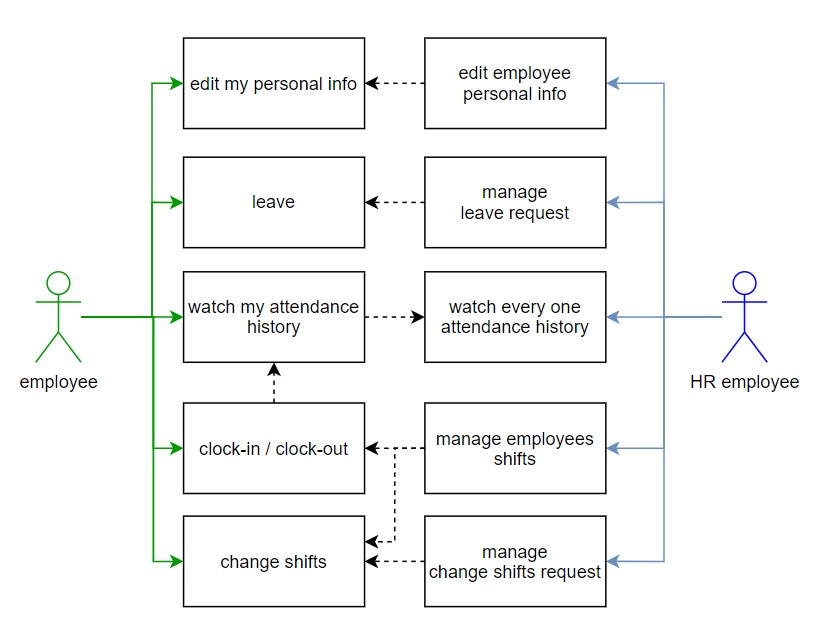
\includegraphics[width=10cm,keepaspectratio]{./images/penhwang_er_diagram_2.jpg}
\end{center}
\caption[แสดง use case diagram]{แสดง use case diagram ซึ่งแสดงให้เห็นกลุ่มผู้ใช้งานทั้ง 2 กลุ่มประกอบด้วย พนักงานทั่วไป (employee) และ พนักงาน hr (human resources employee)}
\end{figure}

\begin{figure}
\begin{center}
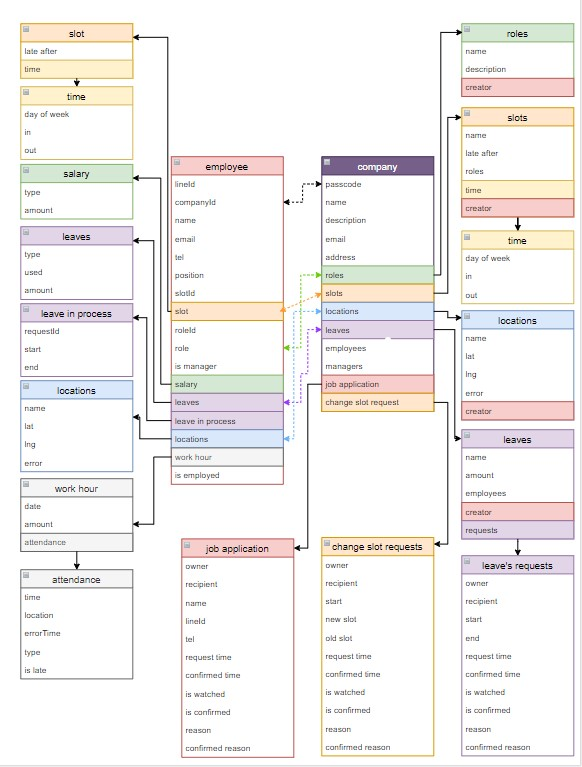
\includegraphics[width=14cm,keepaspectratio]{./images/penhwang_db_schema.jpg}
\end{center}
\caption[แสดง E-R diagram]{แสดง E-R diagram (Entity-Relationship diagram) ซึ่งแสดงรายละเอียดของข้อมูลของแต่ละ entity ประกอบด้วย พนักงาน และ บริษัท}
\end{figure}

\begin{figure}
\begin{center}
\includegraphics[width=14cm,keepaspectratio]{./images/structure.jpg}
\end{center}
\caption[แสดงโครงสร้างของระบบ]{
  แสดงโครงสร้างของระบบ ซึ่งแบ่งเป็น 2 ส่วนใหญ่ ๆ คือ 
  front-end ประกอบด้วย LINE application (LINE bot) และ Nuxt.js 
  และ back-end (Google firebase) ซึ่งประกอบด้วย firebase cloud functions และ firebase firestore 
  โดย มี Google dialogflow ขั้นกลางระหว่าง LINE application และ firebase เพื่อทำหน้าที่แปลความหมายข้อความ
}
\end{figure}
\chapter{\ifproject%
\ifcpe การทดลองและผลลัพธ์\else Experimentation and Results\fi
\else%
\ifcpe การทดลองและผลลัพธ์\else System Evaluation\fi
\fi}
\quad ในบทนี้จะกล่าวถึงการนำ prototype ไปทดสอบกับกลุ่มผู้ใช้งาน (potential user) โดยจะเป็นการให้โจทย์กับผู้ทดสอบแล้วปล่อยให้ใช้งาน prototype โดยใช้ความรู้สึก และ ความเคยชินของผู้ทดสอบเอง 
เพื่อที่จะวัดว่าระบบของเรามีความสอดคล้องกับ ux ของผู้ทดสอบเพียงใดและต้องปรับปรุงตรงไหนบ้าง โดยโจทย์ที่ให้กับผู้ทดสอบมีดังนี้ \ref{fig:eval_test}

\section{สร้างบริษัทของคุณ} 
ในขั้นตอนนี้ผู้ทดสอบจะต้องทำการกดปุ่มสร้างบริษัทใหม่ในหน้าแรก ดังรูป \ref{fig:index} จากนั้นระบบก็จะแสดงวิธีการสร้างบริษัทใหม่ดังรูป \ref{fig:create_company}
และ หากทำตามขั้นตอนที่เขี่ยนไว้ในวิธีการ คือ 1. เพิ่มเพื่อนกับ PenHwang โดยใช้การสแกน qr code หรือ ค้นหาชื่อ 2. พิมพ์คำว่า "สร้างบริษัทใหม่" 3. นำรหัสที่ตอบกลับมาไปใส่ในช่องที่กำหนด
ก็จะไปถึงหน้าตั้งค่าบริษัท ดังรูป \ref{fig:setting} จากนั้นทำการกรอกข้อมูลเบื้องต้นของบริษัทประกอบด้วย ชื่อ คำบรรยาย email เบอร์โทรศัพท์ และ ที่อยู่ของบริษัท

เนื่องจากผู้พัฒนาคิดว่าคนที่สร้างบริษัทก็จะเป็นพนักงานคนนึง จึงได้สร้างพนักงานโดยใช้ LINE id ของคนที่สร้างบริษัท ขั้นตอนต่อไปจึงเป็นการกรอกข้อมูลส่วนตัวของผู้สร้างบริษัท 
โดยการไปที่หน้าผู้จัดการ ดังรูป \ref{fig:manager} จากนั้นก็กรอกข้อมูลส่วนตัวของตนเองลงไปเป็นอันเสร็จขั้นตอนการสร้างบริษัท

ในขั้นแรกผู้ทดสอบสามารถทำได้แบบไม่ติดขัดอะไรนั้นแสดงว่า ux ณ จุดนี้ดีอยู่แล้ว แต่ผู้ทดสอบทำได้ราบรื่นจนถึงขั้นตอนการตั้งค่าเท่านั้น การกรอกข้อมูลส่วนตัวของตนเองนั้นยังต้องมีการบอกให้ทำ
นั้นแสดงว่า ต้องเพิ่มการสอนการเพิ่มผู้สร้างบริษัทเข้าสู่บริษัทด้วย และ มีคำแนะนำจากผู้ทดสอบว่าปุ่มลบบริษัทเด่นนั้นจนเกินไป และ ตอนสร้างบริษัทไม่ควรมีปุ่มนี้อยู่

\section{เพิ่มพนักงานอีก 1 คนเข้าสู่บริษัท}
ในขั้นตอนนี้ผู้ทดสอบต้องให้พนักงานอีกคนเพิ่มเพื่อนกับ PenHwang จากนั้นพิมพ์คำว่า "ฉันเป็นพนักงานใหม่" จะมี button message ตอบกลับมา ดังรูป \ref{fig:message_start_form}
เมื่อคลิ๊กเข้าไปแล้วจะเป็นแบบฟอร์มการเริ่มต้นเป็นพนังงานให้กรอกข้อมูลซี้งประกอบด้วย รหัสสำหรับบริษัท (passcode) ซึ่งได้จากหน้าตั้งค่าบริษัท \ref{fig:setting} และ ข้อมูลส่วนตัว เช่น ชื่อ เบอร์ติดต่อ email และ LINE id ดังรูป \ref{fig:line_start_form} 
จากนั้นหากกดส่ง 
ก็จะเป็นการส่งคำขอเข้าร่วมบริษัทไปที่บริษัทนั้น จากนั้นพนักงานฝ่ายบุคคลก็จะเป็นคนรับคำขอที่หน้า dashboard ดังรูป \ref{fig:dashboard} หรือ หน้าพนักงาน ดังรูป \ref{fig:new_employee}

ในขั้นตอนนี้ทางผู้พัฒนาไม่ได้ใส่จุดที่สอนวิธีการเพิ่มพนักงานเพราะผู้พัฒนาคิดว่าขั้นตอนการเพิ่มพนักงานอีก เหมือนกับการเพิ่มผู้สร้างบริษัททุกประการ แต่เมื่อทำการทดสอบแล้ว 
พบว่าผู้ทำการทดสอบไม่รู้ว่าต้องเพิ่มพนักงานอย่างไรทำให้ต้องบอกเป็นขั้นตอนเพื่อให้ไปถึงขั้นต่อไปได้

\section{สร้างตารางงานให้พนักงานคนนั้น}
ในขั้นตอนนี้ผู้ทดสอบต้องเข้าไปที่หน้า ตารางงานหรือกะ \ref{fig:slot} จะพบว่ามีกะที่สร้างไว้อยู่แล้วชื่อ default slot ซึ่งเป็นกะที่เริ่มงาน 9.30 น. ออกงาน 17.30 น. ทุกวันยกเว้นวันอาทิตย์ที่ไม่ทำงาน 
ผู้พัฒนาทำการใส่เอาไว้เพื่อเป็นตัวอย่างการจัดตารางงานให้พนักงาน หรือ หากบริษัทใดมีการทำงานที่ใกล้เคียงกันก็สามารถเปลี่ยนการตั้งค่าเล็กน้อยแล้วใช้งานตารางนี้ได้ แต่ในขั้นตอนี้ผู้ทดสอบจะต้องไปที่หน้า 
สร้างตารางใหม่ จากนั้นก็จะมีตารางให้เริ่มกรอกข้อมูลซึ่งประกอบด้วย ชื่อตาราง สายหลังจากผ่านไป เวลาเข้า-ออกงานของแต่ละวัน และ พนักงานที่จะให้ใช้ตารางนี้ ดังรูป \ref{fig:new_slot} 
จากนั้นมื่อเพิ่มพนักงานเข้าสู่กะแล้วก็จะมีข้อความส่งไปที่พนักงานคนนั้นด้วย ดังรูป \ref{fig:added_slot}

ในขั้นตอนนี้ผู้ทดสอบมีความสับสนเล็กน้อยกับข้อความในหน้าสร้างตารางใหม่ คือ คำว่า "สายหลังจาก" ซึ่งความหมายของมันคือสายหลังจากผ่านไปกี่นาที แต่ผู้ทดสอบสับสนว่าเป็นสายหลังจากเวลาเท่าใด

\section{ให้พนักงานดูตารางเวลาทำงานของตนเอง}
ในขั้นตอนนี้ผู้ทดสอบต้องทำการกด rich menu ปุ่มดูตารางงานของฉันใน LINE ดังรูป \ref{fig:rich_menu} จากนั้นจะได้รับข้อความตอบกลับในรูแบบ flex message ที่บอกเวลาที่ต้องเข้า-ออกงานในแต่ละวัน ดังรูป \ref{fig:message_slot}

\section{สร้างจุดลงเวลา}
ในขั้นตอนนี้ผู้ทดสอบต้องไปที่หน้า จุดลงเวลา \ref{fig:location} และกดที่ปุ่มสร้างจุดลงเวลาใหม่ \ref{fig:new_location} จากนั้นก็กรอกข้อมูลซึ่งประกอบด้วย ชื่อจุดลงเวลา ระยะที่สามารถห่างได้ 
ผู้พัฒนาได้จำกัดระยะนี้ไว้น้อยสุดที่ 50 เมตรเพื่อป้องกัน ความผิดพลาดจากการเช็คตำแหน่งที่อยู่ จุดลงเวลาโดยใช้ Google map API มาแสดงและเก็บค่า และ พนักงานที่จะใช้จุดลงเวลานี้ 
จากนั้นมื่อเพิ่มพนักงานเข้าสู่กะแล้วก็จะมีข้อความส่งไปที่พนักงานคนนั้นด้วย \ref{fig:added_location}

\section{เช็คชื่อเข้า-ออกงาน}
ในขั้นตอนนี้ผู้ทดสอบต้องทำการกด rich menu ปุ่มขอลงเวลาใน LINE ดังรูป \ref{fig:rich_menu} จากนั้นจะได้รับข้อความตอบกลับในรูแบบ button message โดยหากไม่ได้เข้างานอยู่
จะเป็นข้อความเพื่อเข้างาน แต่ หากเข้างานอยู่แล้วข้อความที่ส่งมาก็จะเปลี่ยนเป็นข้อความเพื่อออกงาน ดังรูป \ref{fig:clock_in} และ \ref{fig:clock_out} เมื่อกด button message เข้าไปจะเป็น 
web applicaion ที่แสดงว่าสามารถเข้า หรือออกงานตรงนี้ได้หรือไม่ หาไม่ได้จะมีข้อความแสดงผลดังรูป \ref{fig:cant_clock} 
แต่หากสามารถเข้างานได้จะแสดงปุ่มเพื่อเข้า หรือออกงาน ดังรูป \ref{fig:clock} 
จากนั้นหากต้องการดูประวัตการเข้าออกงานของพนักงานสามารถเข้าไปดูได้ที่หน้าพนักงาน/เลือกพนักงานคนนั้น/ประวัติการทำงาน ดังรูป \ref{fig:history} โดยจะแสดงวันเวลาที่เข้า-ออก ลา หรือ ขาดงาน
ละเมื่อคลิ๊กที่การเข้าหรือออกงาน ก็จะเป็นการแสดงสถานที่ที่พนักงานคนนั้นเข้าหรือออกงานได้ด้วย
หรือ สามารถดูสรุปประวัติการทำงานของพนักงานทุกคนได้ที่หน้าเงินเดือน 
ส่วนพนักงานเองก็สามารถดูประวัติการเข้าออกงานของตนเองได้เหมือนกันโดยคลิ๊ก rich menu ปุ่มตั้งค่า จากนั้นจะได้รับข้อความตอบกลับในรูแบบ carousel button message 
ดังรูป \ref{fig:message_setting}
จากนั้นเลือก ข้อมูลส่วนตัว จะเป็นการเข้าสู่เว็บแอปพลิเคชันที่แสดงข้อมูลของพนักงานประกอบด้วย ข้อมูลส่วนตัว ประวัติการทำงาน และ สิทธิการลา ดังรูป \ref{fig:line_personal_info}

\section{สร้างประเภทการลา}
ในขั้นตอนนี้ผู้ทดสอบต้องเข้าไปที่หน้า \ref{fig:leave} ประเภทการลาและกดปุ่มสร้างประเภทใหม่ \ref{fig:new_leave} 
จากนั้นก็กรอกข้อมูลซึ่งประกอบด้วย ชื่อประเภทการลา สิทธิ์การลา และพนักงานที่สามารถใช้การลานี้ได้
และเมื่อเพิ่มพนักงานให้สามารถใช้ประเภทการลานั้น ๆ ได้ก็จะส่งข้อความไปหาพนักงานด้วยดังรูป \ref{fig:added_leave}

โดยในขั้นตอนการขอดูตารางเวลาทำงานขอตนเอง เช็คชื่อเข้าออกงาน และสร้างประเภทการลา ผู้ทดสอบสามารถทำได้โดยไม่ติดขัดอะไรตั้งแต่ต้นจนจบ
\section{ส่งแบบฟอร์มการลา}
ในขั้นตอนนี้ผู้ทดสอบต้องทำการกด rich menu ปุ่มคำขอใน Line \ref{fig:rich_menu} จากนั้นจะได้รับข้อความตอบกลับในรูแบบ button message ดังรูป \ref{fig:message_leave}
เมื่อคลิ๊กเข้าไปจะเป็นแบบฟอร์มการขอลาให้กรอกข้อมูลประกอบด้วย ประเภทการลา วันที่จะเริ่มละ วันจบการลา และ เหตุผลที่จะลา ดังรูป \ref{fig:line_leave} เมื่อส่งแล้ว 
คำขอจะไปปรากฎที่หน้า dashboard พนักงานฝ่ายบุคคลสามารถกดยืนยันหรือปฎิเสธได้ที่นี่ เมื่อคำขอได้รับการจัดการแล้วพนักงานจะได้รับข้อความตอบกลับและ สามารถดูประวัติย้อนหลังได้ที่หน้า 
ข้อมูลส่วนตัว/สิทธิการลา ดังรูป \ref{fig:line_leave_history}

ในขั้นตอนนี้ผู้ทดสอบให้ความเห็นว่าการตอบกลับของ penhwang ช้าไป เพราะเมื่อส่งข้อความก็ขึ้นเลยว่าอ่านแล้วแต่ต้องรออีกประมาณ 5-10 วินาทีถึงจะมีข้อความตอบกลับมา
\section{ขอเข้าสู่ระบบ สำหรับพนักงานฝ่ายบุคคลเท่านั้น}
ในขั้นตอนนี้จะมีสอนในหน้าแรก โดยขั้นตอนคือกดปุ่มเข้าสู่ระบบ แล้วกด rich menu ใน LINE ปุ่มตั้งค่า จากนั้นเลือก เข้าสู่ระบบ \ref{fig:login}
หากเป็นพนังงานฝ่ายบุคคล (มีรายชื่อในผู้จัดการของบริษัท) จะมีรหัสตอบกลับมา ดังรูป \ref{fig:message_login}
จากนั้นนำรหัสมาใส่ในเว็บ ฯ ก็จะสามารถเข้าสู่ระบบได้

\begin{figure}
  \begin{center}
    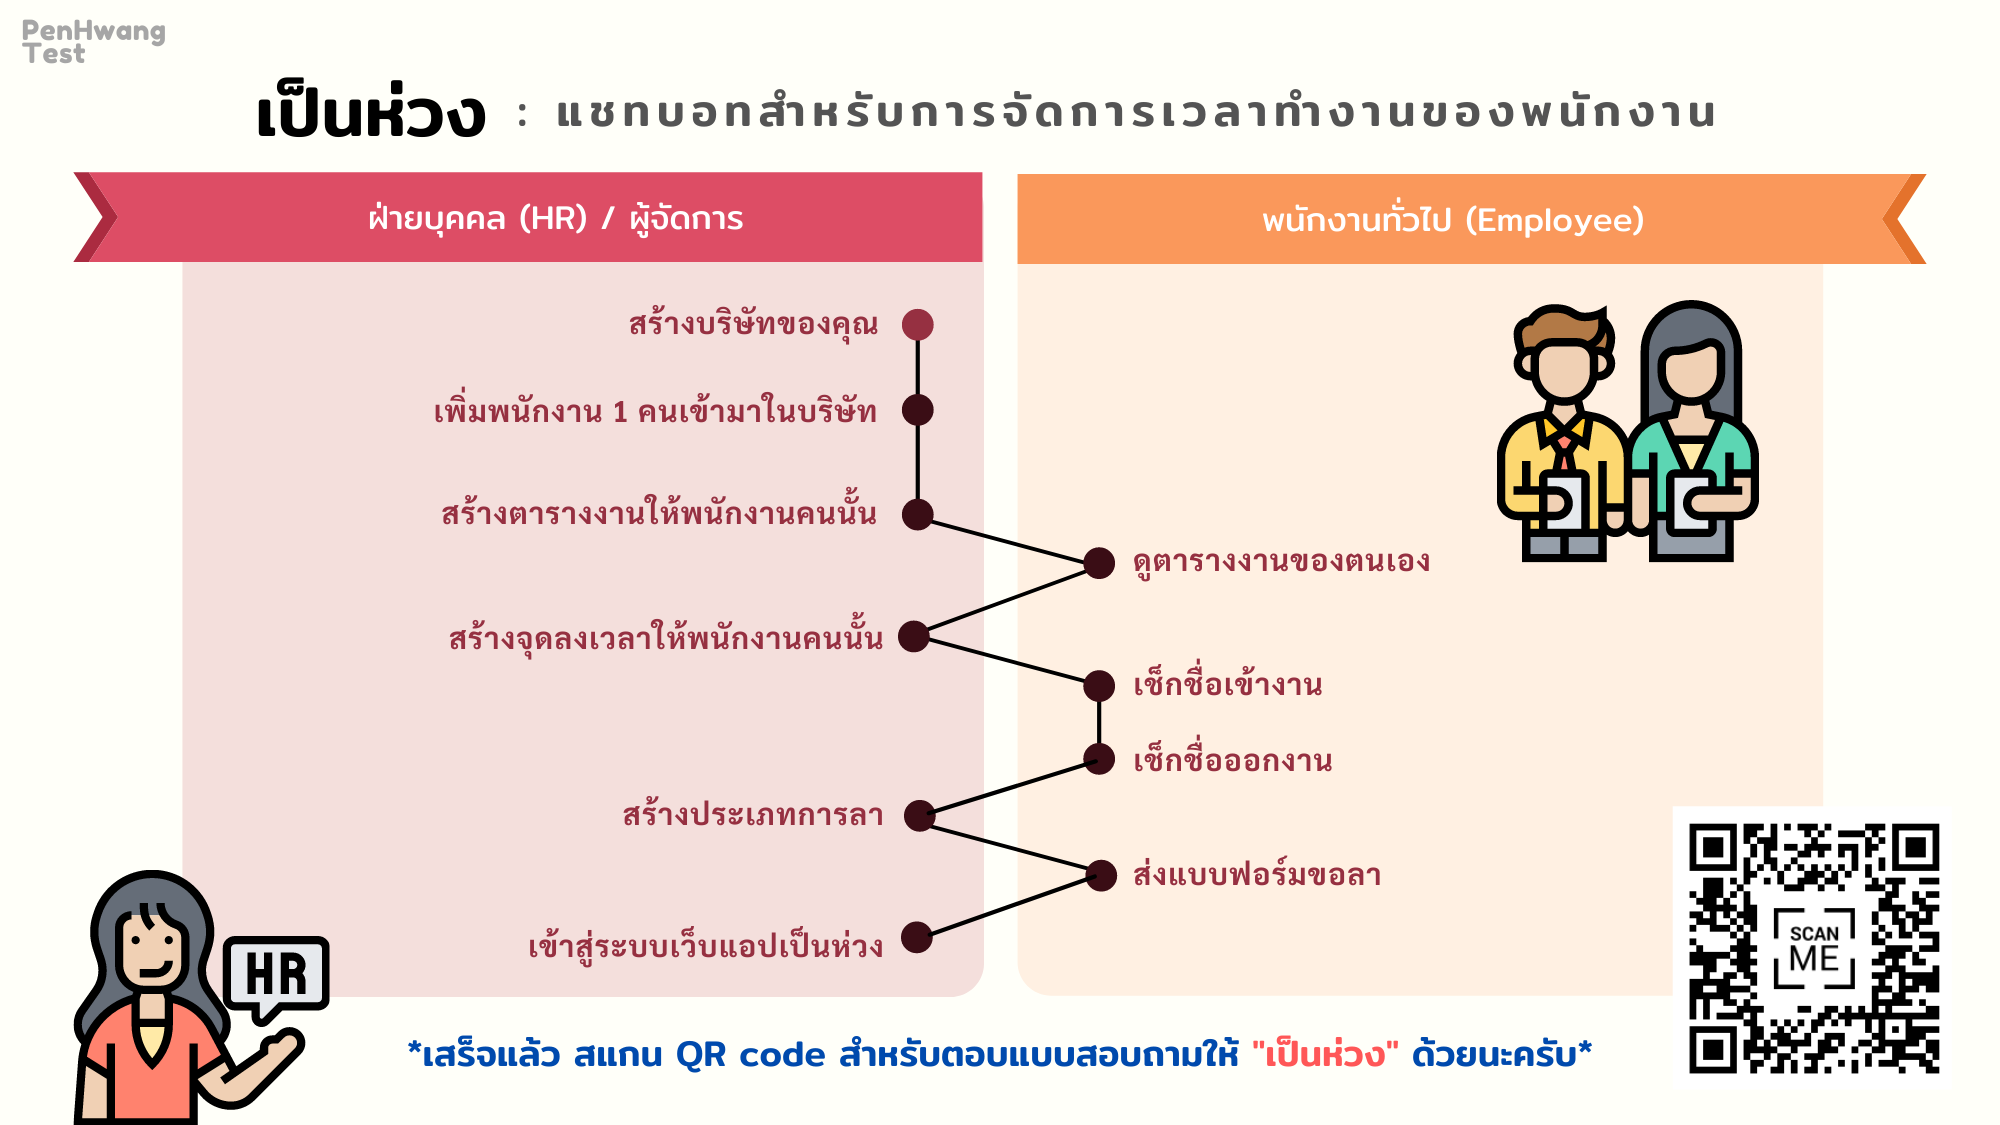
\includegraphics[width=14cm,keepaspectratio]{./images/test_flow.png}
  \end{center}
  \caption[รูปแสดงโจทย์ที่ส่งให้ผู้ทดสอบลองทำตาม]{รูปแสดงโจทย์ที่ส่งให้ผู้ทดสอบลองทำตาม} 
  \label{fig:eval_test}
\end{figure}

\begin{figure}
  \begin{center}
    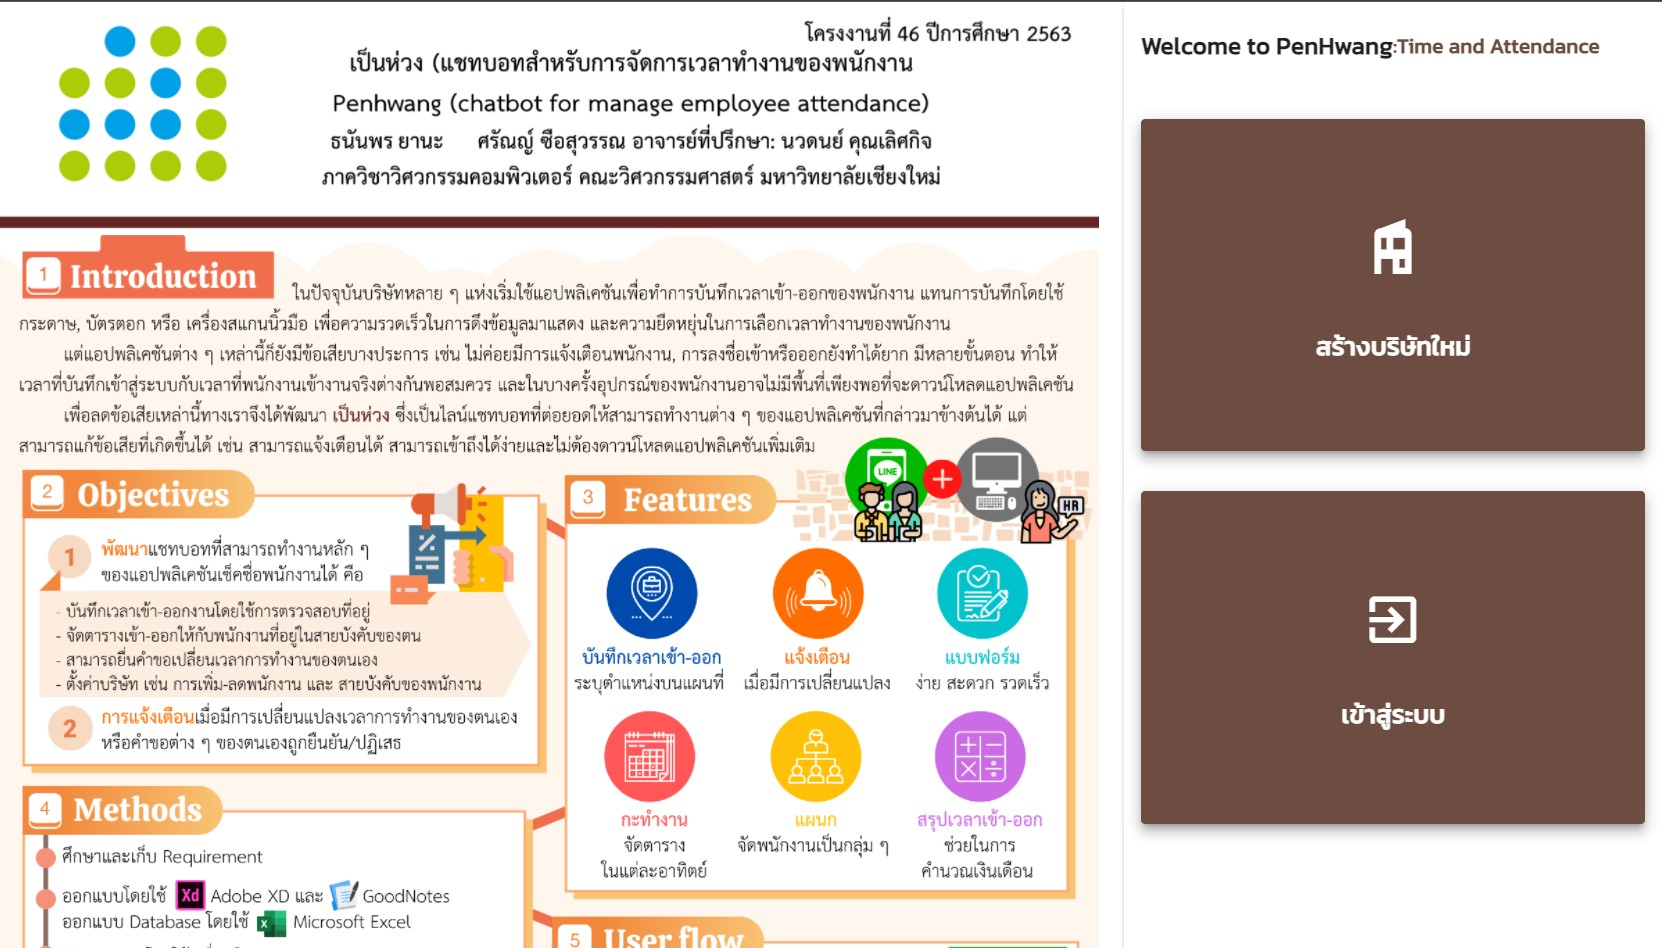
\includegraphics[width=14cm,keepaspectratio]{./images/index.jpg}
  \end{center}
  \caption[รูปแสดงหน้าแรกของเว็บแอปพลิเคชันเป็นห่วง]{รูปแสดงหน้าแรกของเว็บแอปพลิเคชันเป็นห่วง} 
  \label{fig:index}
\end{figure}

\begin{figure}
  \begin{center}
    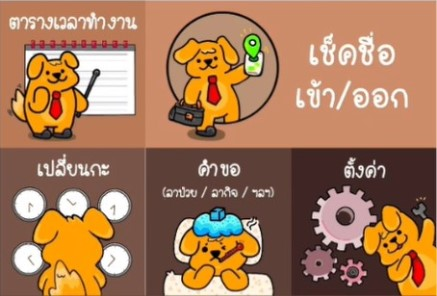
\includegraphics[width=7cm,keepaspectratio]{./images/rich_menu.jpg}
  \end{center}
  \caption[รูปแสดง rich menu ใน LINE]{รูปแสดง rich menu ใน LINE} 
  \label{fig:rich_menu}
\end{figure} 

\begin{figure}
  \begin{center}
    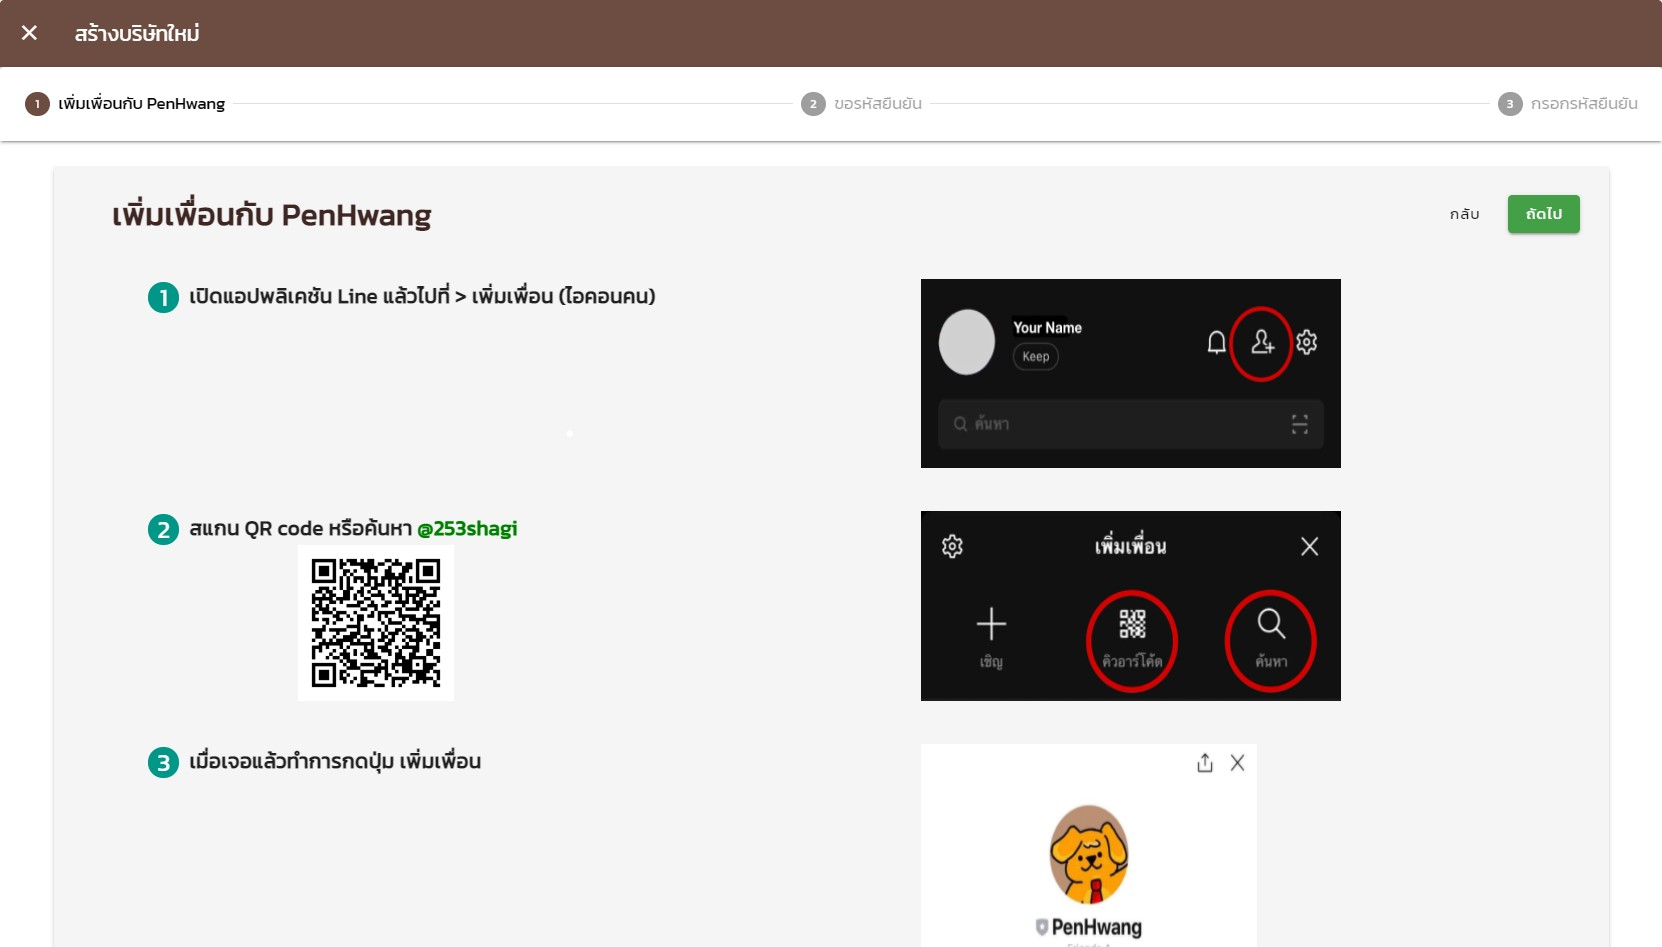
\includegraphics[width=14cm,keepaspectratio]{./images/create_company.jpg}
  \end{center}
  \caption[รูปแสดงวิธีการสร้างบริษัทใหม่]{รูปแสดงวิธีการสร้างบริษัทใหม่} 
  \label{fig:create_company}
\end{figure}

\begin{figure}
  \begin{center}
    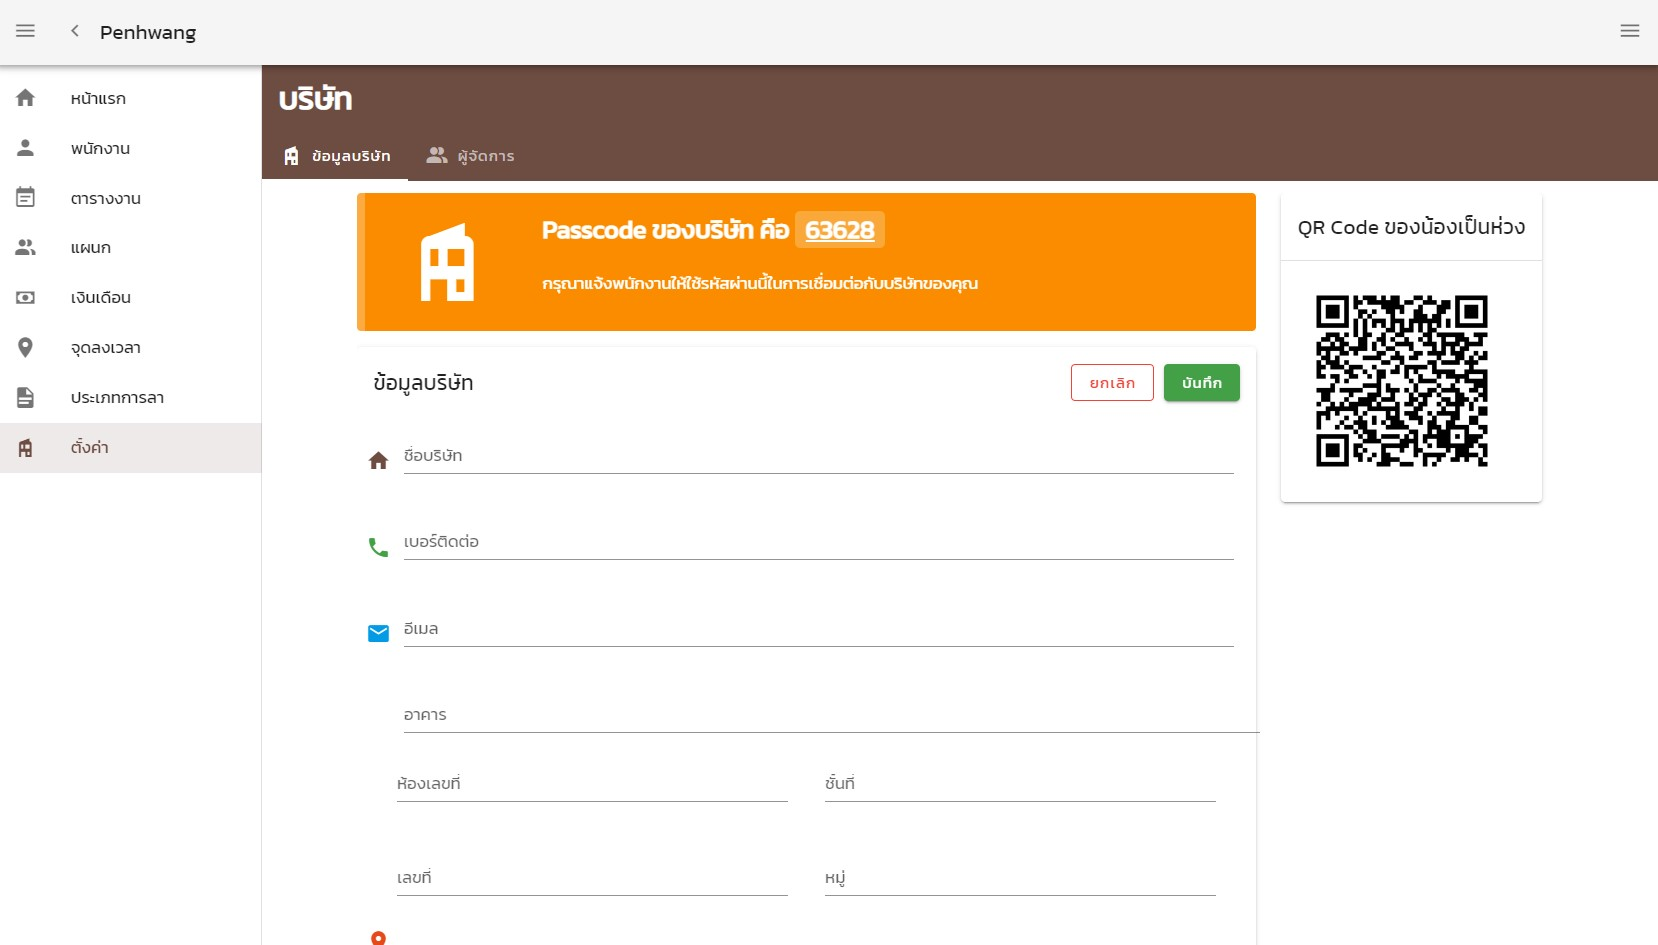
\includegraphics[width=14cm,keepaspectratio]{./images/setting.jpg}
  \end{center}
  \caption[รูปแสดงหน้าตั้งค่าบริษัท]{รูปแสดงหน้าตั้งค่าบริษัท} 
  \label{fig:setting}
\end{figure}

\begin{figure}
  \begin{center}
    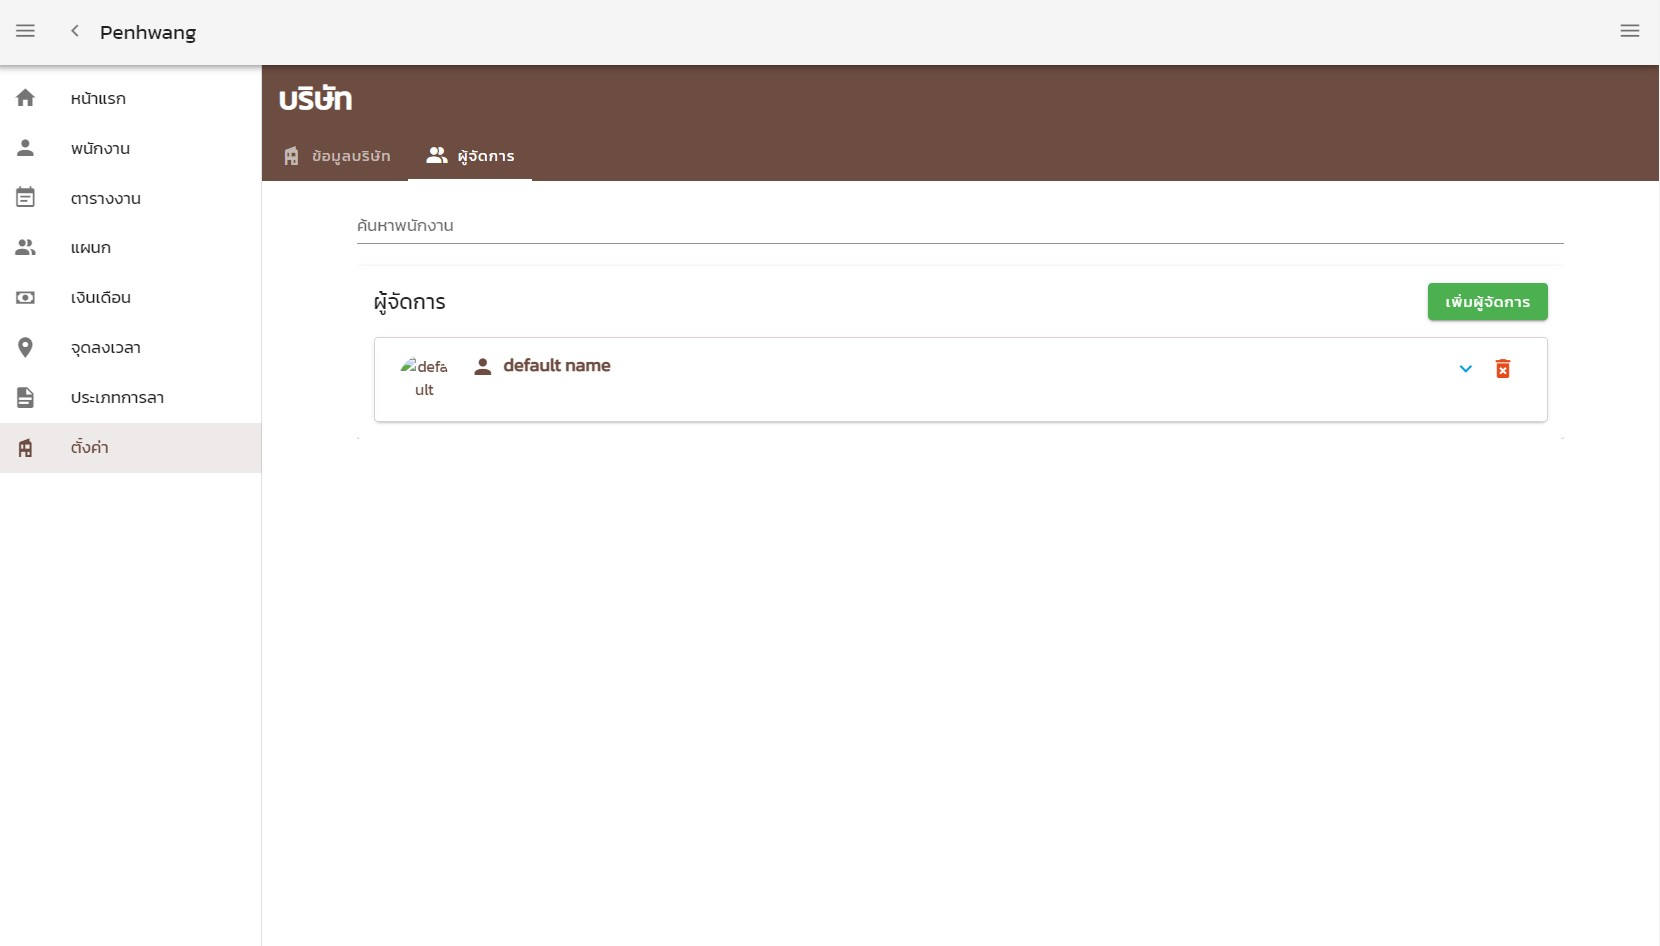
\includegraphics[width=14cm,keepaspectratio]{./images/manager.jpg}
  \end{center}
  \caption[รูปแสดงหน้าจัดการผู้จัดการ/พนักงานฝ่ายบุคคลของบริษัท]{รูปแสดงหน้าจัดการผู้จัดการ/พนักงานฝ่ายบุคคลของบริษัท} 
  \label{fig:manager}
\end{figure}

\begin{figure}
  \begin{center}
    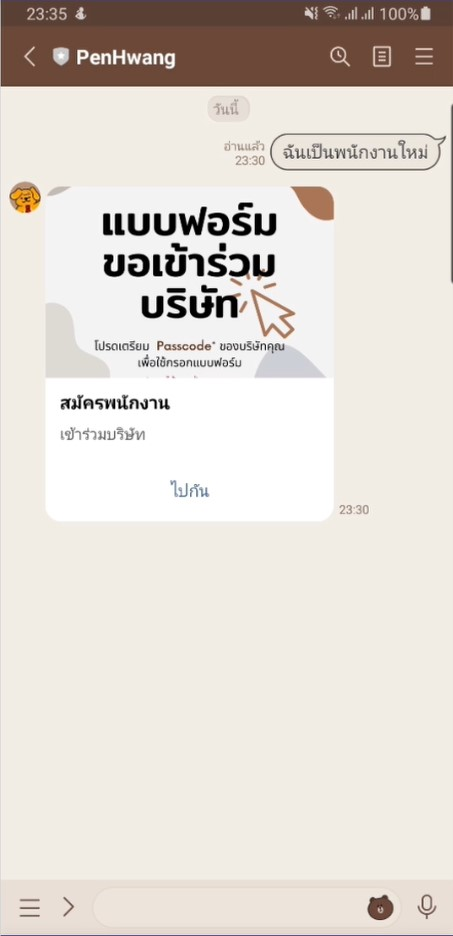
\includegraphics[width=4cm,keepaspectratio]{./images/message_start_form.jpg}
  \end{center}
  \caption[รูปแสดงข้อความตอบกลับเมื่อขอเป็นพนักงานใหม่]{รูปแสดงข้อความตอบกลับเมื่อขอเป็นพนักงานใหม่} 
  \label{fig:message_start_form}
\end{figure}

\begin{figure}
  \begin{center}
    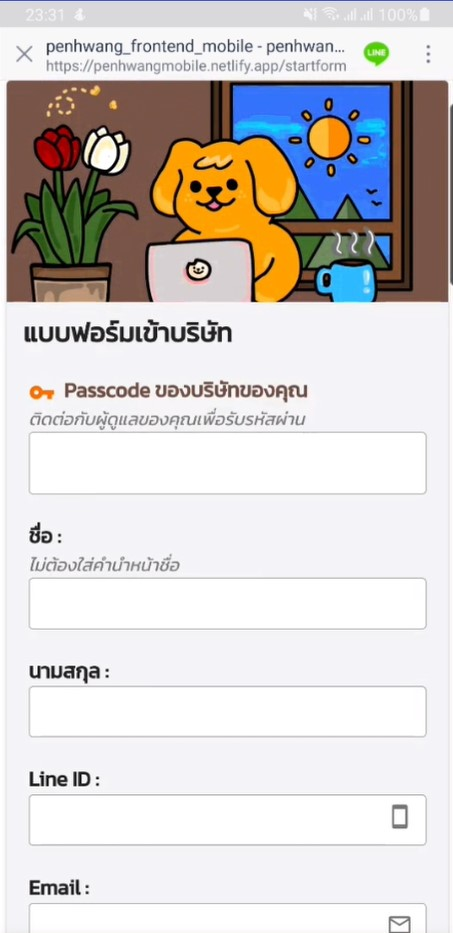
\includegraphics[width=4cm,keepaspectratio]{./images/line_start_form.jpg}
  \end{center}
  \caption[รูปแสดงแบบฟอร์มเข้าร่วมบริษัท]{รูปแสดงแบบฟอร์มเข้าร่วมบริษัท} 
  \label{fig:line_start_form}
\end{figure}

\begin{figure}
  \begin{center}
    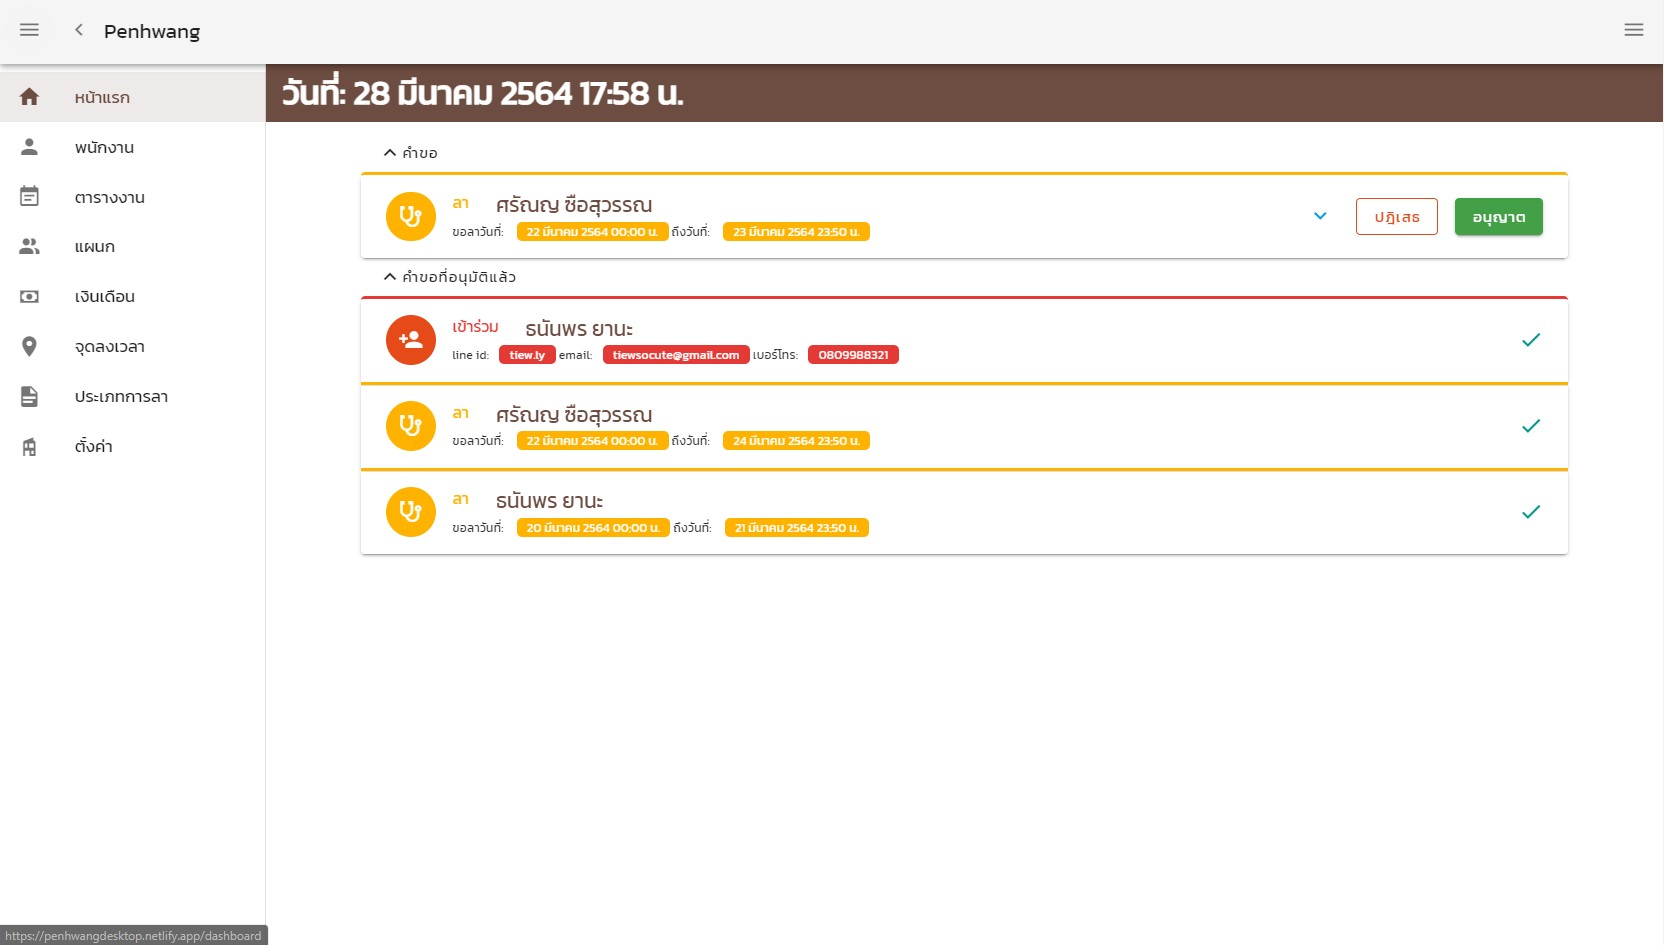
\includegraphics[width=14cm,keepaspectratio]{./images/dashboard.jpg}
  \end{center}
  \caption[รูปแสดงหน้าสรุปคำขอจากพนักงาน]{รูปแสดงหน้าสรุปคำขอจากพนักงาน} 
  \label{fig:dashboard}
\end{figure}

\begin{figure}
  \begin{center}
    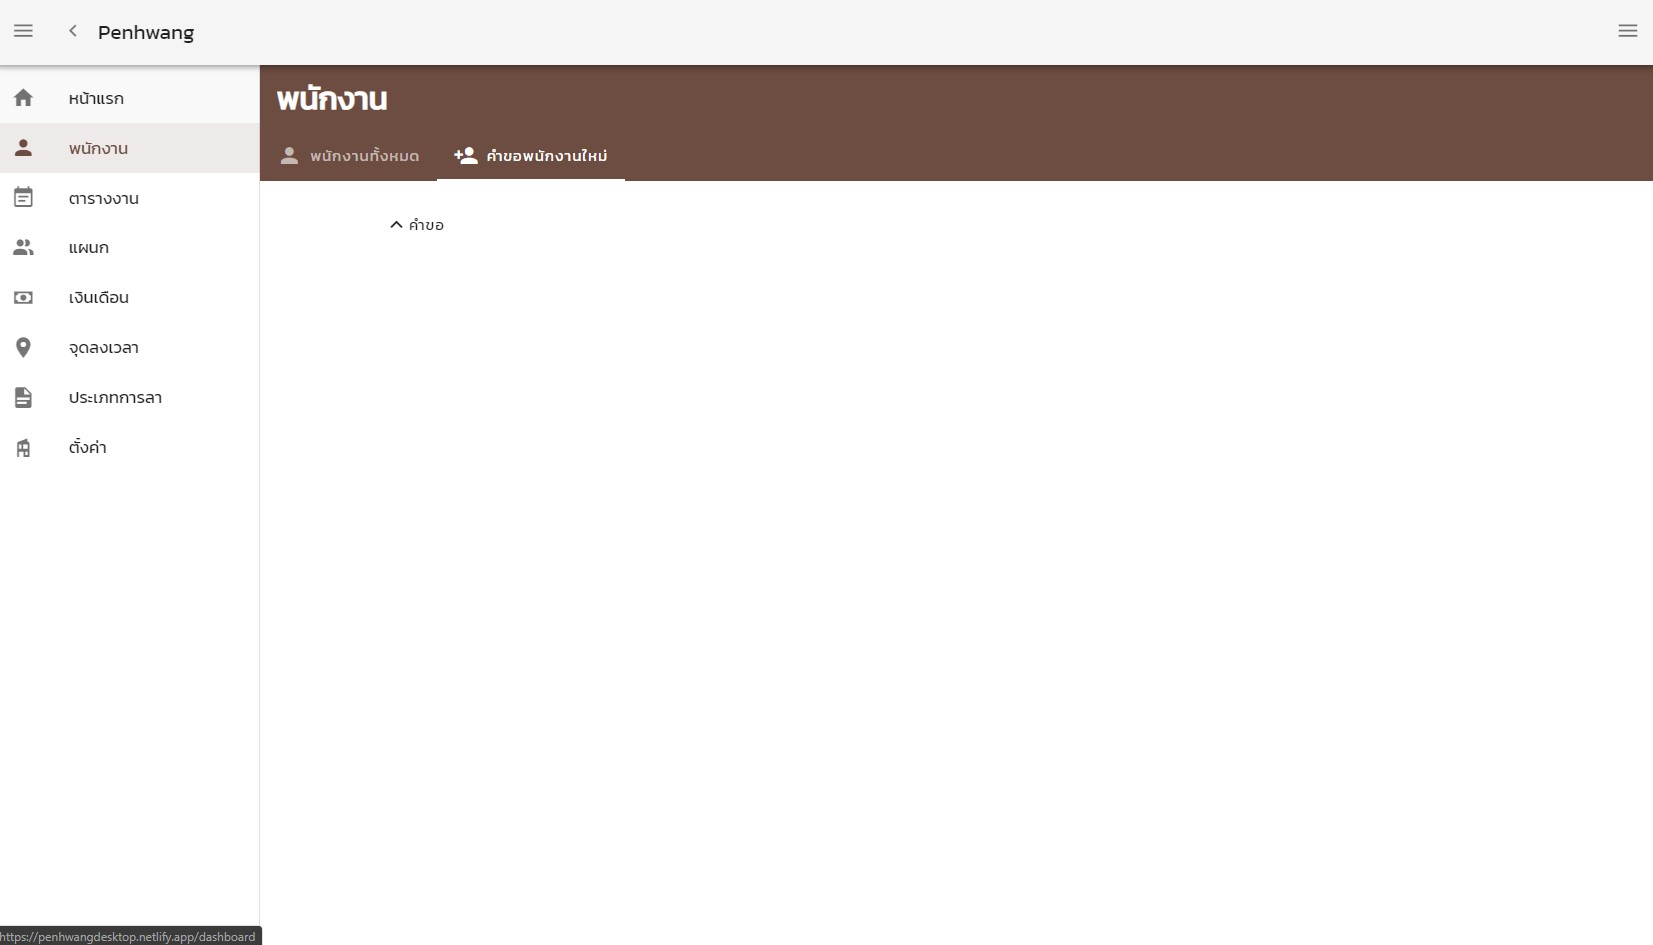
\includegraphics[width=14cm,keepaspectratio]{./images/new_employee.jpg}
  \end{center}
  \caption[รูปแสดงหน้าพนักงานใหม่]{รูปแสดงหน้าพนักงานใหม่} 
  \label{fig:new_employee}
\end{figure}

\begin{figure}
  \begin{center}
    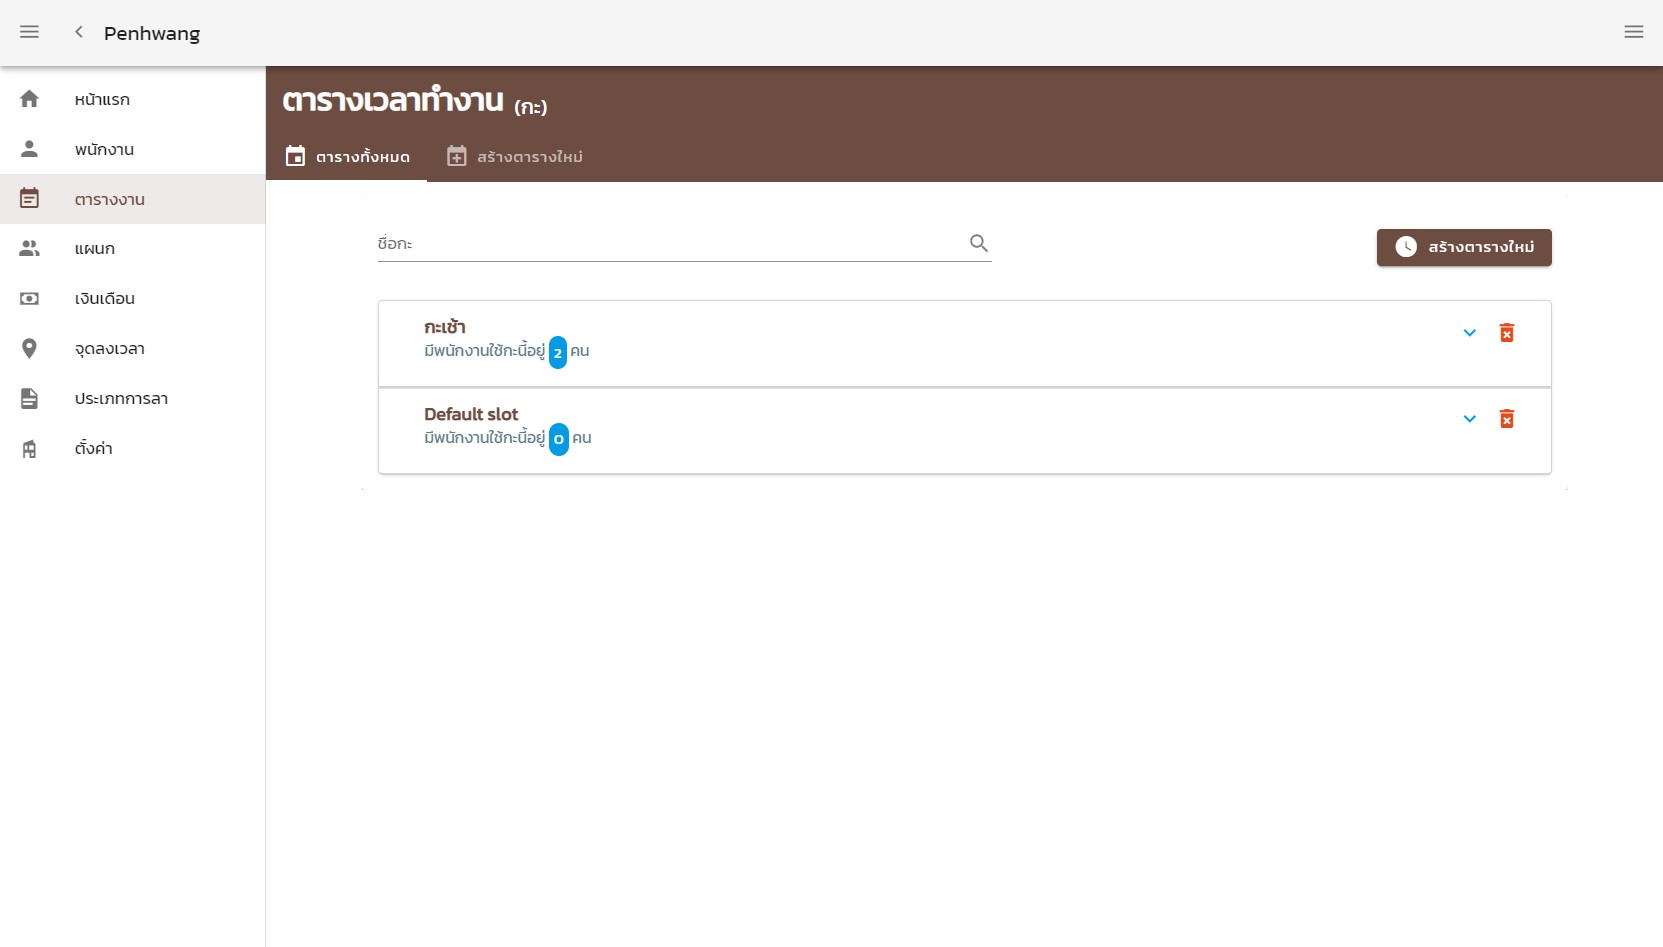
\includegraphics[width=14cm,keepaspectratio]{./images/slot.jpg}
  \end{center}
  \caption[รูปแสดงหน้ารวมของตารางเวลาทำงาน/กะ]{รูปแสดงหน้ารวมของตารางเวลาทำงาน/กะ} 
  \label{fig:slot}
\end{figure}
 
\begin{figure}
  \begin{center}
    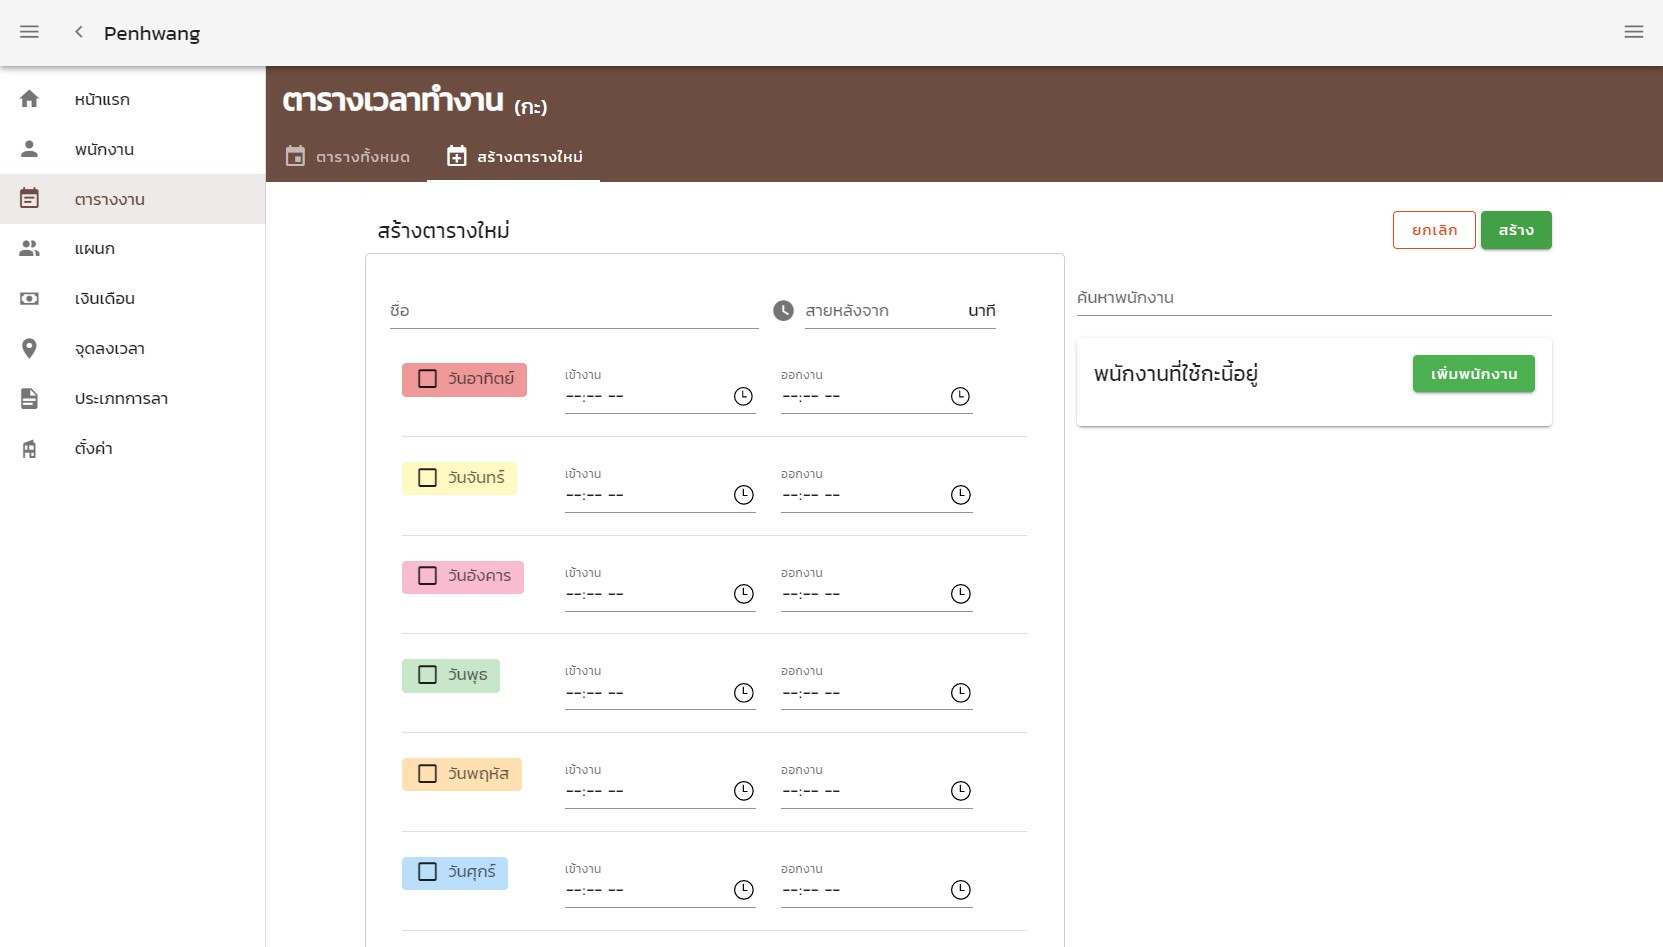
\includegraphics[width=14cm,keepaspectratio]{./images/new_slot.jpg}
  \end{center}
  \caption[รูปแสดงหน้าสร้างกะใหม่]{รูปแสดงหน้าสร้างกะใหม่} 
  \label{fig:new_slot}
\end{figure}
 
\begin{figure}
  \begin{center}
    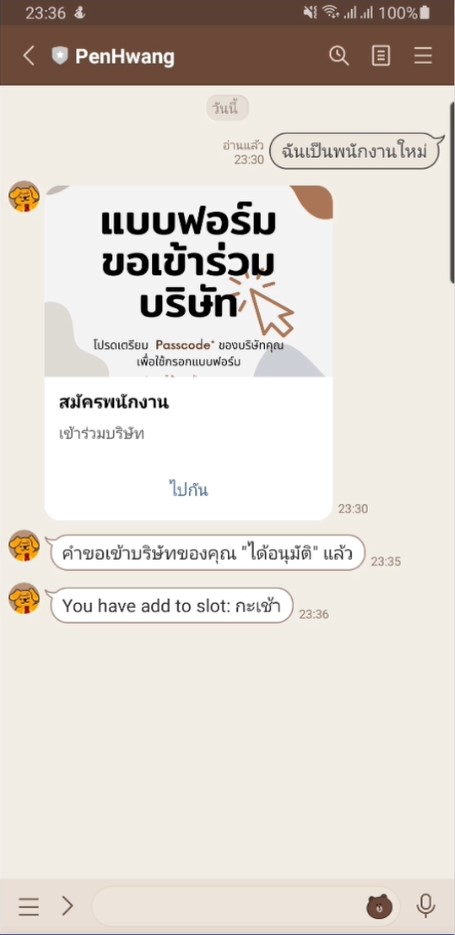
\includegraphics[width=4cm,keepaspectratio]{./images/added_slot.jpg}
  \end{center}
  \caption[รูปแสดงข้อความเมื่อกะมีการเปลี่ยนแปลง]{รูปแสดงข้อความเมื่อกะมีการเปลี่ยนแปลง} 
  \label{fig:added_slot}
\end{figure}

\begin{figure}
  \begin{center}
    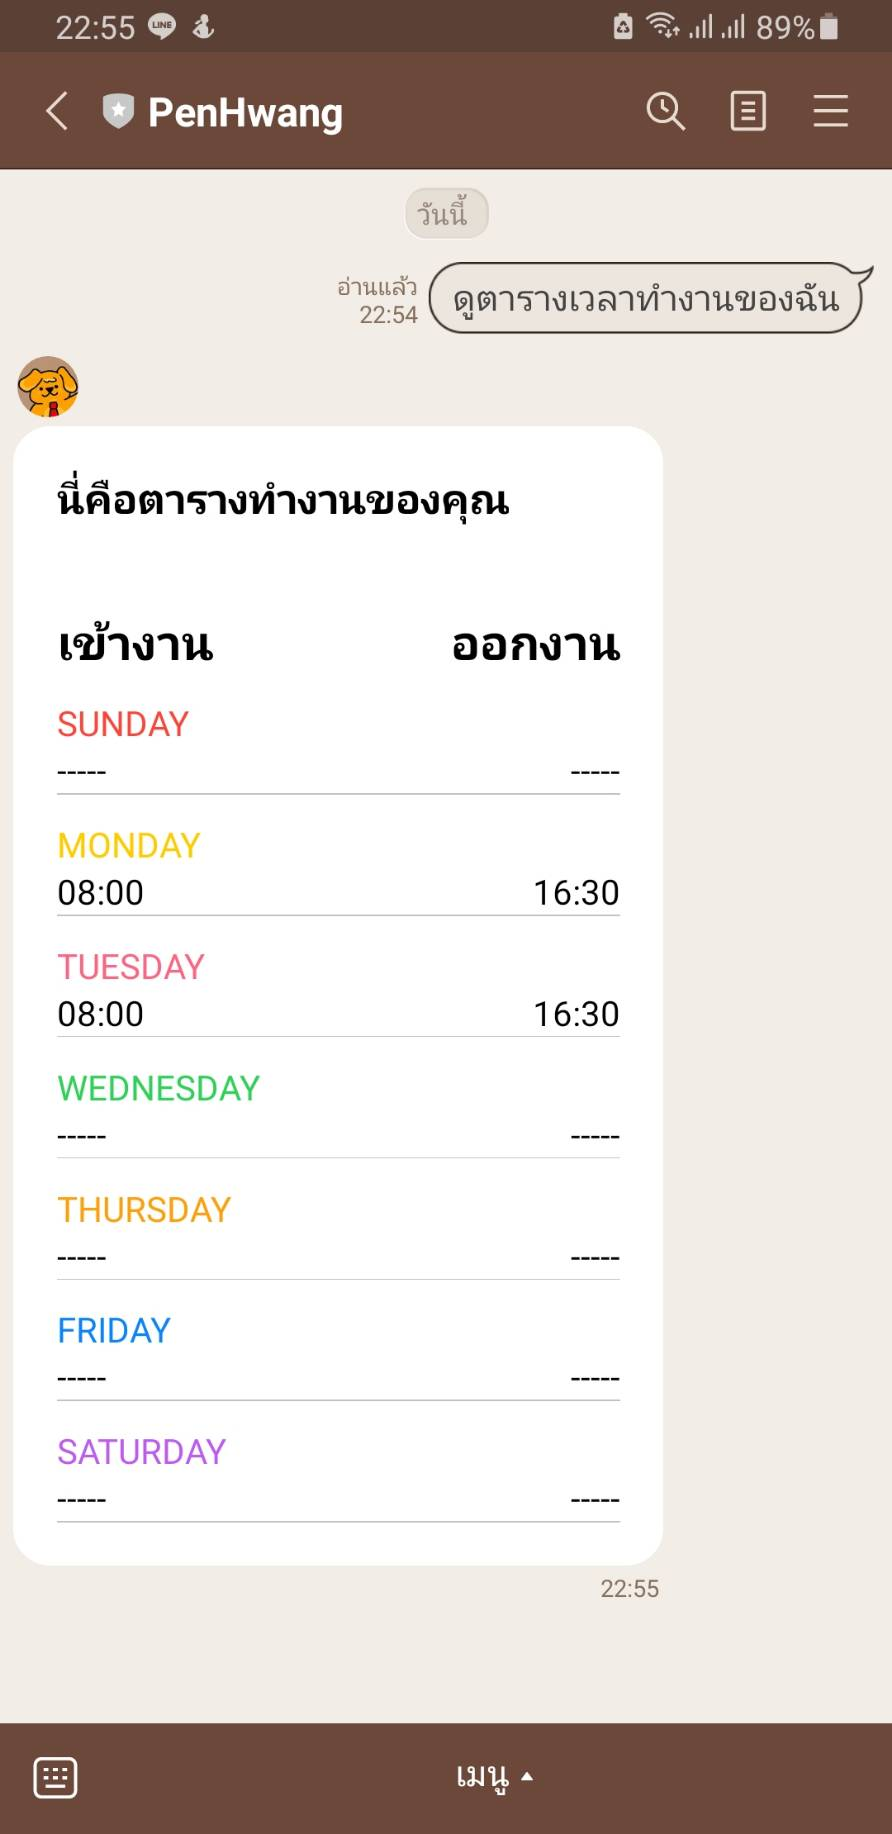
\includegraphics[width=4cm,keepaspectratio]{./images/message_slot.jpg}
  \end{center}
  \caption[รูปแสดงข้อความบอกตารางเวลาทำงานของพนักงาน]{รูปแสดงข้อความบอกตารางเวลาทำงานของพนักงาน} 
  \label{fig:message_slot}
\end{figure}

\begin{figure}
  \begin{center}
    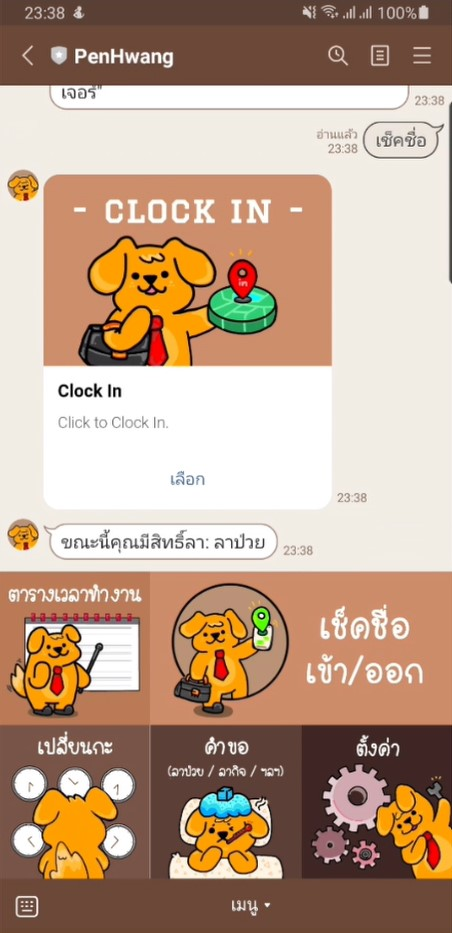
\includegraphics[width=4cm,keepaspectratio]{./images/added_leave.jpg}
  \end{center}
  \caption[รูปแสดงข้อความเมื่อมีการเพิ่ม/ยกเลิกประเภทการลาของพนักงาน]{รูปแสดงข้อความเมื่อมีการเพิ่ม/ยกเลิกประเภทการลาของพนักงาน} 
  \label{fig:added_leave}
\end{figure}

\begin{figure}
  \begin{center}
    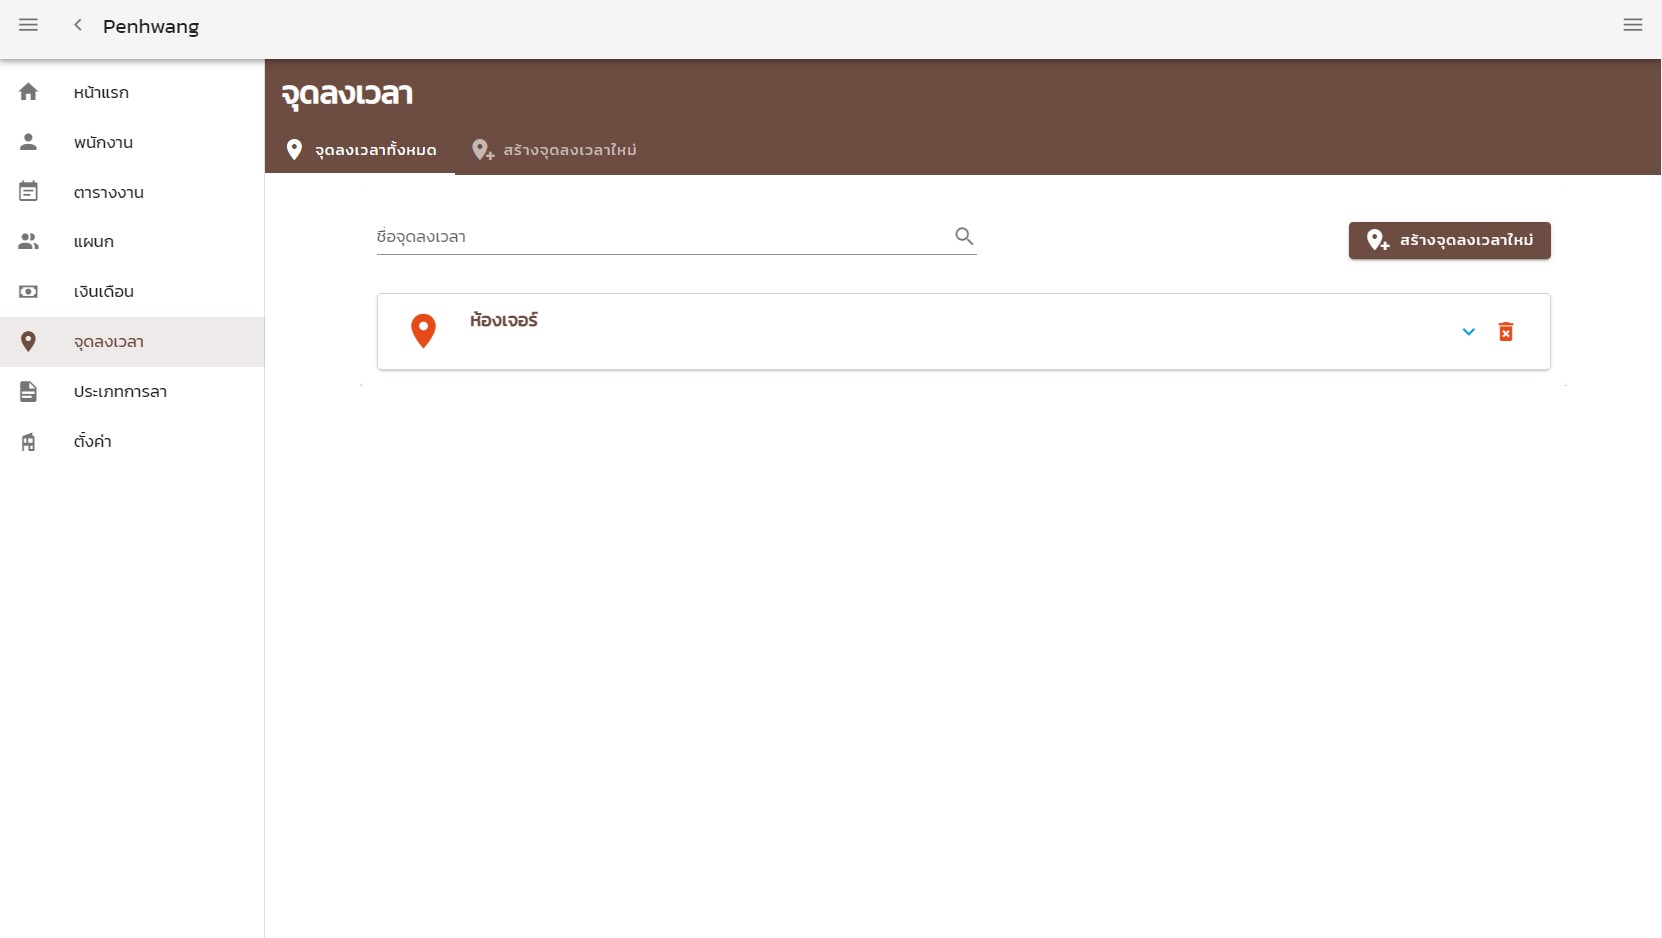
\includegraphics[width=14cm,keepaspectratio]{./images/location.jpg}
  \end{center}
  \caption[รูปแสดงหน้ารวมของจุดลงเวลา]{รูปแสดงหน้ารวมของจุดลงเวลา} 
  \label{fig:location}
\end{figure}
 
\begin{figure}
  \begin{center}
    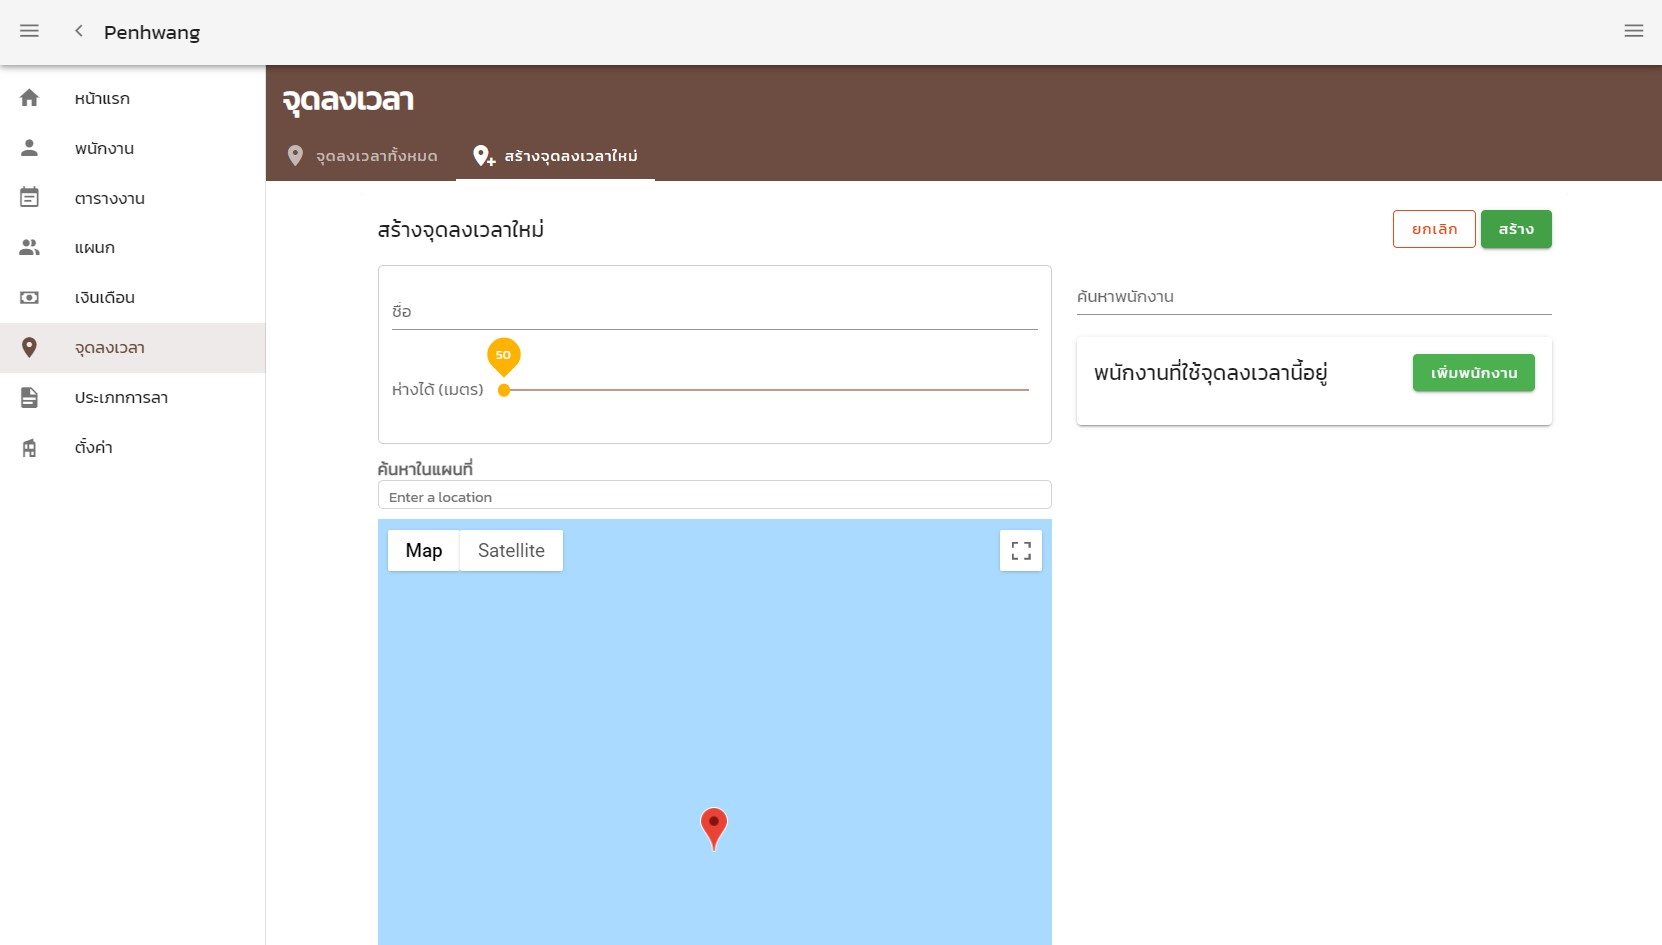
\includegraphics[width=14cm,keepaspectratio]{./images/new_location.jpg}
  \end{center}
  \caption[รูปแสดงหน้าสร้างจุดลงเวลาใหม่]{รูปแสดงหน้าสร้างจุดลงเวลาใหม่} 
  \label{fig:new_location}
\end{figure}
 
\begin{figure}
  \begin{center}
    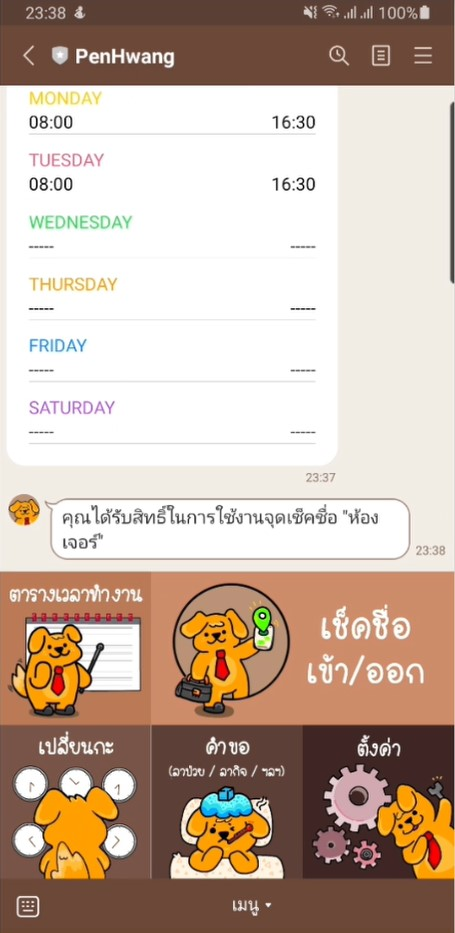
\includegraphics[width=4cm,keepaspectratio]{./images/added_location.jpg}
  \end{center}
  \caption[รูปแสดงข้อความเมื่อได้รับสิทธิ์ในการลงเวลาที่จุดลงเวลาใหม่]{รูปแสดงข้อความเมื่อได้รับสิทธิ์ในการลงเวลาที่จุดลงเวลาใหม่} 
  \label{fig:added_location}
\end{figure}

\begin{figure}
  \begin{center}
    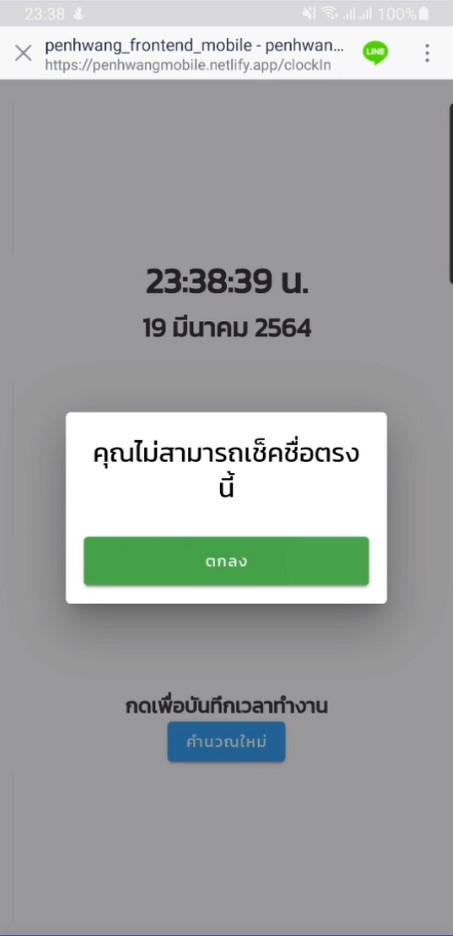
\includegraphics[width=4cm,keepaspectratio]{./images/cant_clock.jpg}
  \end{center}
  \caption[รูปแสดงข้อความเมื่อไม่สามารถลงเวลา ณ จุดนี้ได้]{รูปแสดงข้อความเมื่อไม่สามารถลงเวลา ณ จุดนี้ได้} 
  \label{fig:cant_clock}
\end{figure}
 
\begin{figure}
  \begin{center}
    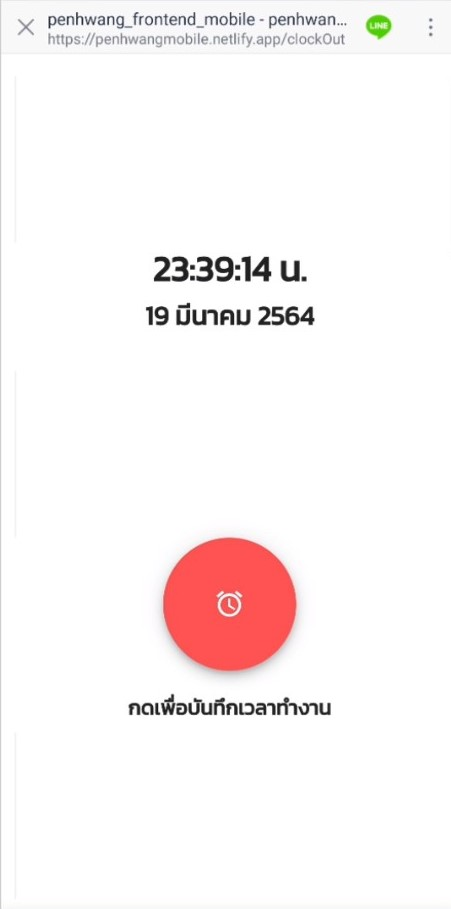
\includegraphics[width=4cm,keepaspectratio]{./images/clock.jpg}
  \end{center}
  \caption[รูปแสดงหน้าจอ เมื่อสามารถลงเวลา ณ จุดนี้ได้]{รูปแสดงหน้าจอ เมื่อสามารถลงเวลา ณ จุดนี้ได้} 
  \label{fig:clock}
\end{figure}

\begin{figure}
  \begin{center}
    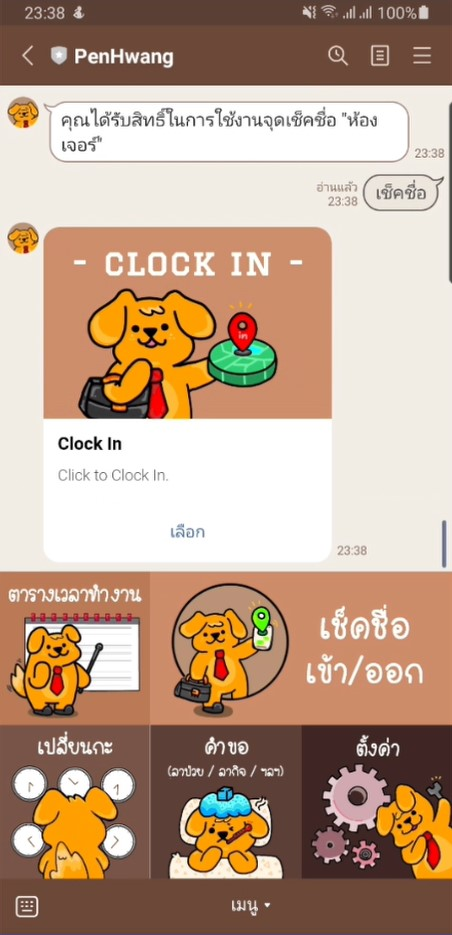
\includegraphics[width=4cm,keepaspectratio]{./images/clock_in.jpg}
  \end{center}
  \caption[รูปแสดงข้อความตอบกลับเมื่อขอเข้างาน]{รูปแสดงข้อความตอบกลับเมื่อขอเข้างาน} 
  \label{fig:clock_in}
\end{figure}
 
\begin{figure}
  \begin{center}
    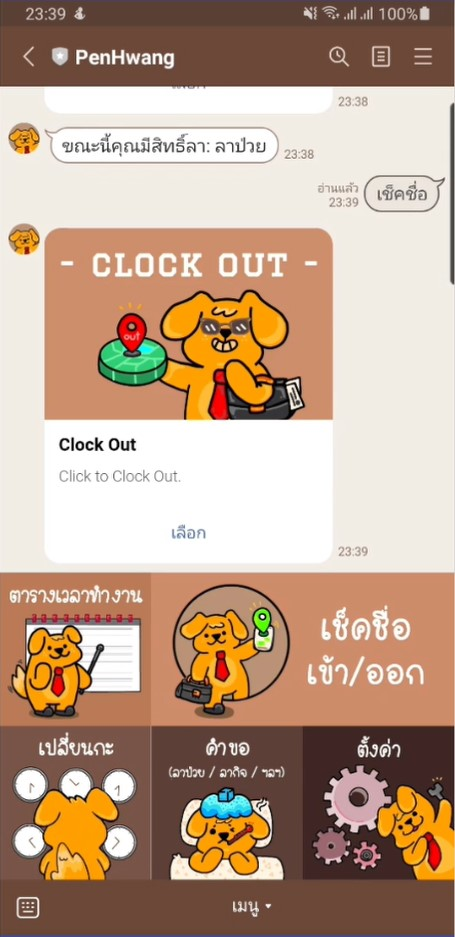
\includegraphics[width=4cm,keepaspectratio]{./images/clock_out.jpg}
  \end{center}
  \caption[รูปแสดงข้อความตอบกลับเมื่อขอออกงาน]{รูปแสดงข้อความตอบกลับเมื่อขอออกงาน} 
  \label{fig:clock_out}
\end{figure}
 
\begin{figure}
  \begin{center}
    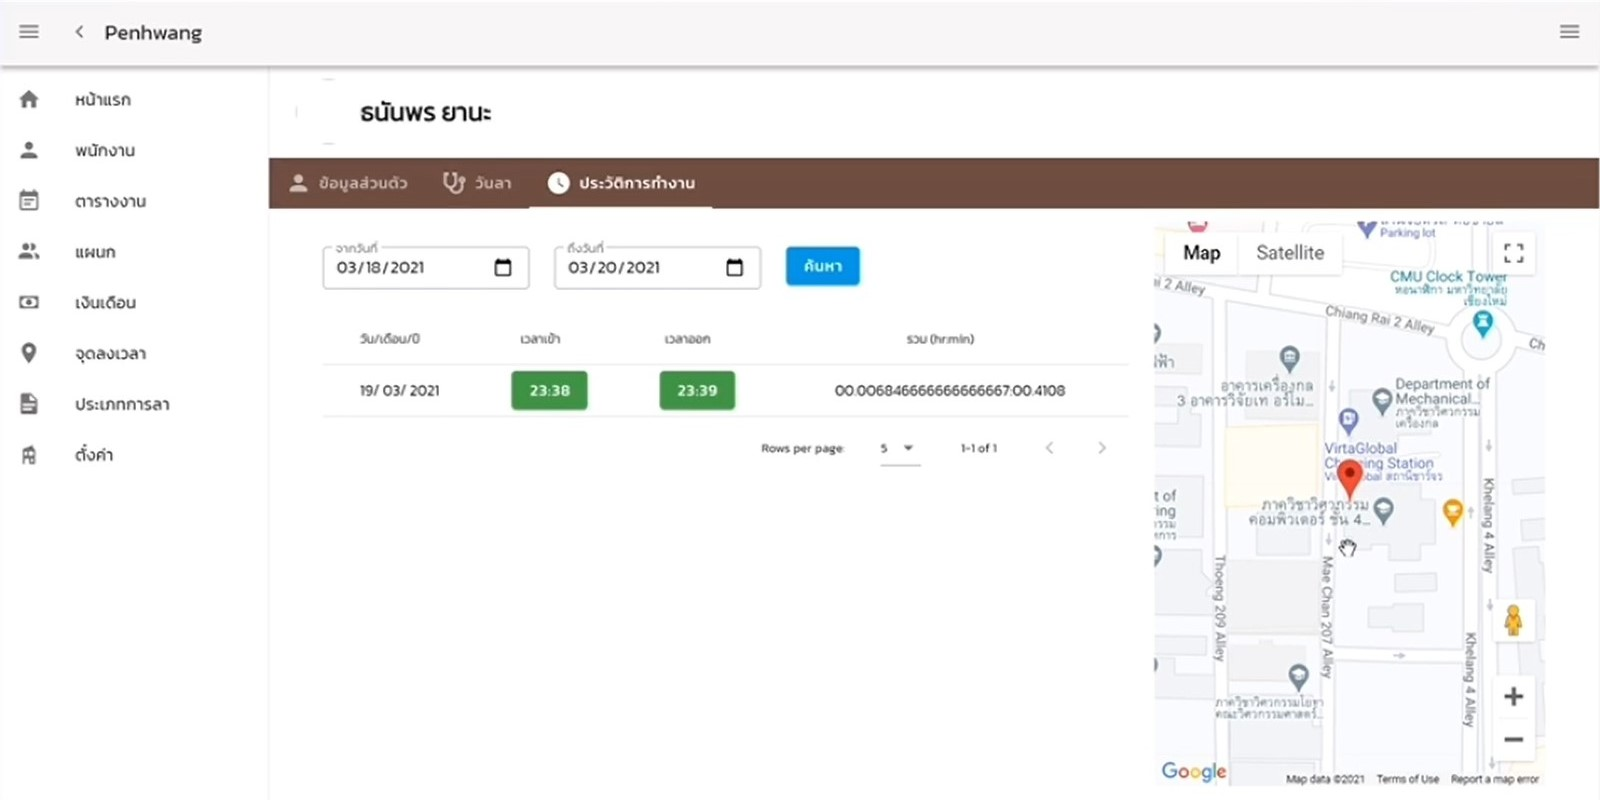
\includegraphics[width=14cm,keepaspectratio]{./images/history.jpg}
  \end{center}
  \caption[รูปแสดงหน้าประวัติการทำงานของพนักงาน]{รูปแสดงหน้าประวัติการทำงานของพนักงาน} 
  \label{fig:history}
\end{figure}

\begin{figure}
  \begin{center}
    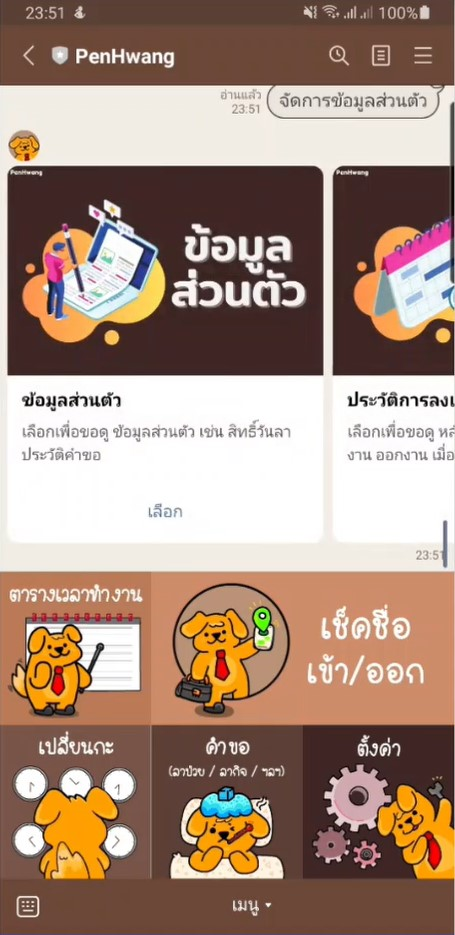
\includegraphics[width=4cm,keepaspectratio]{./images/message_setting.jpg}
  \end{center}
  \caption[รูปแสดงข้อความตอบกลับเมื่อขอตั้งค่า]{รูปแสดงข้อความตอบกลับเมื่อขอตั้งค่า} 
  \label{fig:message_setting}
\end{figure}

\begin{figure}
  \begin{center}
    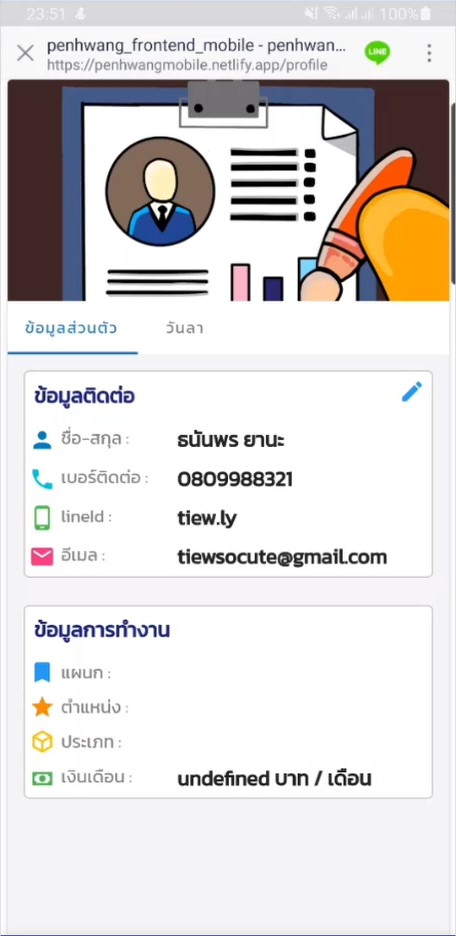
\includegraphics[width=4cm,keepaspectratio]{./images/line_personal_info.jpg}
  \end{center}
  \caption[รูปแสดงหน้าข้อมูลส่วนตัวในโทรศัพท์]{รูปแสดงหน้าข้อมูลส่วนตัวในโทรศัพท์} 
  \label{fig:line_personal_info}
\end{figure} 
 
\begin{figure}
  \begin{center}
    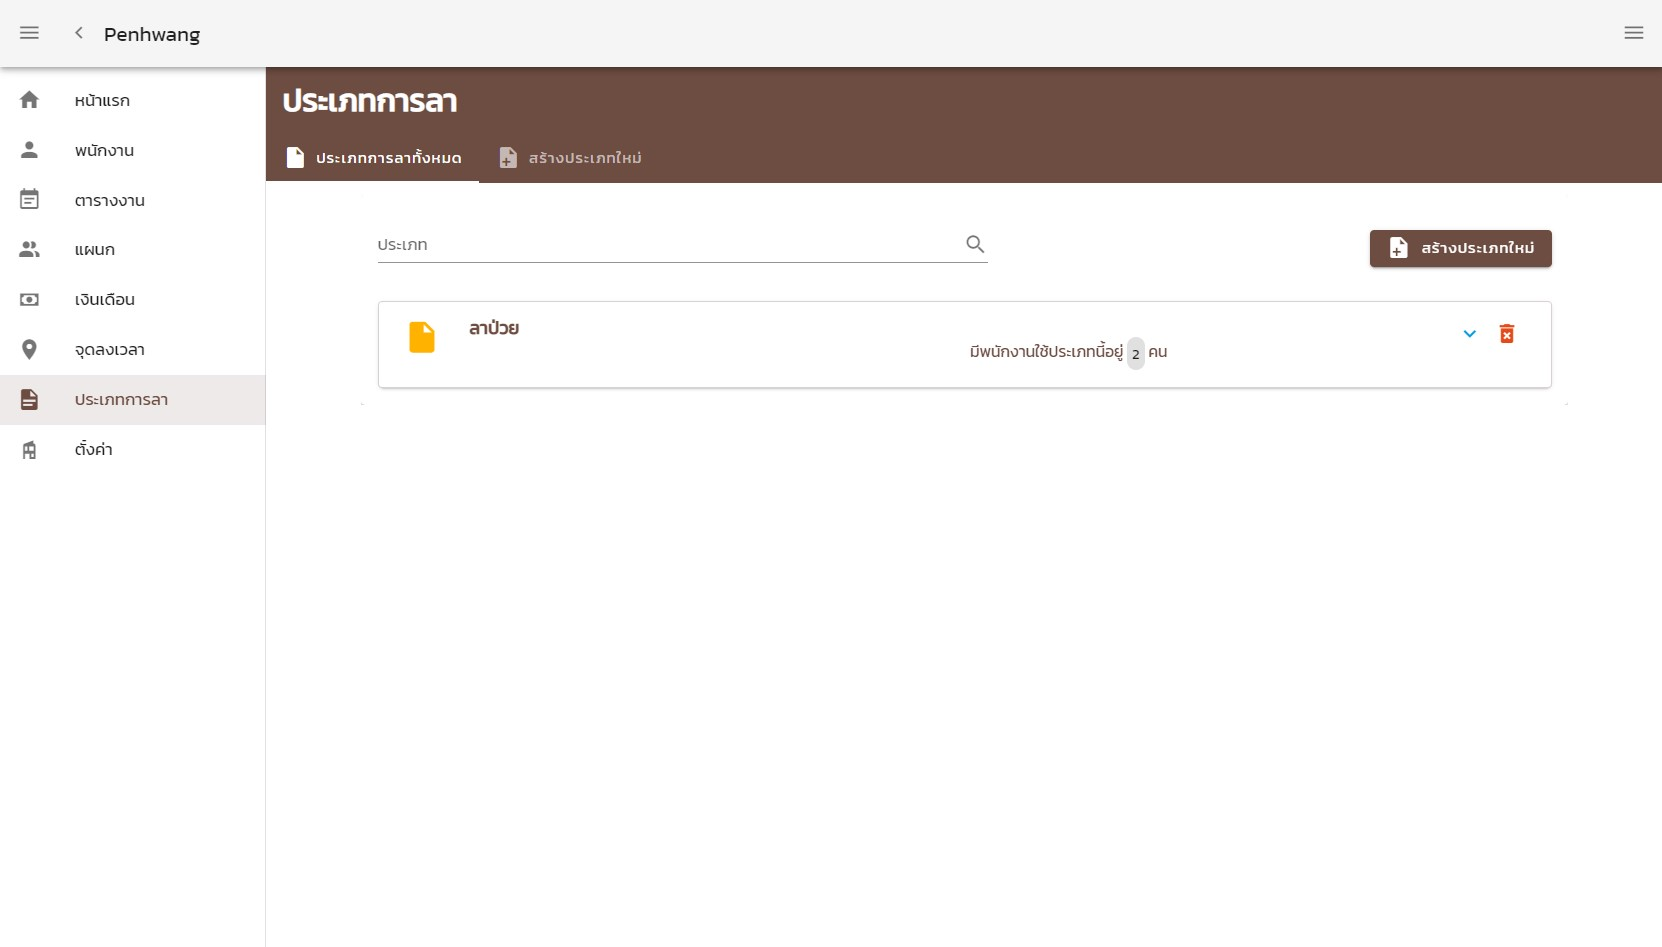
\includegraphics[width=14cm,keepaspectratio]{./images/leave.jpg}
  \end{center}
  \caption[รูปแสดงหน้ารวมของประเภทการลา]{รูปแสดงหน้ารวมของประเภทการลา} 
  \label{fig:leave}
\end{figure}

\begin{figure}
  \begin{center}
    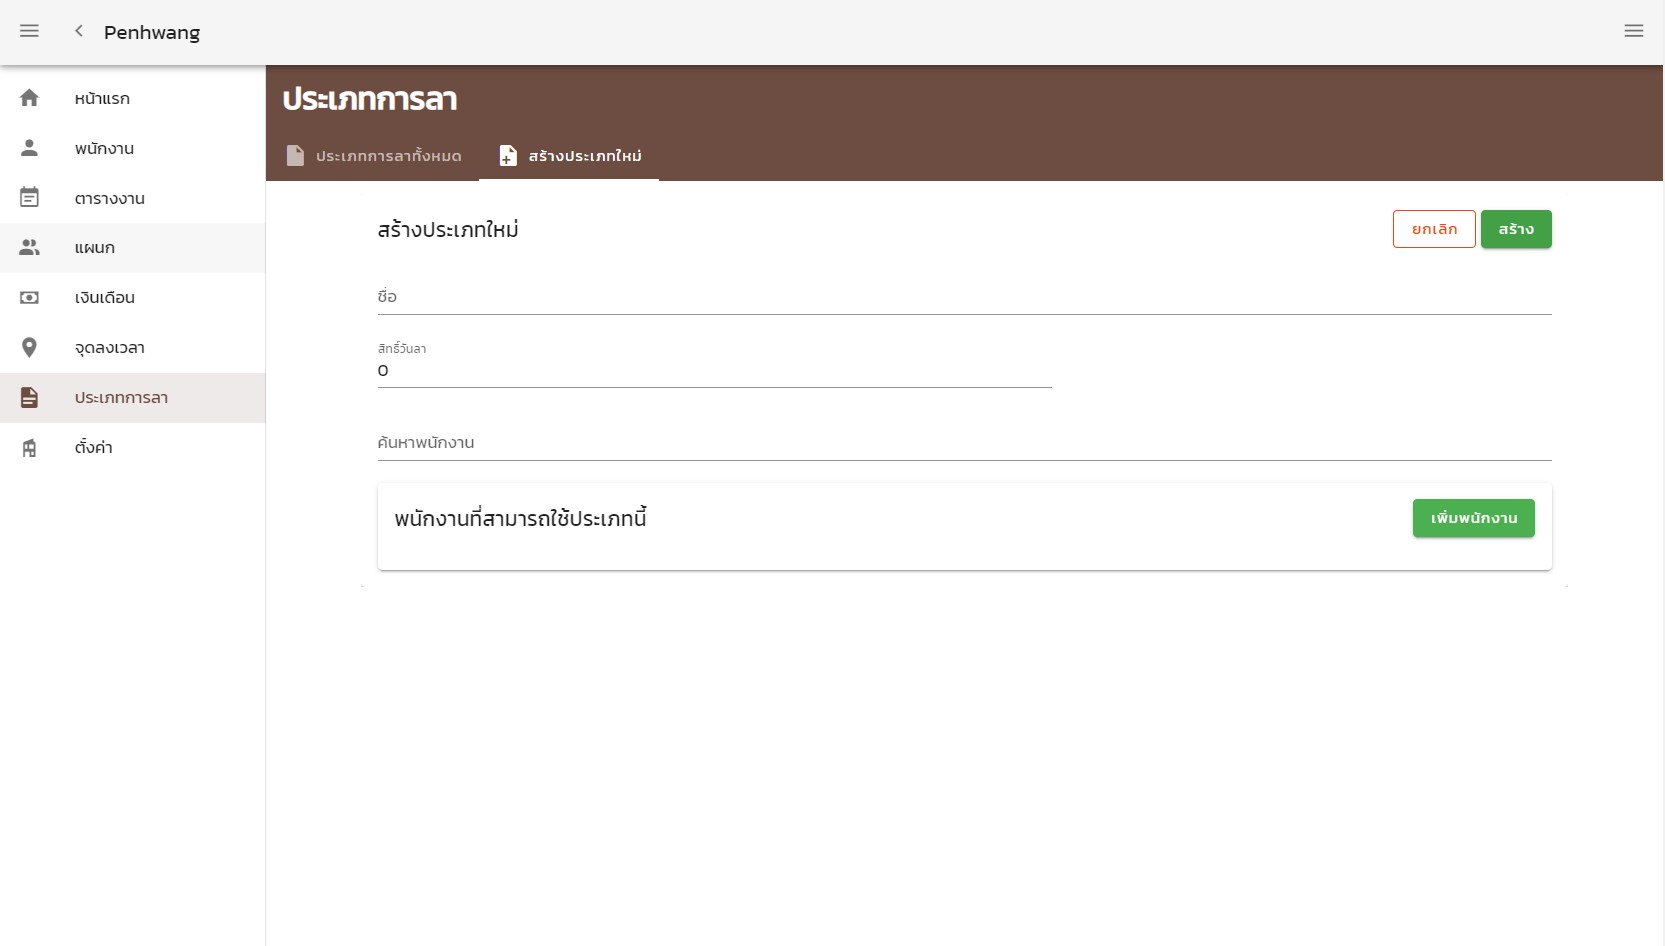
\includegraphics[width=14cm,keepaspectratio]{./images/new_leave.jpg}
  \end{center}
  \caption[รูปแสดงหน้าสร้างประเภทการลาใหม่]{รูปแสดงหน้าสร้างประเภทการลาใหม่} 
  \label{fig:new_leave}
\end{figure} 

\begin{figure}
  \begin{center}
    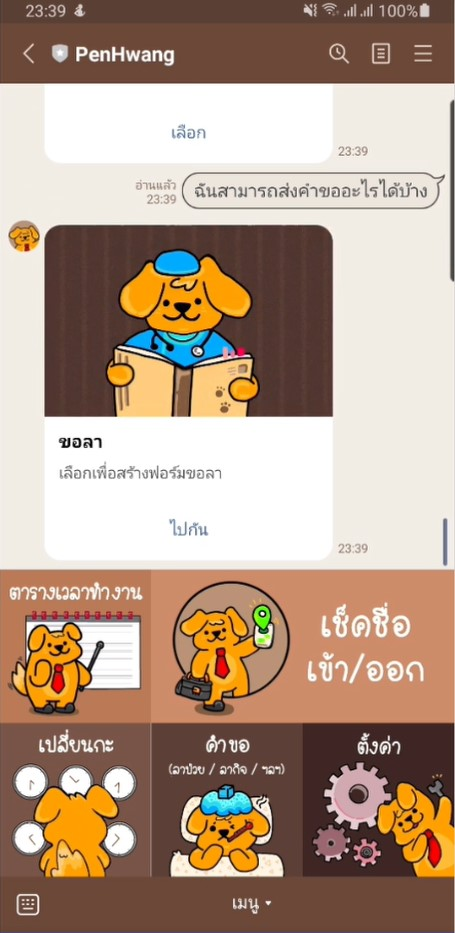
\includegraphics[width=4cm,keepaspectratio]{./images/message_leave.jpg}
  \end{center}
  \caption[รูปแสดงข้อความตอบกลับเมื่อขอลา]{รูปแสดงข้อความตอบกลับเมื่อขอลา} 
  \label{fig:message_leave}
\end{figure}
 
\begin{figure}
  \begin{center}
    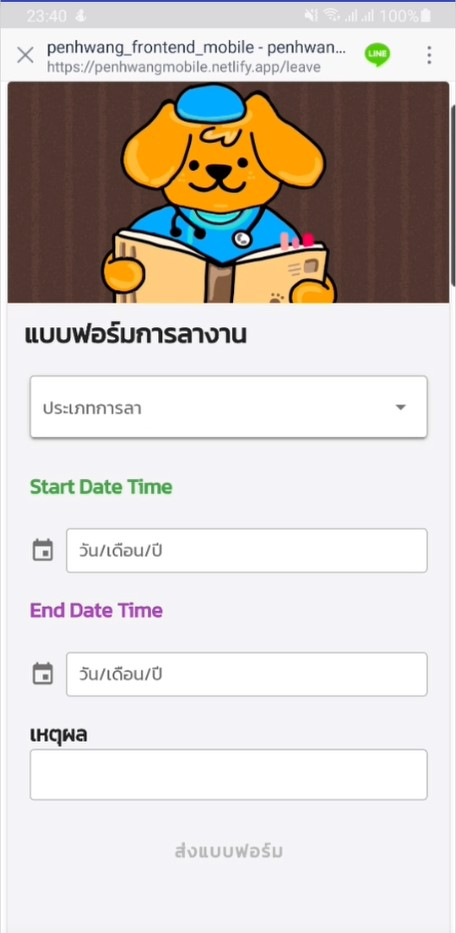
\includegraphics[width=4cm,keepaspectratio]{./images/line_leave.jpg}
  \end{center}
  \caption[รูปแสดงแบบฟอร์มขอลา]{รูปแสดงแบบฟอร์มขอลา} 
  \label{fig:line_leave}
\end{figure}
 
\begin{figure}
  \begin{center}
    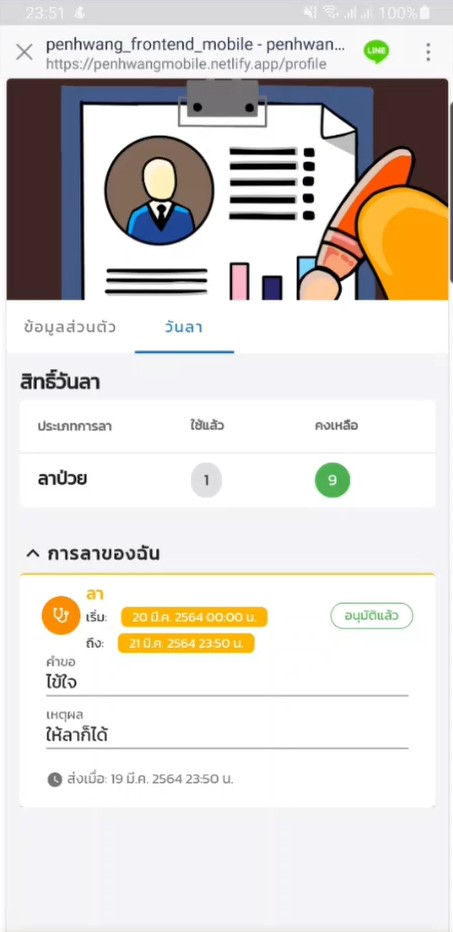
\includegraphics[width=4cm,keepaspectratio]{./images/line_leave_history.jpg}
  \end{center}
  \caption[รูปแสดงประวัติและสิทธิ์การลาในโทรศัพท์มือถือ]{รูปแสดงประวัติและสิทธิ์การลาในโทรศัพท์มือถือ} 
  \label{fig:line_leave_history}
\end{figure}

\begin{figure}
  \begin{center}
    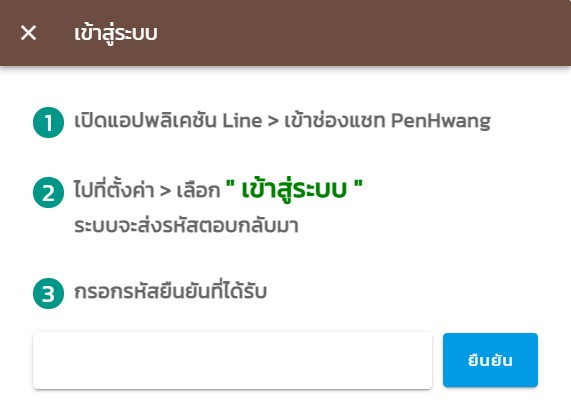
\includegraphics[width=14cm,keepaspectratio]{./images/login.jpg}
  \end{center}
  \caption[รูปแสดงหน้า log-in]{รูปแสดงหน้า log-in} 
  \label{fig:login}
\end{figure}

\begin{figure}
  \begin{center}
    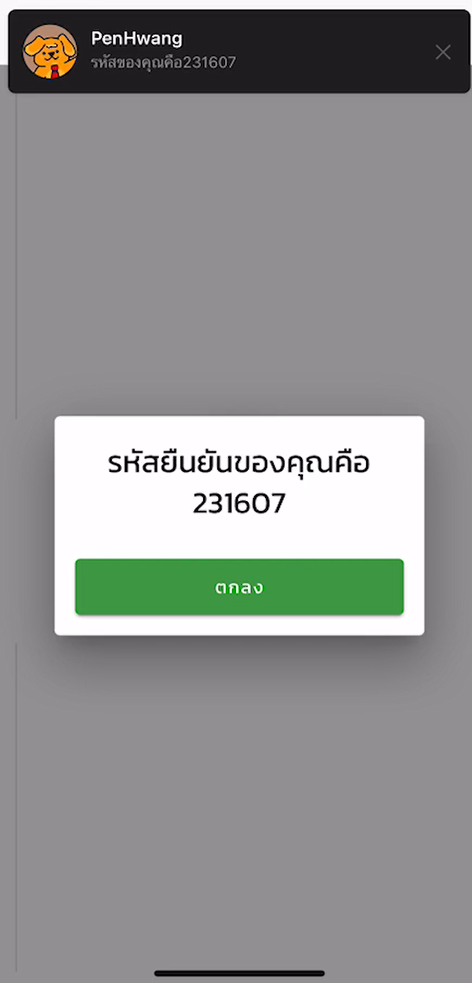
\includegraphics[width=4cm,keepaspectratio]{./images/message_login.png}
  \end{center}
  \caption[รูปแสดงข้อความตอบกลับเมื่อขอ log-in]{รูปแสดงข้อความตอบกลับเมื่อขอ log-in} 
  \label{fig:message_login}
\end{figure}
\ifproject
\chapter{\ifcpe บทสรุปและข้อเสนอแนะ\else Conclusions and Discussion\fi}

\section{\ifcpe สรุปผล\else Conclusions\fi}
\quad “เป็นห่วง” เป็นระบบที่พัฒนาขึ้นเพื่อเป็นทางเลือกในการจัดการเวลาทํางานของพนักงานสําหรับบริษัทที่ต้องการใช้เทคโนโลยีใหม่ ๆ โดยพนักงานสามารถเข้าถึงได้ง่าย ผ่านไลน์แชทบอท 
ดังนั้นจึงไม่ต้องติดตั้งแอปพลิเคชันเพิ่มเติม ระบบออกแบบให้ช่วยลดความผิดพลาดของมนุษย์ จึงง่ายต่อการจัดการ และ ตรวจสอบ ความถูกต้องโดยฝ่ายบุคคล
โดย เป็นห่วง ได้มีการทดสอบการใช้งานเบื้องต้นแล้ว พบว่ามีประโยชน์ต่อผู้ใช้ และ ง่ายต่อการใช้งาน ทั้งนี้ในอนาคตจะต้องมีการทดสอบ 
และสํารวจผลเพื่อตรวจสอบความถูกต้อง และ ความแม่นยําของระบบเพิ่มเติม เนื่องจากสถานการณ์ COVID-19 ในปัจจุบันทําให้ไม่สามารถทดสอบกับผู้ใช้งานทุกบทบาทได้

\section{\ifcpe ปัญหาที่พบและแนวทางการแก้ไข\else Challenges\fi}

% ในการทำโครงงาน เป็นห่วง ไลน์แชทบอทสำหรับจัดการเวลาทำงานของพนักงาน พบว่าเกิดปัญหาหลัก ๆ ดังนี้
% \begin{itemize}
%   \item ข้อมูลมีความสัมพันธ์กันซับซ้อนไม่เหมาะกับการเก็บข้อมูลแบบ NoSQL
%   \item การเชื่อมต่อกันหลายขั้นหลายระบบทำให้การตอบสนองกับผู้ใช้งานช้าลง
%   \item LINE ยังไม่มีรูปแบบที่รองรับสำหรับการทำงานที่ออกแบบไว้ทั้งหมด
%   \item การพัฒนาระบบได้ช้า เนื่องจากไม่ได้ศึกษาเทคโนโลยีที่จะใช้แบบลึกซึ้งก่อนทำงานจริง
% \end{itemize}
ในการทำโครงงาน เป็นห่วง ไลน์แชทบอทสำหรับจัดการเวลาทำงานของพนักงาน พบว่าเกิดปัญหาที่สำคัญประกอบด้วย 
ข้อมูลของพนักงาน บริษัท และ คำขอต่าง ๆ มีความสัมพันธ์กันซับซ้อนไม่เหมาะกับการเก็บข้อมูลแบบ NoSQL 
แต่สาเหตุที่ผู้พัฒนาเลือกใช้ฐานข้อมูลแบบ NoSQL เพราะในช่วงการออกแบบไม่ได้คำนึกถึงการใช้งานทั้งหมด และ firebase 
มีข้อดีคือสามารถ deploy ฐานข้อมูล และ API ที่เขียนขึ้นมาได้ทันที และ ฐานข้อมูลแบบ NoSQL มีความยืดหยุ่นสามารถรองรับความผิดพลาดจากการใส่ข้อมูลได้ 
ปัญหาต่อมาคือ การเชื่อมต่อกันหลายขั้นหลายระบบทำให้การตอบสนองกับผู้ใช้งานช้าลง 
อีกปัญหาคือ แอปพลิเคชัน LINE ยังไม่มีรูปแบบที่รองรับสำหรับการทำงานที่ออกแบบไว้ทั้งหมด 
ปัญหาที่สำคัญสุดท้ายคือ การพัฒนาระบบได้ช้า เนื่องจากไม่ได้ศึกษาเทคโนโลยีที่จะใช้แบบลึกซึ้งก่อนทำงานจริง

\section{\ifcpe%
ข้อเสนอแนะและแนวทางการพัฒนาต่อ
\else%
Suggestions and further improvements
\fi
}

% ข้อเสนอแนะเพื่อพัฒนาโครงงานนี้ต่อไป หรือ สำหรับผู้พัฒนาทีมอื่น ๆ ที่จะทำโครงงานที่คล้ายกันในอนาคต มีดังนี้
% \begin{itemize}
%   \item ในขั้นตอนการออกแบบระบบ ให้คำนึงถึงการนำข้อมูลไปใช้งานด้วย โดยหากการดึงข้อมูลแต่ละครั้งมีความจำเป็นต้องใช้ข้อมูลจากหลายแหล่งพร้อม ๆ กันควรเป็นการเก็บแบบ SQL มากกว่าเพื่อความสะดวกในการจัดการข้อมูล
%   \item หากเลือกที่จะใช้แบบ NoSQL ก็ควรศึกษาประโยชน์ และ ข้อเสีย รวมถึงข้อควรระวังในการออกแบบฐานข้อมูลแบบนี้ด้วย
%   \item นอกจากศึกษาเทคโนโลยีที่จะใช้แล้ว ควรมีการลองนำเทคโนโลยีเหล่านั้นมาใช้งานกับโปรเจคเล็ก ๆ ก่อน เพื่อจะเปลี่ยนแปลง แก้ไขได้ทันที
%   \item หากจะให้ "การใช้งานง่าย" เป็นจุดเด่นของโปรเจค ควรมีการทำ prototype ไปทดสอบกับผู้ใช้งานบ่อย ๆ เพื่อนำข้อคิดเห็นมาปรับปรุง
% \end{itemize}


ข้อเสนอแนะเพื่อพัฒนาโครงงานนี้ต่อไป หรือ สำหรับผู้พัฒนาทีมอื่น ๆ ที่จะทำโครงงานที่คล้ายกันในอนาคต ประกอบด้วย 
ในขั้นตอนการออกแบบระบบ ผู้พัฒนาควรคำนึงถึงการนำข้อมูลไปใช้งานทั้งหมด หมายความว่าต้องออกแบบระบบ และ ฟังก์ชันทั้งหมดก่อนจะเลือกใช้ฐานข้อมูล 
โดยหากการดึงข้อมูลไปใช้งานแต่ละครั้งมีความจำเป็นต้องใช้ข้อมูลจากหลายจุดพร้อม ๆ กันควรเป็นการเก็บแบบ SQL มากกว่าเพื่อความสะดวกในการจัดการข้อมูล 
แต่หากเลือกที่จะใช้แบบ NoSQL ก็ควรศึกษาประโยชน์ และ ข้อเสีย รวมถึงข้อควรระวังในการออกแบบฐานข้อมูลแบบนี้ด้วย 
ต่อไปคือ นอกจากศึกษาเทคโนโลยีที่จะใช้แล้ว ควรมีการลองนำเทคโนโลยีเหล่านั้นมาใช้งานกับโครงงานเล็ก ๆ ก่อน เพื่อให้รู้ผลจากการเพิ่มเทคโนโลยีนี้เข้าไปในระบบ และ เพื่อให้รู้วิธีการใช้งานที่ถูกต้อง 
คำแนะนำข้อสุดท้ายคือ หากผู้พัฒนาต้องการให้ "การใช้งานง่าย" เป็นจุดเด่นของโครงการควรมีการทำ prototype ไปทดสอบกับผู้ใช้งานบ่อย ๆ เพื่อนำข้อคิดเห็นมาปรับปรุง จะส่งผลให้ผลสุดท้ายของโครงการออกมาตรงตามความต้องการของผู้ใช้งานมากกว่าตอนนี้

\fi

\bibliography{sampleReport}

\ifproject
\appendix
\chapter{แผนภาพการออกแบบระบบ}

ในขั้นตอนทำโครงงาน เป็นห่วง เริ่มจากการออกแบบก่อนนำไปสร้างเป็นระบบจริง เนื้อหาในภาคผนวกนี้ประกอบด้วยขั้นตอนการออกแบบการทำงานของฟังก์ชันต่าง ๆ รวมถึงหน้าตาของระบบ ที่เกี่ยวข้องกับโครงงาน 
โดยเนื้อหาจะแบ่งออกเป็นสองส่วนหลัก ๆ คือ 
การออกแบบวิธีการทำงานของระบบซึ่งออกแบบโดยใช้แอปพลิเคชัน Goodnotes และการออกแบบหน้าตาของระบบซึ่งออกแบบโดยใช้โปรแกรม Adobe XD ดังนี้
\begin{figure}
  \begin{center}
    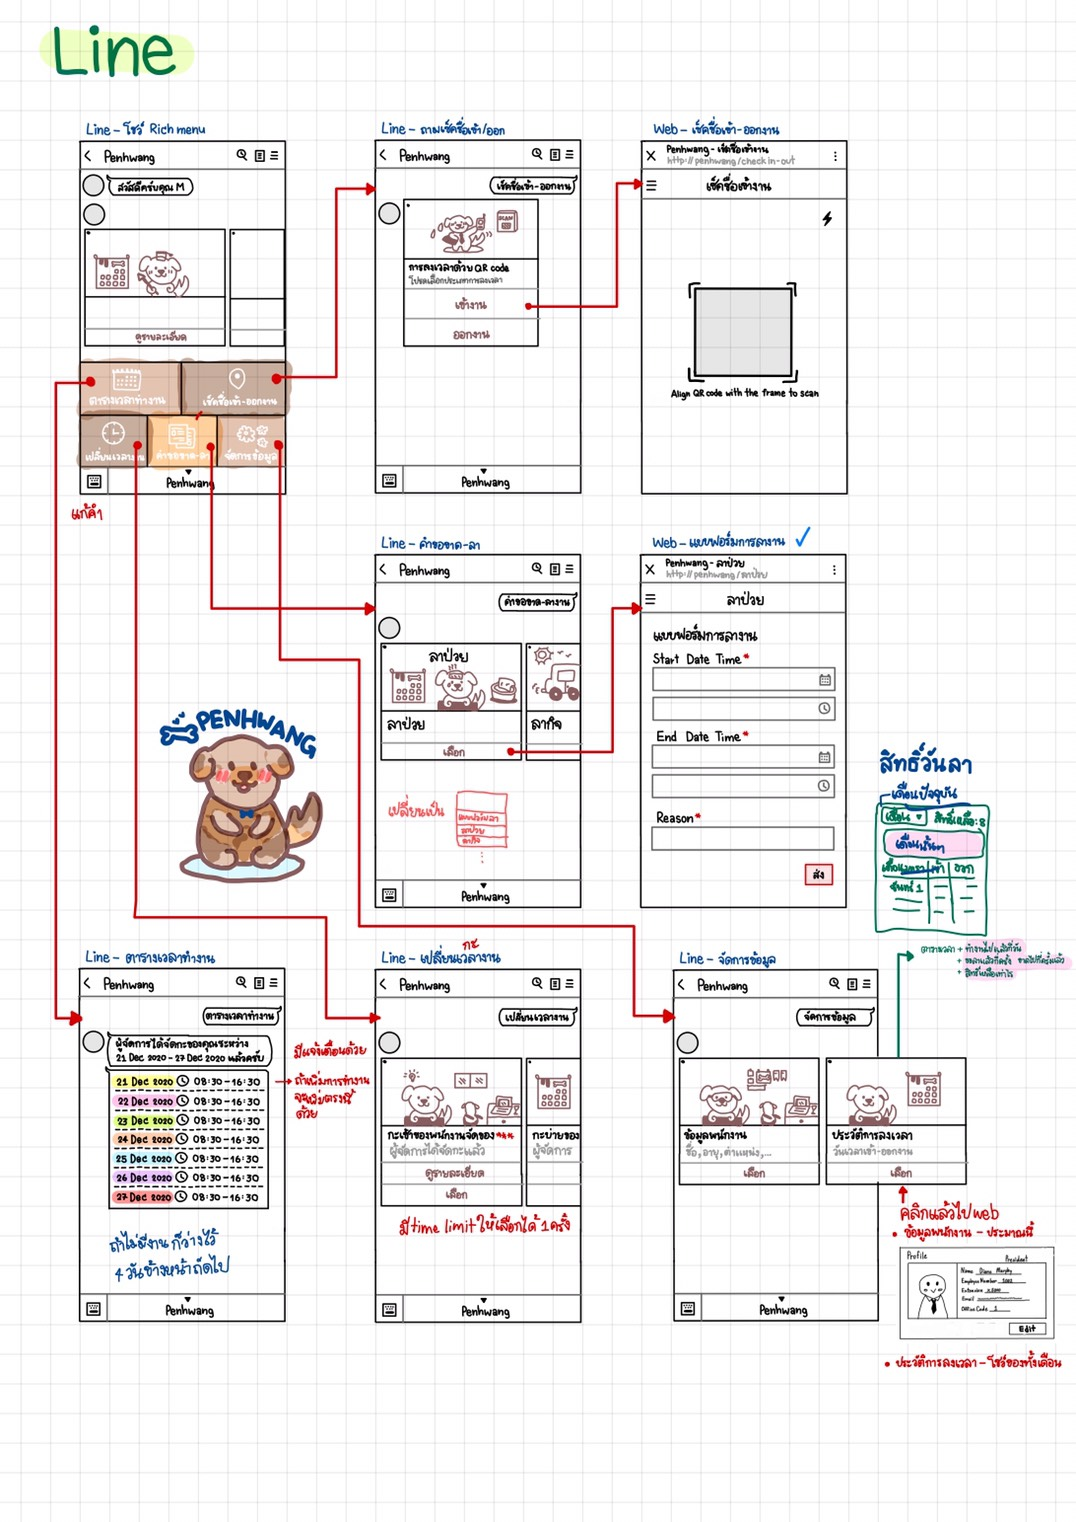
\includegraphics[width=\linewidth]{./images/design1.jpg}
  \end{center}
  \caption[รูปแสดงภาพร่างของ chatbot]{รูปแสดงภาพร่างของ chatbot} 
\end{figure}

\begin{figure}
  \begin{center}
    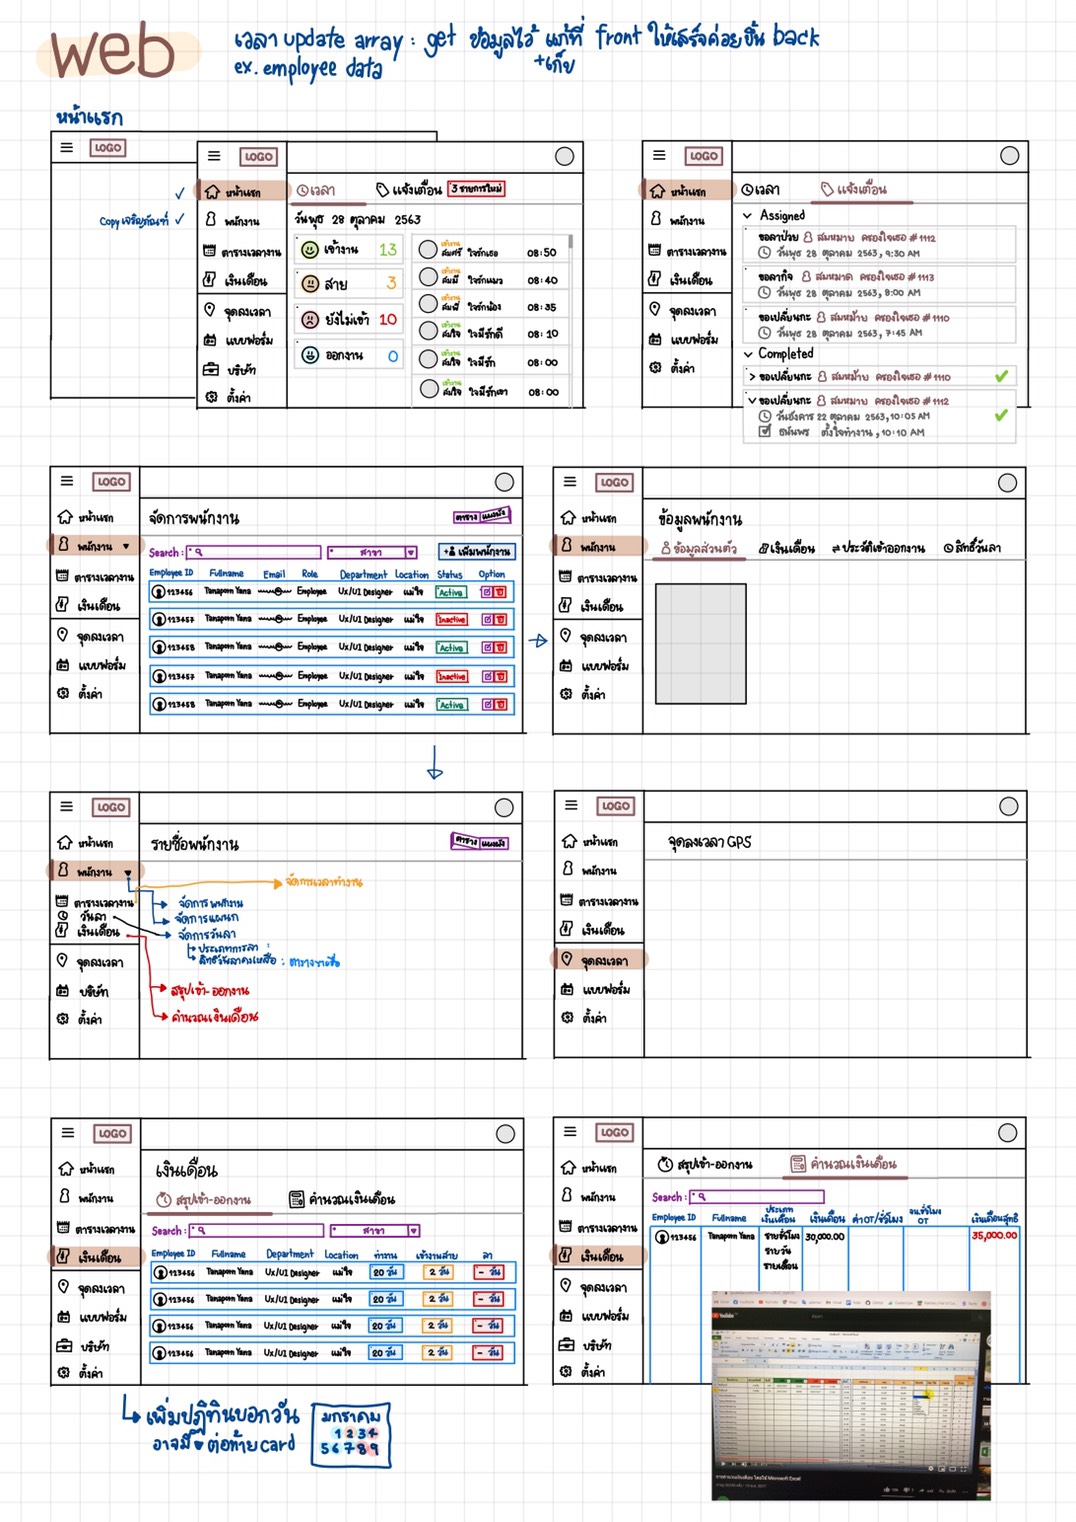
\includegraphics[width=14cm,keepaspectratio]{./images/design3.jpg}
  \end{center}
  \caption[รูปแสดงภาพร่างของเว็บแอปพลิเคชัน]{รูปแสดงภาพร่างของเว็บแอปพลิเคชัน} 
  
\end{figure}

\begin{figure}
  \begin{center}
    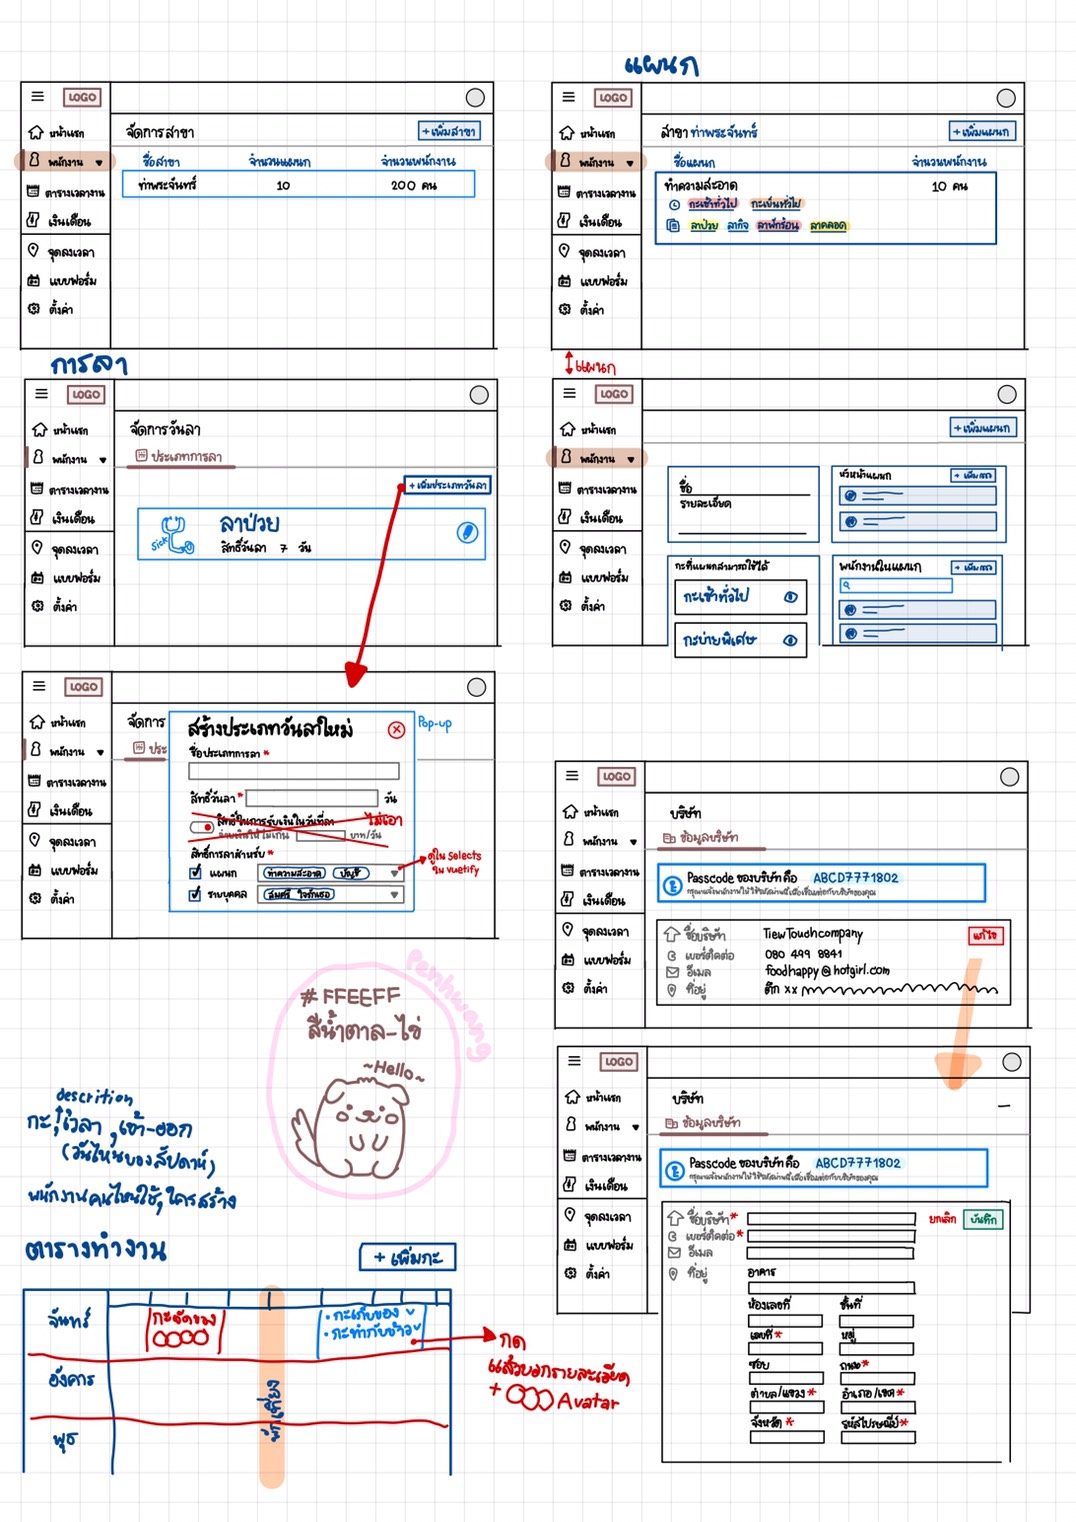
\includegraphics[width=14cm,keepaspectratio]{./images/design4.jpg}
  \end{center}
  \caption[รูปแสดงภาพร่างของเว็บแอปพลิเคชัน2]{รูปแสดงภาพร่างของเว็บแอปพลิเคชัน2} 
  
\end{figure}

\begin{figure}
  \begin{center}
    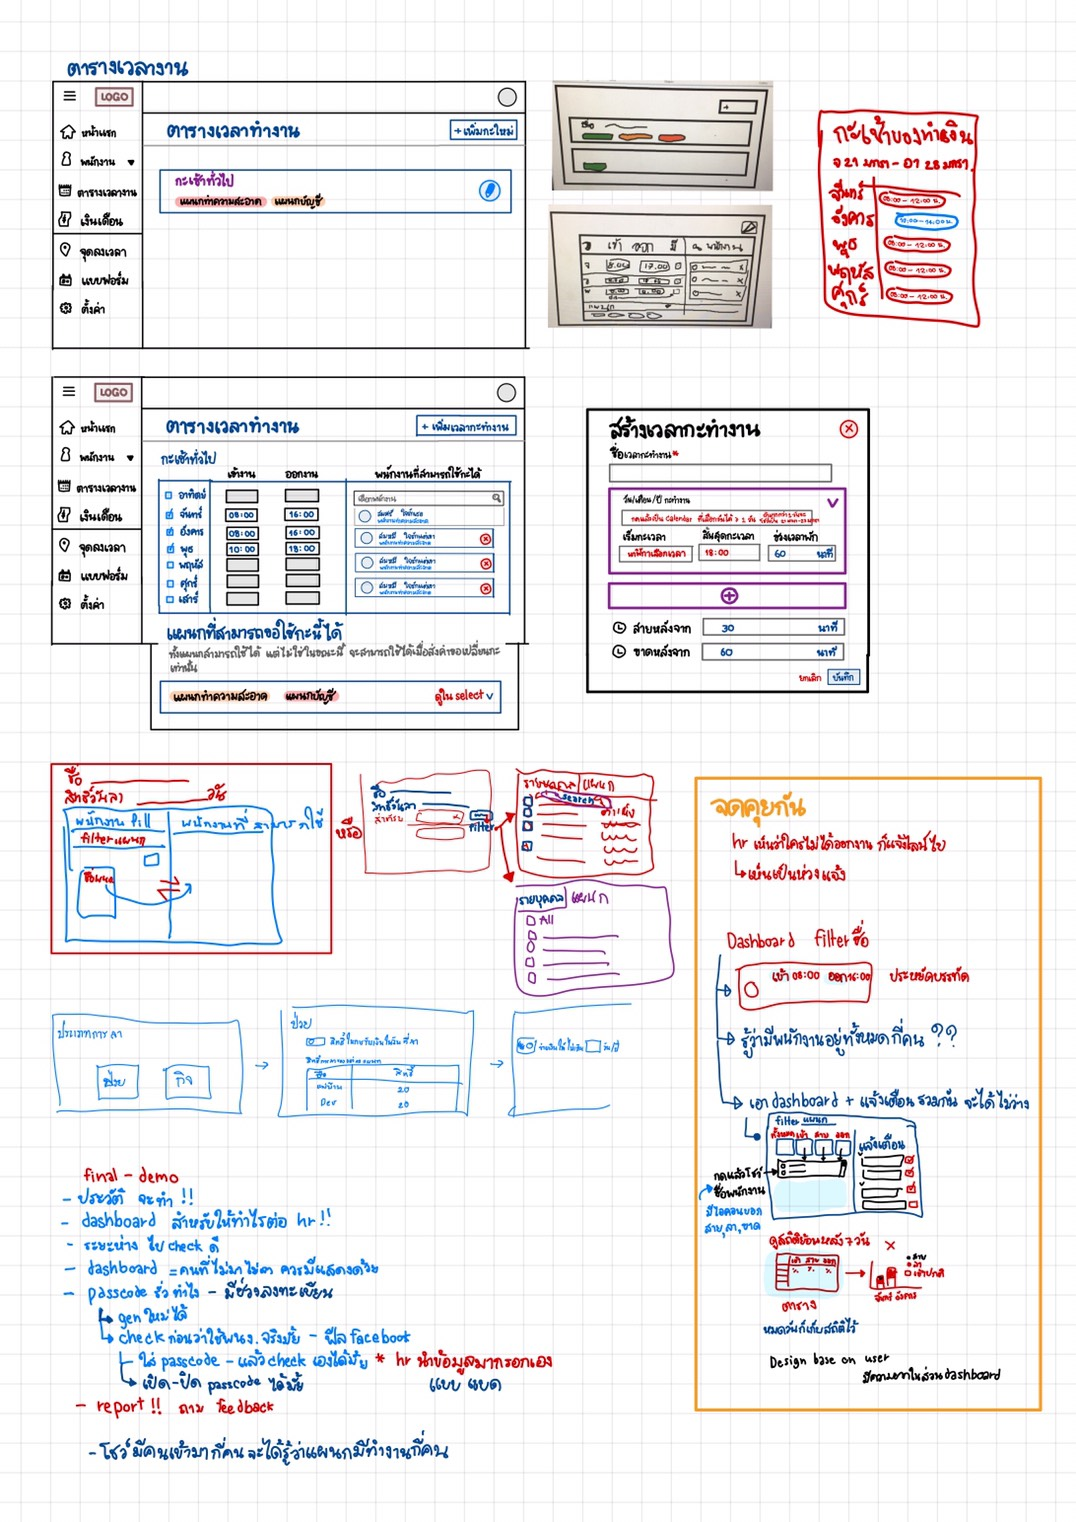
\includegraphics[width=14cm,keepaspectratio]{./images/design5.jpg}
  \end{center}
  \caption[รูปแสดงภาพร่างของเว็บแอปพลิเคชัน3]{รูปแสดงภาพร่างของเว็บแอปพลิเคชัน3} 
  
\end{figure}

\begin{figure}
  \begin{center}
    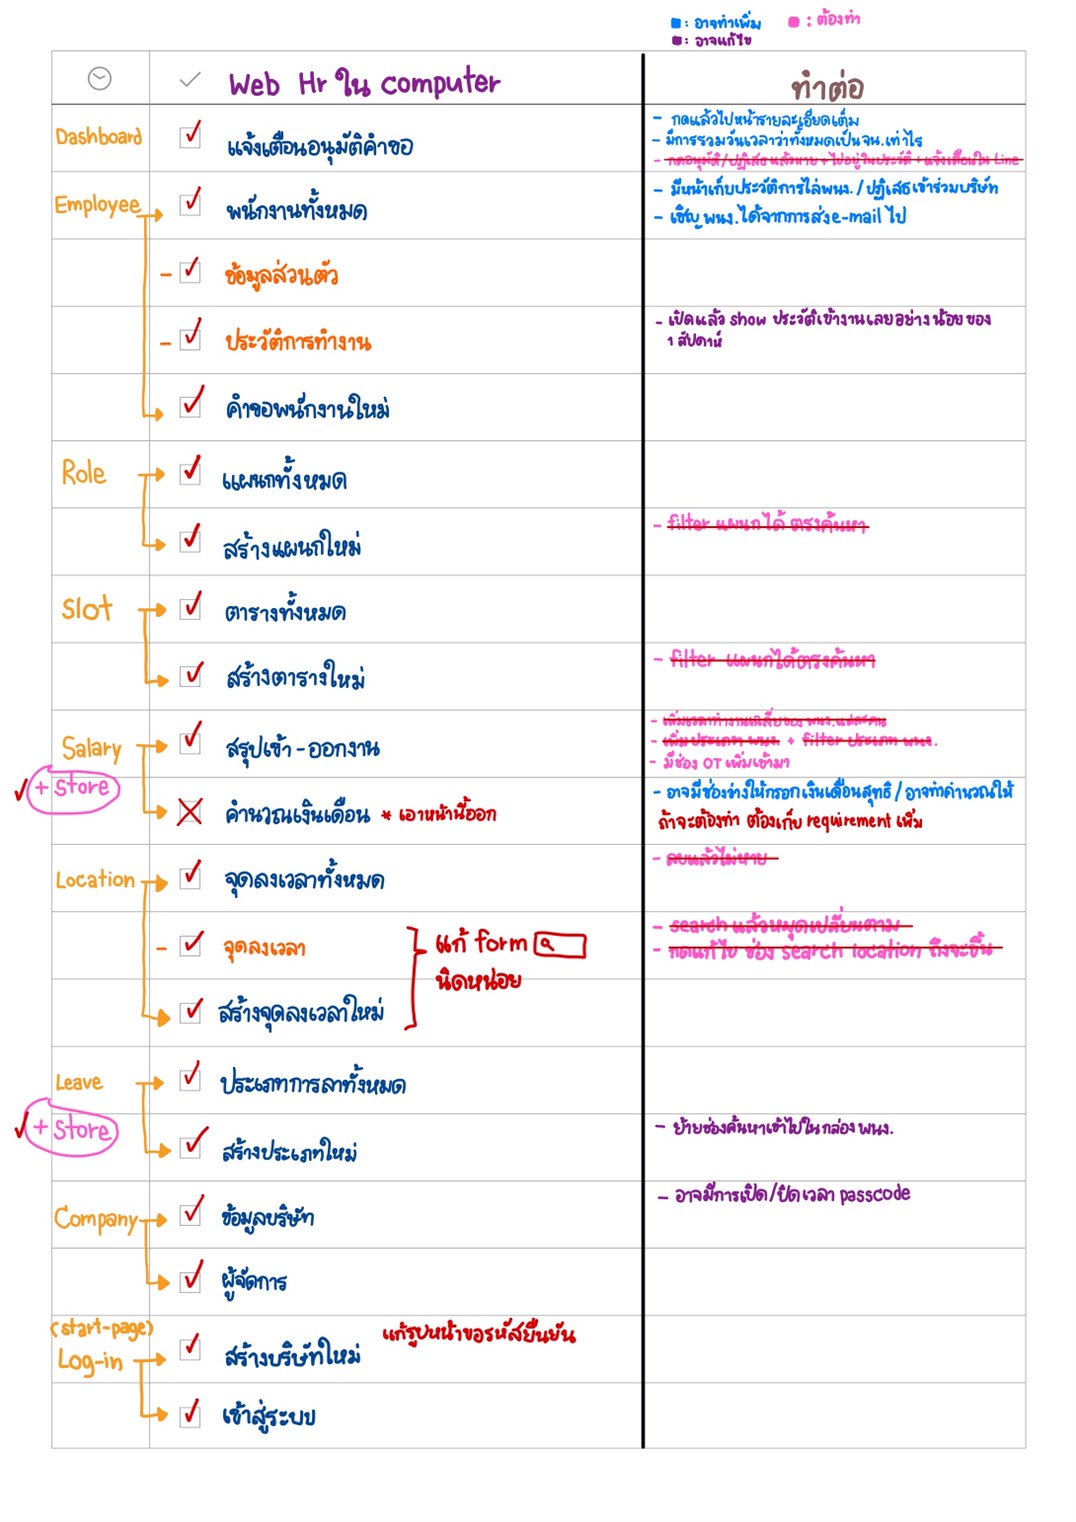
\includegraphics[width=14cm,keepaspectratio]{./images/design7.jpg}
  \end{center}
  \caption[รูปแสดงลำดับขั้นตอนการทำงานและการตรวจสอบความเรียบร้อย]{รูปแสดงลำดับขั้นตอนการทำงานและการตรวจสอบความเรียบร้อย} 
  
\end{figure}

\begin{figure}
  \begin{center}
    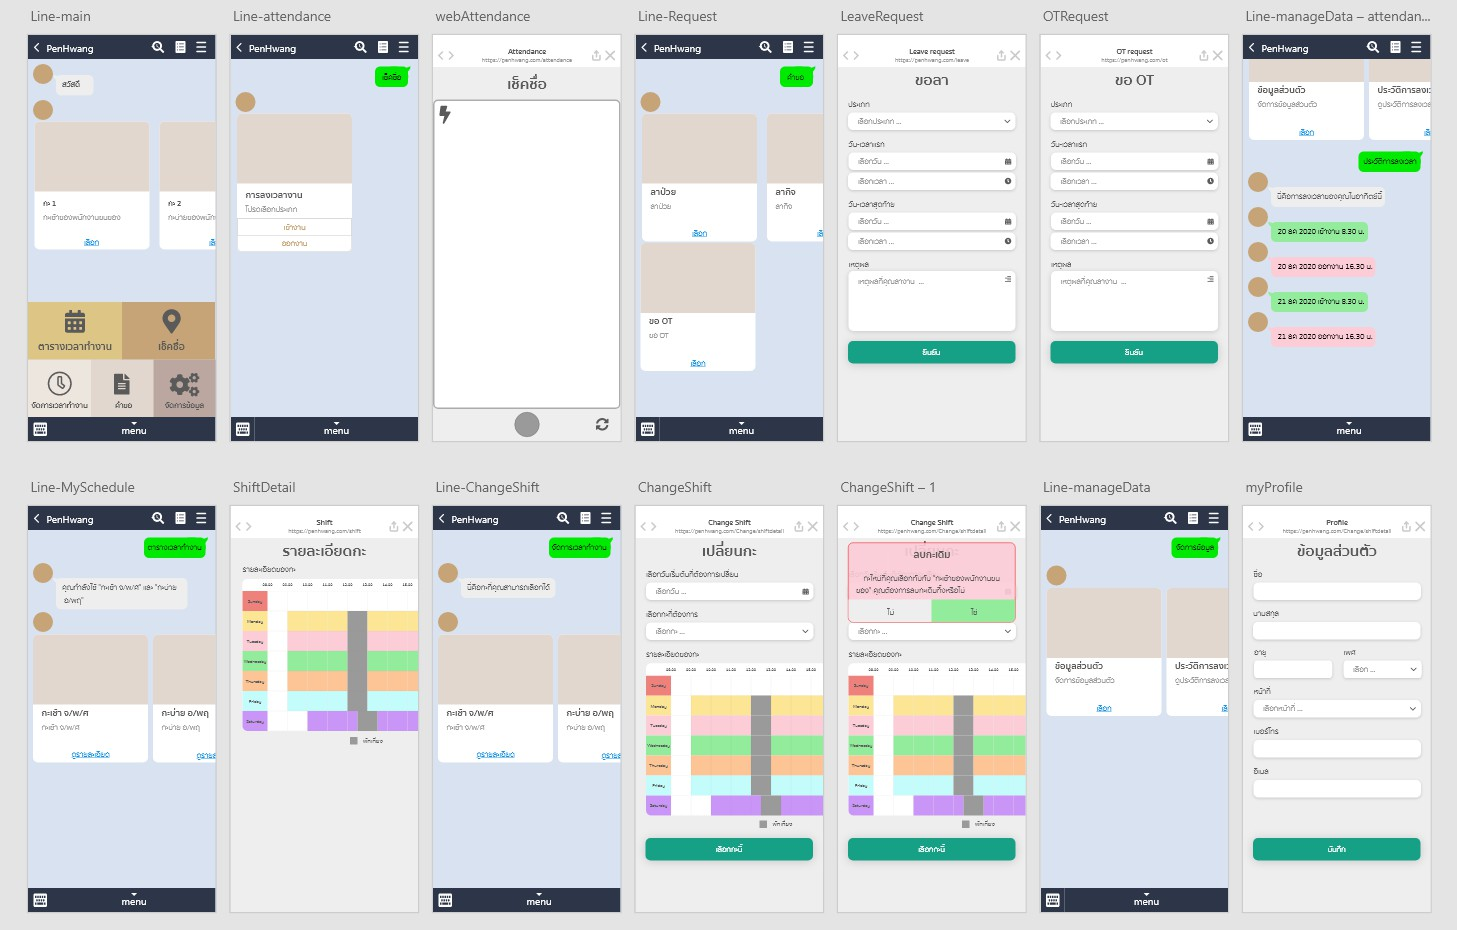
\includegraphics[width=\linewidth]{./images/design_xd.jpg}
  \end{center}
  \caption[รูปแสดงผลจากการออกแบบด้วยโปรแกรม Adobe XD]{รูปแสดงผลจากการออกแบบด้วยโปรแกรม Adobe XD} 
  
\end{figure}

\begin{figure}
  \begin{center}
    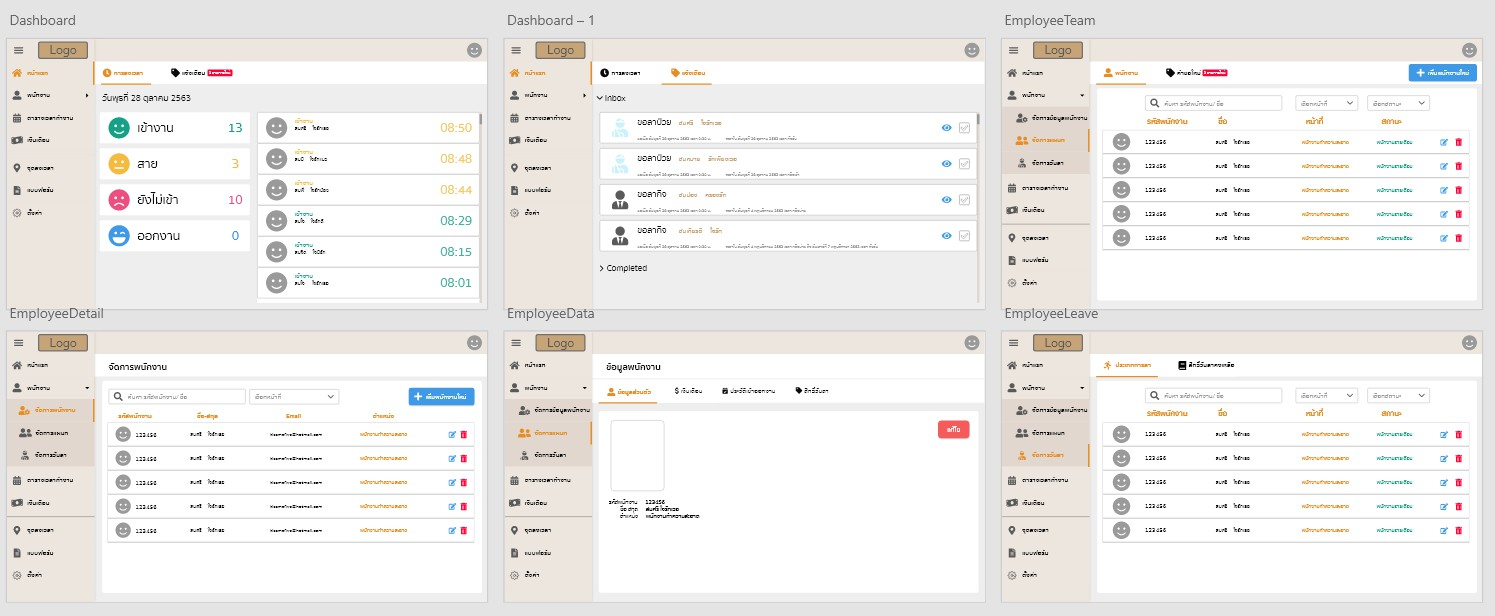
\includegraphics[width=\linewidth]{./images/design_xd2.jpg}
  \end{center}
  \caption[รูปแสดงผลจากการออกแบบด้วยโปรแกรม Adobe XD 2]{รูปแสดงผลจากการออกแบบด้วยโปรแกรม Adobe XD 2} 
  
\end{figure}
% \chapter{\ifcpe คู่มือการใช้งานระบบ\else Manual\fi}
% ฟังก์ชันที่โปรเจคนี้รองรับ และ วิธีการใช้งานมีดังนี้
% \section{สร้างบริษัทของคุณ}



% \section{code จาก GitHub}
% โปรเจคนี้ถูกแบ่งออกเป็น 3 repositories คือ 

% penhwang backend

% \url{https://github.com/TouchySarun/penhwang_backend}, 

% penhwang frontend mobile

% \url{https://github.com/Tiewly/penhwang_frontend_mobile} 

% และ penhwang frontend desktop 

% \url{https://github.com/TouchySarun/penhwang_frontend_desktop} 
% \section{โปรแกรม และ ส่วนเสริมที่จำเป็น}
% \subsection{IDE (Integrated development environment)}
% โดยโปรเจคนี้เลือกใช้ vs code เป็น IDE หาวิธี install ได้จาก \url{https://code.visualstudio.com/}
% \subsection{package manger command}
% โดยโปรเจคนี้เลือกใช้ npm เป็น package manager หาวิธี install ได้จาก npm 

% \url{https://nodejs.org/en/}
% \subsection{ส่วนเสริม}
% หลังจาก install vs code และ npm แล้ว ให้เปิด vs code ขึ้นมาและเปิด terminal โดยใช้คำสั่งลัด "ctrl + shift + p" 
% \begin{itemize}
%   \item nuxt พิมพ์คำสั่ง > npm i -g nuxt
%   \item firebase-npm เปิดไฟล์ penhwang\_backend โดย คลิกที่ File/Open Floder ... แล้วเลือกไฟล์
% จากนั้นเปิด terminal แล้ว install ส่วนเสริม โดยใช้คำสั่ง > npm i -g firebase
%   \item vue2-google-maps เปิดไฟล์ penhwang\_frontend\_desktop โดย คลิกที่ File/Open Floder ... แล้วเลือกไฟล์
% จากนั้นเปิด terminal แล้ว install ส่วนเสริม โดยใช้คำสั่ง 

% > npm i vue2-google-maps
% \end{itemize}
% \subsection{key สำหรับ API ต่าง ๆ}
% ตัวโปรเจคนี้มีความจำเป็นที่จะต้องเชื่อมต่อกับหลาย ๆ API(Application Programming Interface) เช่น firebase และ google map 
% และ แต่ละ API ต้องมี key ในการเชื่อมต่อ โดยต้องนำ key มาจากที่ต่าง ๆ ดังนี้
% \begin{itemize}
%   \item firebase โดยไปที่หน้า firebase console \url{https://console.firebase.google.com/} หากยังไม่มีโปรเจคของตนเองให้ทำการเพิ่มโปรเจคใหม่จากนั้นเข้าไปที่หน้า Project settings/general สิ่งที่ต้องการมีดังนี้
%   \begin{itemize}
%     \item apiKey
%     \item authDomain
%     \item databaseURL
%     \item projectId
%     \item storageBucket
%     \item messagingSenderId
%     \item appendixmeasurementId
%   \end{itemize}
%   นำทุกอย่างที่ต้องการใส่ในไฟล์ db.js
% \end{itemize}
% \begin{itemize}
%   \item firebase โดยไปที่หน้า firebase console \url{https://console.firebase.google.com/} หากยังไม่มีโปรเจคของตนเองให้ทำการเพิ่มโปรเจคใหม่จากนั้นเข้าไปที่หน้า Project settings/general สิ่งที่ต้องการมีดังนี้
%   \begin{itemize}
%     \item apiKey
%     \item authDomain
%     \item databaseURL
%     \item projectId
%     \item storageBucket
%     \item messagingSenderId
%     \item appendixmeasurementId
%   \end{itemize}
%   นำทุกอย่างที่ต้องการใส่ในไฟล์ db.js
% \end{itemize}



%% Display glossary (optional) -- need glossary option.
\ifglossary\glossarypage\fi

%% Display index (optional) -- need idx option.
\ifindex\indexpage\fi

\begin{biosketch}
\begin{center}
  \includegraphics[width=1.5in]{mugshot.jpg}
\end{center}
Your biosketch goes here. Make sure it sits inside
the \texttt{biosketch} environment.
\end{biosketch}
\fi % \ifproject
\end{document}
